\chapter{面向高维金融因子建模的赛马场竞争方法}

\section{问题的提出}
在对冲基金交易决策链条中，第2章已经围绕多资产配置对象识别与资金权重生成问题展开讨论。然而，资产配置结果能否成立，并不只取决于模型是否给出某一组权重，还取决于这些权重背后是否存在稳定、可解释且能够跨市场状态迁移的因子依据。换言之，第3章关注的重点并不是对资产选择作事后说明，而是在高维金融因子空间中识别能够持续支撑资产配置判断的有效信息。

高维金融因子建模因此成为连接资产配置与后续时机判断的重要中间环节。金融市场中的价格与收益并不是由单一线性信号决定的，而是受到交易机制、信息结构和市场参与者行为的共同影响。异质信息交易条件下的买卖价差与成交价格研究说明，价格序列本身已经包含了交易摩擦和信息不对称因素\cite{glosten1985bid}。连续竞价与内幕交易模型进一步表明，市场价格形成过程会受到交易者信息优势和交易冲击的影响\cite{kyle1985continuous}。因此，高维金融因子建模面对的并不只是变量数量过多的问题，还包括不同信息来源在时间维度、资产维度和市场状态维度上的交互关系如何被稳定识别的问题。

在这一背景下，传统降维方法虽然能够在一定程度上压缩变量空间，但在面对高度非线性、强噪声和多源异构的金融因子时，往往难以充分保留因子之间的复杂交互关系。近年来，深度学习和强化学习方法被引入时间序列预测与多因子建模任务，为非线性因子表征提供了新的工具。金融交易中的合成数据增强与深度强化学习研究说明，深度模型可以借助状态扩展和序列决策机制捕捉部分传统线性方法难以表达的动态关系\cite{liu2022synthetic}。不过，高维因子建模的困难并不只在于表达能力不足，还在于模型面对扰动、噪声和分布漂移时能否保持稳健。鲁棒对抗强化学习研究表明，引入对抗扰动有助于检验和提升策略在复杂环境中的稳定性\cite{pinto2017robust}。这也提示本文，第三章不能只依赖单一深度模型的拟合能力，而需要进一步设计能够持续比较、筛选和修正因子表征的动态竞争机制。

从方法论上看，主成分分析的基本作用是将原始变量投影到少数主成分空间，适合概括线性相关结构，但并不能直接完成金融因子的可交易性筛选\cite{abdi2010principal}。因此，本章关注的关键问题是：在高维、强噪声和非平稳环境下，如何通过动态竞争机制持续筛选有效因子表征，并避免模型群体过早收敛到单一、脆弱的因子解释路径。


\subsection{高维金融因子的非对称竞争关系}
在第2章完成投资组合管理任务并形成多资产配置入口之后，本章进一步将研究对象转向资产配置背后的因子依据层面。对于多资产交易任务而言，组合权重并不是孤立生成的结果，而是建立在一组能够解释收益来源、风险暴露和市场状态变化的候选因子之上。因此，本节关注的不是简单增加因子数量，也不是仅对原始变量进行压缩，而是讨论高维金融因子在不同市场环境下为何会呈现强弱差异、替代关系和阶段性失效。换言之，高维金融因子并不是同质变量集合，不同因子对收益预测、风险识别和资产选择的贡献存在明显差异，这构成了后续赛马场竞争机制需要处理的基本问题。

从方法层面看，传统降维方法能够压缩变量空间，但其主要目标通常是保留总体结构、局部邻近关系或方差贡献，并不直接等同于筛选具有交易含义的金融因子。相关降维评估研究表明，高维数据在降维过程中容易出现结构信息损失和局部关系扭曲的问题\cite{espadoto2019toward}。这一问题在金融因子场景中会被进一步放大，因为部分因子虽然总体方差贡献并不突出，却可能在特定市场状态、极端行情或风险切换阶段具有较强解释价值。因而，如果只依赖静态降维结果判断因子重要性，可能会将短期波动较弱但交易含义明确的变量提前压缩掉。

静态深度表示模型在一定程度上缓解了线性降维的表达能力不足问题。表示学习研究说明，深度模型可以通过多层非线性变换学习复杂数据表征\cite{bengio2013representation}。但是，在金融市场中，表征能力增强并不必然意味着因子解释路径稳定。模型可能在训练样本中捕捉到局部有效的非线性组合，却难以保证该组合在样本外、跨周期或不同资产类别之间持续有效。因此，本章所讨论的高维因子建模，不只是寻找更复杂的表示函数，而是需要判断不同候选因子在动态市场环境中是否仍具备稳定的解释力和可迁移性。

进一步看，不同金融因子之间并非始终保持平等、独立和静态的关系。某些因子在趋势行情中具有较强预测能力，却可能在震荡行情中失效；某些因子单独使用时贡献有限，但与波动率、流动性或基本面变量组合后能够增强风险识别能力；还有一些因子在样本内表现突出，却可能只是由特定时期的偶然相关驱动。演化博弈相关研究为理解主体之间的动态竞争和策略调整提供了可借鉴视角\cite{chang2025survey}。借助这一视角可以看到，高维因子空间中的有效信息并不是一次性固定下来的，而是在不同市场状态下持续发生相对强弱变化。所谓非对称竞争，正是指不同因子在信息含量、稳定性、可解释性和适用场景上并不均衡，其竞争结果会随市场环境变化而调整。

从金融含义上看，因子不是普通统计变量，而是与风险补偿和收益来源相联系的结构化特征。经典多因子模型将股票与债券收益分解为共同风险因子，为高维因子建模提供了资产定价层面的基础参照\cite{fama1993common}。这说明，因子筛选不能只看统计拟合效果，还要说明该因子是否对应可解释的风险暴露或收益来源。五因子模型进一步把盈利能力、投资等维度纳入收益解释框架，表明有效因子往往同时具有统计有效性和经济含义\cite{fama2014five}。因此，在本章语境下，因子竞争并不是单纯比较预测误差大小，而是比较不同因子表征能否持续支撑资产配置判断、风险解释和后续时序结构识别。

随着候选因子数量不断扩展，“因子动物园”问题会进一步放大冗余特征、偶然相关和多重检验风险。因此，因子筛选不能只依赖样本内拟合表现，还需要关注其跨周期稳定性与经济解释能力\cite{feng2020taming}。这一点对本章尤为重要：如果模型只在大量候选因子中寻找短期最优组合，就可能把偶然有效的弱相关变量误判为稳定因子；如果模型只保留传统意义上的主导变量，又可能忽略在局部行情中具有边际贡献的长尾因子。因而，高维因子建模需要在“防止冗余因子干扰”和“保留潜在有效弱信号”之间取得平衡。

金融市场的非平稳性进一步加剧了这种平衡的难度。资产收益及其特征结构会随着宏观环境、交易制度、市场情绪和风险补偿机制的变化而不断调整。资产定价中的因子学习研究说明，因子暴露和收益解释关系并不是固定不变的\cite{KELLY2019501}。对本章而言，这一结论强调的是因子有效性本身具有状态依赖性：同一因子在不同市场阶段可能对应不同的收益解释和风险补偿含义。相关研究也提示，金融预测中的有效特征会受到样本区间和市场状态变化的影响\cite{repec:fau:wpaper:wp2024_26}。由此可见，因子层面的暴露变化与特征层面的有效性变化会共同影响模型对候选因子的筛选判断。这意味着，在某一阶段表现较强的因子，可能在市场状态转换后迅速退化；而在常规区间中不显著的因子，也可能在极端行情或结构切换阶段提供额外信息。

在这种背景下，依赖固定表示结构的静态模型一旦遭遇分布漂移，容易出现样本外泛化能力下降的问题。分布变化与泛化研究说明，当训练分布和测试分布之间存在偏移时，模型需要关注跨环境稳定性，而不能只依赖单一样本分布下的拟合结果\cite{scholkopf2021toward}。对应到金融因子建模中，这意味着模型不仅要识别当前样本中最强的因子组合，还要避免过早排除在未来状态中可能重新发挥作用的候选因子。高维估计误差也会进一步传导到后续组合权重与风险暴露之中。协方差收缩研究表明，在样本有限且变量维度较高时，直接使用样本协方差矩阵容易导致估计不稳定\cite{ledoit2004honey}。这一问题首先体现为风险结构估计的不稳定：因子之间的协方差关系一旦被噪声放大，后续组合权重就可能对局部样本特征过度敏感。参数估计误差所引发的组合优化困境也说明，样本内最优并不必然对应样本外稳健\cite{michaud1989markowitz}。因此，高维因子建模不仅要关注因子本身的预测能力，还要关注其估计误差是否会在组合优化环节被进一步放大。

因此，高维金融因子建模的关键困难，并不只是对静态样本进行拟合，而是如何在分布持续变化的环境中识别仍具有解释力和预测价值的因子结构。深度学习与强化学习在金融交易中的应用表明，序列模型和状态扩展机制能够帮助模型捕捉部分传统线性方法难以表达的动态关系\cite{liu2022synthetic}。但是，单一模型即使具备较强非线性表达能力，也难以保证其因子表征始终稳健。基于上述分析，本章引入赛马场竞争机制，并将其定位为一种面向高维因子空间的动态筛选逻辑：通过模型群体之间的持续比较、更新和知识迁移，识别在不同市场状态下相对稳定且具有解释意义的因子表征。与第2章侧重投资组合管理和资产配置不同，本章重点说明资产选择背后的因子依据如何形成，并为后续时序结构识别提供更可靠的输入基础。

\subsection{传统因子建模中的过早收敛困境}
上一节从因子层面说明了高维金融因子并非同质变量集合，不同因子在收益解释、风险暴露和市场状态切换中的作用存在非对称差异。进一步看，即使模型具备较强的非线性表达能力，训练过程本身也可能放大这种非对称性：早期被模型捕捉到的强信号会在后续迭代中被持续强化，而弱幅度但具有解释价值的长尾因子、阶段性因子和跨周期因子则可能被过早压缩或排除。由此形成的过早收敛，并不是简单的训练轮次不足问题，而是模型在高维因子空间中提前固化到局部有效解释路径的问题。

传统依赖线性假设的特征工程方法，在刻画高维金融变量之间的非线性依赖关系及复杂联合分布时存在明显局限。深度生成模型为高维表征学习提供了新的工具，其中变分自编码器通过潜变量建模与变分推断，能够从高维数据中学习连续且具有结构性的隐表示\cite{kingma2014autoencoding}。这种潜变量思想说明，高维因子可以被压缩到更紧凑的表示空间中，但潜变量压缩解决的是表示组织问题，并不直接等同于有效因子的持续筛选；压缩后的表示是否保留稳定的金融解释，仍需要结合收益预测、风险暴露和跨周期表现进一步判断。随机反向传播与近似推断方法为深度生成模型中的潜变量学习提供了可训练路径\cite{rezende2014stochastic}。这种可训练性使模型能够在高维因子空间中形成潜在表示，但训练目标仍主要围绕重构质量和潜在分布约束展开。其目标函数通常由重构项与基于库尔贝克—莱布勒散度的正则项共同构成\cite{kullback1951information}。这类正则约束有助于稳定潜在空间，但在金融场景中，平滑的潜在分布并不必然意味着弱信号、长尾信号和跨周期信号能够被持续保留。与以重构和潜在空间正则为主的模型不同，生成对抗网络进一步把分布学习放入生成器与判别器之间的博弈过程中，在非线性分布拟合与样本生成方面展现出较强能力\cite{goodfellow2014generative}。不过，对抗学习强调分布匹配，仍需进一步回答模型是否会在训练早期过度强化少数短期占优的因子表征，以及这类表征能否在市场状态变化后得到及时校正。

在更具体的金融时序预测任务中，堆叠自编码器与长短期记忆网络相结合的研究说明，深度表示学习可以从复杂价格序列中提取非线性特征，并为后续预测任务提供更丰富的状态表达\cite{ding2020deep}。这类方法表明，非线性表征能够改善部分金融预测任务，但其重点仍主要落在单个模型在固定训练流程中的表达能力上。对于本章而言，更关键的问题并不是模型能否拟合复杂序列，而是当候选因子数量较多、市场状态不断切换时，模型群体能否持续比较不同因子路径的有效性，并避免所有模型同时收敛到同一类短期强信号。

金融时间序列通常表现出尖峰厚尾、波动聚集和分布偏移等特征，这使得生成模型的训练稳定性本身也成为重要问题。相关研究从目标函数和距离度量角度改进生成对抗训练，为缓解分布学习过程中的不稳定性提供了思路\cite{arjovsky2017towards}。这一类方法说明，改变分布度量可以改善训练过程，但它主要解决的是对抗学习能否稳定推进的问题，而不是高维因子是否被持续筛选的问题。梯度惩罚机制被用于增强Lipschitz约束，从而改善对抗训练的稳定性与鲁棒性\cite{gulrajani2017improved}。这提示本文，训练稳定性是必要条件，但如果模型结构和更新规则缺少差异化竞争，稳定训练也可能只是稳定地强化既有优势路径。扩散模型通过逐步去噪过程学习数据分布，为复杂分布建模提供了新的思路\cite{ho2020denoising}。然而，复杂分布建模能力的提升仍不等于动态因子筛选机制的形成，尤其不能自动保证弱信号、长尾信号和跨周期信号在训练过程中被保留。

从潜在表示与金融定价结合的角度看，对抗自编码器将重构学习与对抗训练结合起来，使潜在表示在重构观测数据的同时更接近预设先验分布\cite{makhzani2015adversarial}。这类方法对于高噪声数据的潜在表示学习具有启发意义，但其核心仍是使潜在空间更加规整，而不是直接刻画因子之间的动态竞争关系。联合编码与生成的对抗表示学习方法进一步增强了潜变量与观测数据之间的协调性\cite{donahue2017adversarial}。这种协调性对于金融数据建模具有参考价值，但在非平稳市场中，观测数据与潜变量之间的对应关系会随市场状态变化而改变，因而仍需要后续机制持续检验表征是否过早固化。

在资产定价场景中，带工具变量的主成分分析尝试从资产特征中学习条件风险暴露，为高维因子提取提供了更贴近金融问题的统计框架\cite{kelly2020instrumented}。自编码器资产定价模型也说明，非线性表示学习可以用于从大量资产特征中提取潜在定价结构\cite{gu2021autoencoder}。这两类研究表明，深度表示并非脱离金融含义的纯技术工具，而可以服务于风险暴露和资产定价结构的识别。进一步看，面向数字金融网络经验资产定价的多空双模式知识蒸馏框架说明，模型间知识传递不仅可用于压缩模型，也可服务于多空结构下的因子表征迁移\cite{yi2024longshort}。但是，知识迁移本身也存在方向性风险：若成熟模型已经过度依赖旧市场状态下的优势因子，直接传递其表征可能会把既有偏差延续到新模型之中；若新生模型的差异化探索缺少反向约束，又可能引入噪声因子并破坏已有稳定表征。因此，知识传递必须与动态竞争、筛选和校正机制结合，才能真正缓解过早收敛。

然而，金融时间序列具有较强的非平稳性与分布漂移特征，训练阶段学习到的分布结构往往难以直接推广到新的市场环境中。分布鲁棒优化研究从不利分布扰动下的泛化角度说明，模型训练不能只依赖单一经验分布下的拟合表现\cite{sagawa2020distributionally}。针对时间序列生成任务，时间序列生成对抗网络将对抗学习与时间监督机制结合，用于保留序列的动态依赖结构\cite{yoon2019time}。这些研究共同提示，金融时序建模既需要复杂表征能力，也需要对分布变化和动态依赖保持敏感。基于这一背景，本章关注的不是单个模型拟合能力的继续堆高，而是在高维因子空间中建立“非对称竞争—过早收敛识别—动态选优修正”的训练闭环，使有效因子能够在模型群体的持续竞争中被筛选、保留和更新。


\section{相关工作}
围绕高维金融因子建模，已有研究主要集中在统计降维、深度表示学习与多模型集成三个方向。统计降维方法侧重压缩变量空间，深度表示学习方法强调非线性特征提取，多模型集成方法则利用模型差异性改善预测稳定性。这些研究构成了金融因子建模的重要基础，但在非平稳市场环境下，仍然容易出现因子表征固化、有效因子与噪声因子难以持续区分、模型群体缺乏动态更新机制等问题。

在量化投资研究中，机器学习驱动的基本面量化投资已经被用于刻画资产特征、基本面变量与投资决策之间的关系\cite{li2019machine}。这类研究说明，机器学习方法能够拓展传统因子建模的变量空间和非线性表达能力，但也进一步凸显出一个问题：当候选特征数量持续增加时，因子筛选不能只依赖一次性训练结果，而需要能够持续区分有效信息、冗余信息和噪声信息的动态机制。

从本章研究对象看，相关工作的关键不足并不只是单一模型表达能力有限，更在于模型群体缺少持续筛选、更新和知识传递机制。当市场状态发生切换时，静态集成或固定权重组合容易在已有优势路径上停留过久，进而形成过早收敛。此时，模型可能继续强化样本内表现较好的局部因子结构，却难以及时识别新的市场状态和长尾因子信息。

为了克服单一模型在复杂分布下的局限性，多模型协作与集成学习逐渐成为研究热点\cite{yuan2021self}。然而，现有的多模型方法大多缺乏明确的动态淘汰与知识转移机制，模型之间的差异性难以长期保持。主动管理基本定律强调，多个弱信号需要在信息质量与独立押注数量共同作用下才能形成稳定的组合优势。这一思想与本章先保持模型群体多样性、再通过赛马场竞争机制进行筛选的思路具有一致性\cite{grinold1989fundamental}。

基于上述不足，后续算法设计部分将引入赛马场竞争方法，通过动态选优、末位淘汰和成熟—新生模型知识迁移，使模型群体在高维金融因子建模过程中持续筛选更稳定的因子表征。由此，本章相关工作的落脚点不在于简单比较不同因子模型的预测精度，而在于说明为何需要一种能够持续更新、保持竞争并传递有效知识的因子建模机制。

\section{赛马场竞争方法}

本节围绕高维金融因子建模任务展开赛马场竞争方法设计。根据前文分析，本章方法需要同时回应三个问题：一是高维异构特征混合建模时的结构信息损失，二是有效因子与噪声因子在非平稳市场中的持续区分，三是模型群体在局部优势路径上过早收敛的风险。为此，赛马场竞争方法将模型群体的训练过程组织为动态选优、公平竞争和成熟—新生模型双向知识迁移过程，使候选模型在继承已有有效因子表征的同时，保留对新市场状态和长尾因子结构的探索能力。由此，本章方法主要服务于资产选择依据的建模，与第2章侧重的投资组合配置形成前后衔接。

为避免将赛马场竞争方法理解为单一模型替换，本节从整体框架、任务组织和训练流程三个层面展开说明。整体框架用于说明监督重构预训练与赛马场竞争机制之间的衔接关系，任务组织用于说明高维金融因子如何进入回归、分类和投资三类预测目标，训练流程则用于展示全局评估、学生模型培养、末位淘汰替换与对齐训练之间的递进关系。三者共同构成“非对称竞争关系识别—过早收敛抑制—动态因子表征更新”的方法闭环。图~\ref{fig:赛马场竞争机制}先给出本章框架的整体训练策略，以便在进入具体任务与训练流程之前明确方法层次。

\begin{figure}[!htbp]
\centering
% \includegraphics[width=0.85\textwidth]{data/images/赛马场竞争机制 (cropped).pdf}
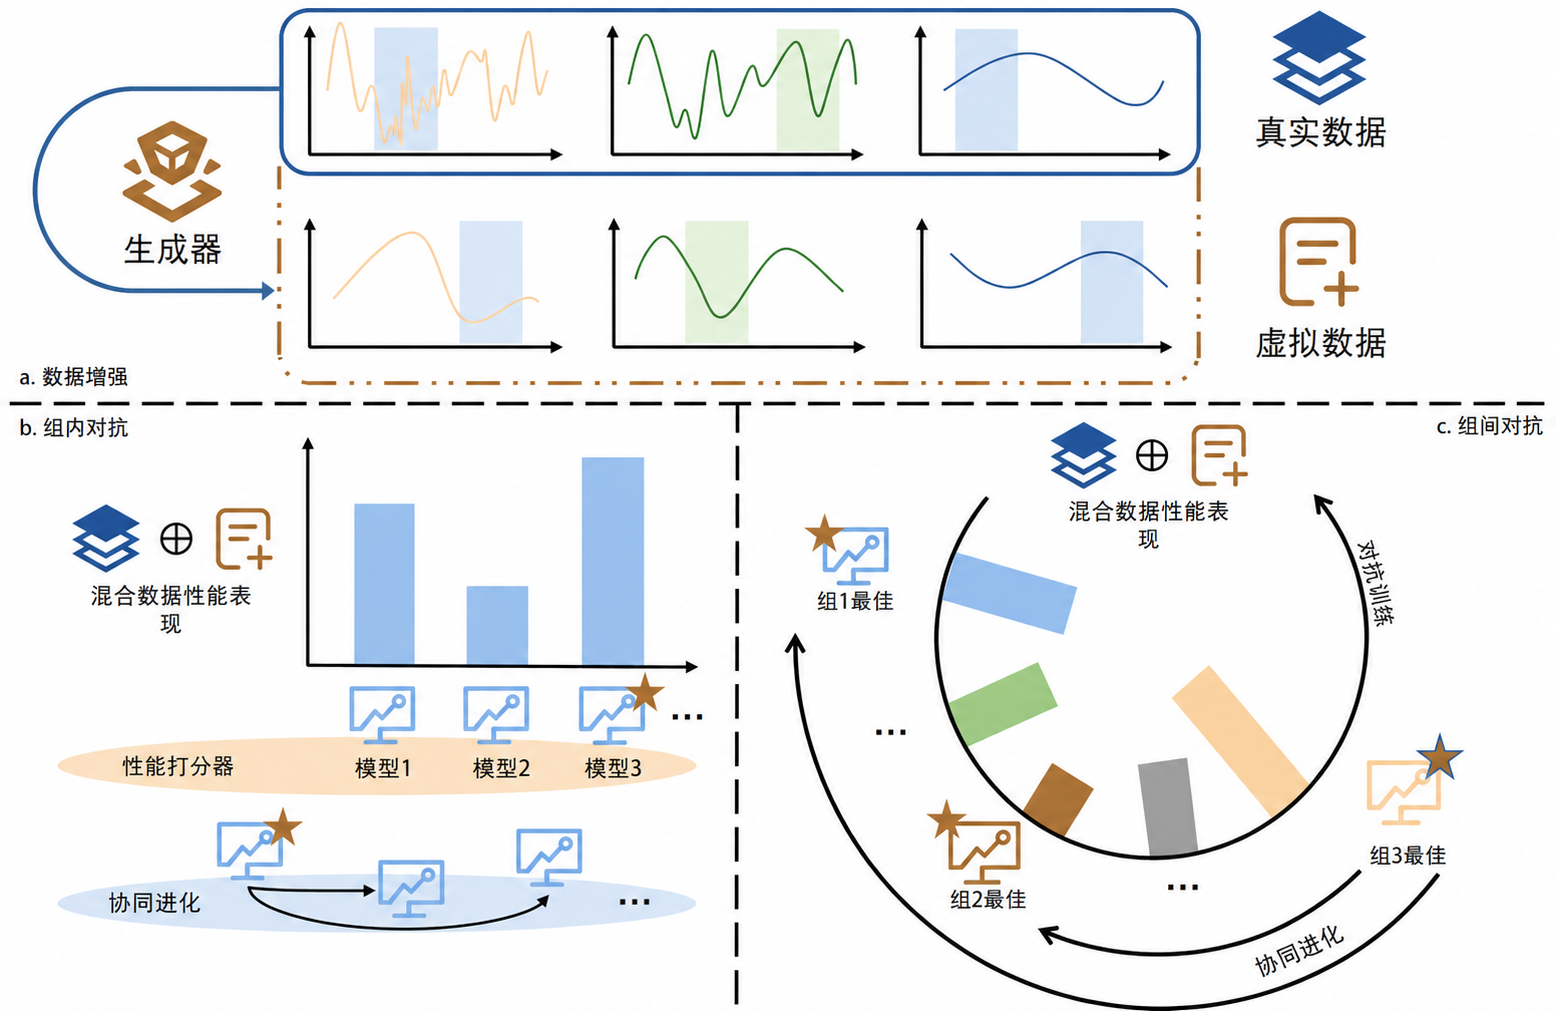
\includegraphics[width=0.85\textwidth]{data/images/highdimframework_cn.png}
\caption{训练策略概览: 监督重构与赛马场训练机制}
% \caption{Overview of Pre-training Strategies: Supervised Reconstruction and 赛马场竞争机制.}

\label{fig:赛马场竞争机制}
\end{figure}


\subsection{过早收敛问题与赛马场竞争机制引入动因}
金融市场数据的高维、高噪与非平稳特征，使得传统时间序列分析难以长期提取稳定表征。在普通训练流程中，模型一旦在某类样本或某组因子上形成早期优势，后续更新往往会继续强化这一优势路径，从而降低对弱幅度但具有解释价值因子的探索能力。本章首先以变分自编码器作为基准表征学习方法，通过压缩与重构学习高维数据中的紧凑表示；在此基础上，引入赛马场竞争机制，将候选模型置于持续评分、竞争、淘汰和迁移的训练过程中。该设计的目的在于，将一次性训练后的静态使用方式转化为动态更新机制，从而缓解高维因子建模中的过早收敛问题。

为检验模型在不同金融任务中的适应性，本章将预测任务划分为三个递进层次。回归任务要求输出连续实数值以逼近未来价格，用于检验模型的精细拟合能力；分类任务关注价格变动方向，用于评估模型对基本方向信息的识别能力；投资任务进一步将未来收益率划分为下跌、平稳和上涨三个区间，使模型输出更接近买入、卖出或观望等交易决策约束。

上述任务组织说明了赛马场竞争机制并非只服务于单一预测目标，而是通过统一的因子表征进入不同层次的金融任务。图~\ref{fig:highdim-task}进一步给出高维金融因子输入、模型组织形式与预测目标之间的对应关系。

\begin{figure}[!htbp]
    \centering 
    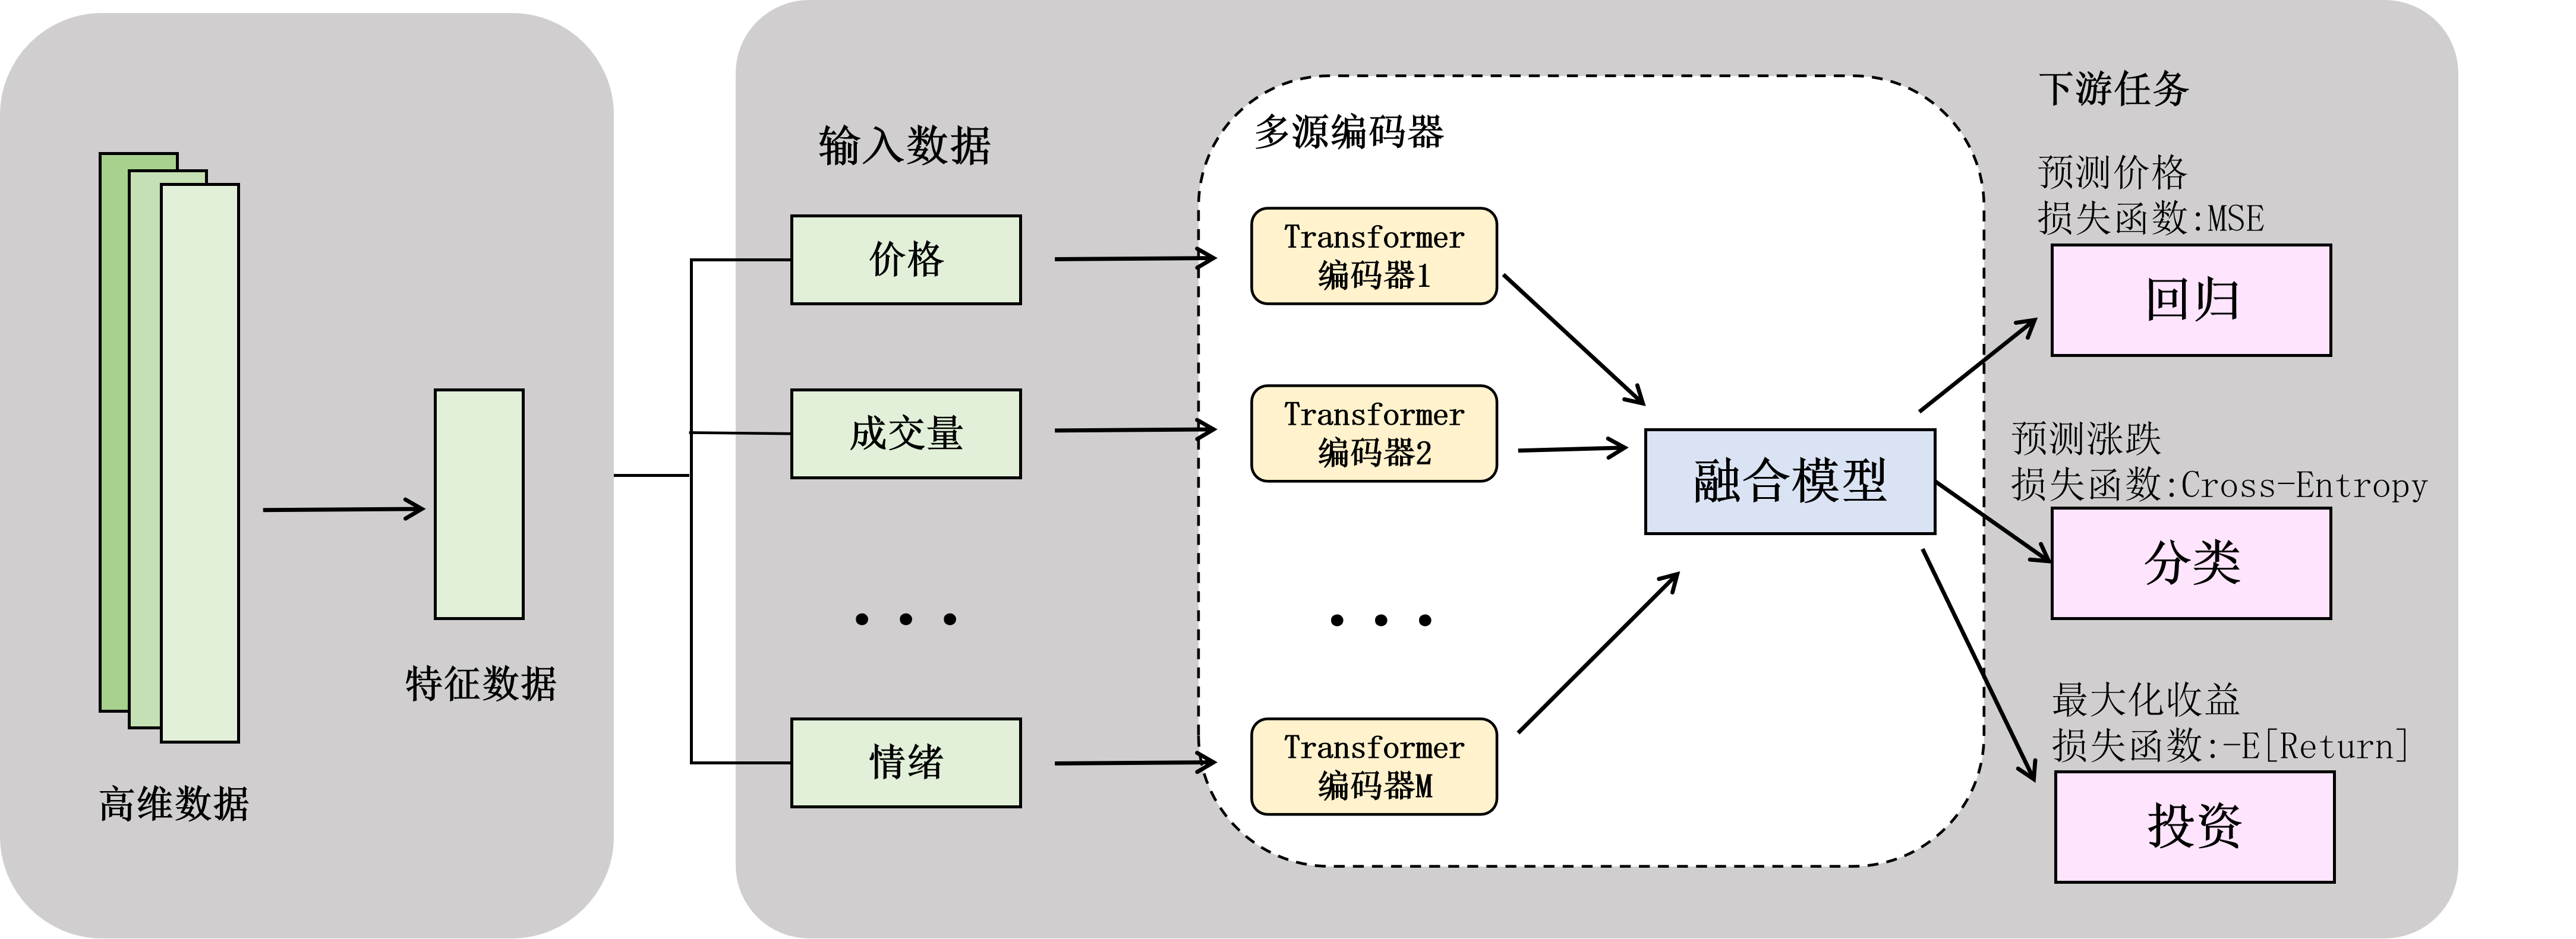
\includegraphics[width=0.8\textwidth]{figures/chap4/高维任务.png} 
    \caption{基于赛马场竞争机制的高维金融因子建模任务}
    \label{fig:highdim-task}
\end{figure}

金融市场数据通常具有高度异构性，不同类型的指标往往反映市场结构的不同侧面，例如基础交易信息刻画流动性与价格行为，技术分析信号揭示趋势与动量，而工程化特征则强调统计结构或潜在风险暴露。图结构半监督学习研究说明，当样本之间存在关系依赖时，显式刻画结构关系有助于提升表示学习效果\cite{kipf2016semi}。这一思想对高维金融因子建模具有启发意义：多源因子并不是简单并列的输入变量，而是可能在资产、时间和市场状态之间形成复杂关联。进一步地，图生成模型研究也表明，复杂结构数据的表示与生成需要同时考虑节点属性和整体结构关系\cite{simonovsky2018graphvae}。因此，在金融因子建模中，若将价量、技术、动量等异构特征直接混合输入同一模型，容易导致特征干扰与表示退化，从而削弱模型对复杂市场动态的刻画能力。

在实际多因子研究中，情绪因子等非价格信息也会被纳入选股与因子组合框架，说明金融特征空间本身具有多源异构属性\cite{ye2023system}。这进一步提示本文，第三章的方法设计不能把所有金融特征视为同质输入，而应先在语义层面区分不同信息来源，再让模型在相对清晰的特征结构上进行竞争和筛选。

基于上述考虑，本章依据语义相关性实施特征分组策略，将输入划分为三个独立组别。第一组为基础价量特征，包括开盘价、最高价、最低价、收盘价和成交量，用于刻画市场运行的基本状态；第二组为技术分析指标，包括移动平均线、平滑异同移动平均线和布林带等，用于描述趋势与波动特征；第三组为动量与随机指标，聚焦相对强弱指数、随机指标等，用于捕捉超买超卖状态及短期反转信号。每一组特征由专用编码器独立处理，以减少不同语义特征之间的相互干扰，并为后续赛马场竞争机制提供更稳定的候选因子表征。

为了消除不同特征量纲之间的差异，我们对每一组特征分别进行了 Z-score 标准化处理。这一步骤保证了每组特征在输入模型时具有相似的分布尺度，从而改善了模型的收敛速度和稳定性。在样本构造方面，我们采用了滑动窗口技术，将时间窗口大小设定为 60 个时间步。这意味着模型将利用过去 60 个交易日的数据来预测未来的市场状态，以覆盖中短期的市场规律。

高维金融数据中充斥着大量噪声，且不同语义类型的特征（如价量、技术指标、动量）在统计性质上存在明显差异。直接在原始空间中进行对抗训练极易导致模式崩溃。为解决这一问题，本阶段引入变分自编码器进行重构预训练，将异构的高维噪声数据映射到一个平滑、连续且去噪的统一潜在空间中，为后续的对抗博弈提供稳定的表征基础。基于不同语义类型的金融特征具有各自独特演化规律的假设，我们构建了一个多编码器融合系统。给定原始输入序列 $X = \{X^{(1)}, X^{(2)}, X^{(3)}\}$，其中 $X^{(k)} \in \mathbb{R}^{B \times T \times D_k}$（$k=1,2,3$）分别对应基础价量特征、技术分析指标与动量随机指标三组特征，$B$ 为批大小，$T$ 为时间步长，$D_k$ 为第 $k$ 组特征维度。

每组特征由独立的 Transformer 编码器 $E^{(k)}_{\phi_k}$ 处理，提取各组的时序表示\cite{vaswani2017attention}：
\begin{equation}
h^{(k)} = E^{(k)}_{\phi_k}(X^{(k)}), \quad h^{(k)} \in \mathbb{R}^{B \times T \times d},
\end{equation}
其中 $d$ 为编码器隐藏维度。随后，三组表示经融合模块 $\mathcal{F}$（注意力机制）整合为统一的潜在表示：
\begin{equation}
h = \mathcal{F}(h^{(1)}, h^{(2)}, h^{(3)}).
\end{equation}

在变分自编码器框架下，融合后的表示经线性映射生成潜变量分布参数：
\begin{equation}
(\mu, \log \sigma^2) = \text{Linear}(h),
\end{equation}
并通过重参数化技巧获得潜变量采样：
\begin{equation}
z = \mu + \sigma \odot \epsilon, \quad \epsilon \sim \mathcal{N}(0, I).
\end{equation}

解码器 $\text{Dec}_{\psi}$ 据此重构原始输入：
\begin{equation}
\hat{X} = \text{Dec}_{\psi}(z).
\end{equation}

训练目标为最大化证据下界，等价于最小化以下损失：
\begin{equation}
\mathcal{L}_{\text{变分自编码器}} = \|X - \hat{X}\|_2^2 + \beta \, D_{\mathrm{KL}}\big(q_\phi(z|X) \,\|\, p(z)\big),
\end{equation}
其中第一项为重构损失，第二项为 库尔贝克—莱布勒散度正则化项，$\beta$ 为平衡系数，$p(z) = \mathcal{N}(0, I)$ 为标准正态先验。库尔贝克—莱布勒散度项迫使后验分布 $q_\phi(z|X)$ 逼近先验分布，使得潜在空间更加平滑连续，避免过拟合并提升泛化能力。

预训练完成后，选择验证集上重构损失最低的模型，保留其编码器 $\{E^{(1)}_{\phi_1}, E^{(2)}_{\phi_2}, E^{(3)}_{\phi_3}, \mathcal{F}\}$ 作为共享表示模块，冻结全部编码器参数，移除解码器。后续所有训练阶段中，输入数据均通过固定编码器映射至潜空间：
\begin{equation}
z = \mathcal{F}\big(E^{(1)}_{\phi_1}(X^{(1)}), E^{(2)}_{\phi_2}(X^{(2)}), E^{(3)}_{\phi_3}(X^{(3)})\big) \in \mathbb{R}^{B \times T \times d_z},
\end{equation}
其中 $d_z$ 为潜在特征维度。对抗训练由此在结构化、去噪的潜空间上进行，而非在高维、噪声充斥的原始特征空间中直接博弈。

经过 $E_{\text{init}}$ 轮独立训练后，所有生成器已具备基本的序列到目标映射能力，为后续对抗训练提供了稳定的初始化基础。

在验证集上对所有生成器和判别器进行全局性能评估，分别识别全局最优与最差的模型：
\begin{equation}
G_{\text{best}} = \arg\min_{G_{i,j} \in \mathcal{G}} \mathcal{L}_{\text{task}}(G_{i,j}), \quad
G_{\text{worst}} = \arg\max_{G_{i,j} \in \mathcal{G}} \mathcal{L}_{\text{task}}(G_{i,j}).
\end{equation}

在完成预训练与对抗式精炼后，模型已能够提取高质量且具备分布感知能力的潜在表示。基于此，我们连接任务特定预测头并进行端到端微调，以适配不同金融应用场景。整体训练流程遵循严格的偏序执行策略：先进行变分自编码器表示学习，再执行赛马场对抗精炼，最后根据任务类型进行下游微调。

\subsection{动态选优规则与模型演化路径}
金融时间序列通常呈现较强的非平稳性与分布漂移特征，直接在高维原始空间中进行对抗训练容易引发收敛不稳定与模式崩溃。本章采用“先表征、后赛马”的多阶段训练方式：先通过变分自编码器重构预训练提取结构化潜在表示，再进行多生成器独立预热以建立基线预测能力，随后在潜在空间中引入群组交叉对抗（GCA）作为辅助的交叉校验环节，最后由赛马场竞争机制实施动态评分、末位淘汰与知识蒸馏。需要强调的是，GCA在本章中并不是主体方法，而是为赛马场竞争提供分布反馈和模型差异校验；本章的核心仍是通过持续竞争和知识迁移抑制过早收敛。该路径旨在使后续竞争过程建立在相对稳定的潜空间之上，降低早期对抗训练直接拟合复杂分布带来的震荡。

为展示高维金融因子建模框架的训练逻辑，本节将上述过程整理为形式化算法流程。整个训练过程按照固定阶段顺序执行：先进行表示学习（变分自编码器预训练），再执行交叉对抗校验与赛马场竞争，最后根据任务类型进行下游微调。

图~\ref{fig:HIGHDIM-workflow}对应展示这一训练流程中的关键步骤，使后续算法描述能够与全局评估、学生模型培养、末位淘汰替换和对齐训练等环节保持对应。

\begin{figure}[!htbp]
    \centering
    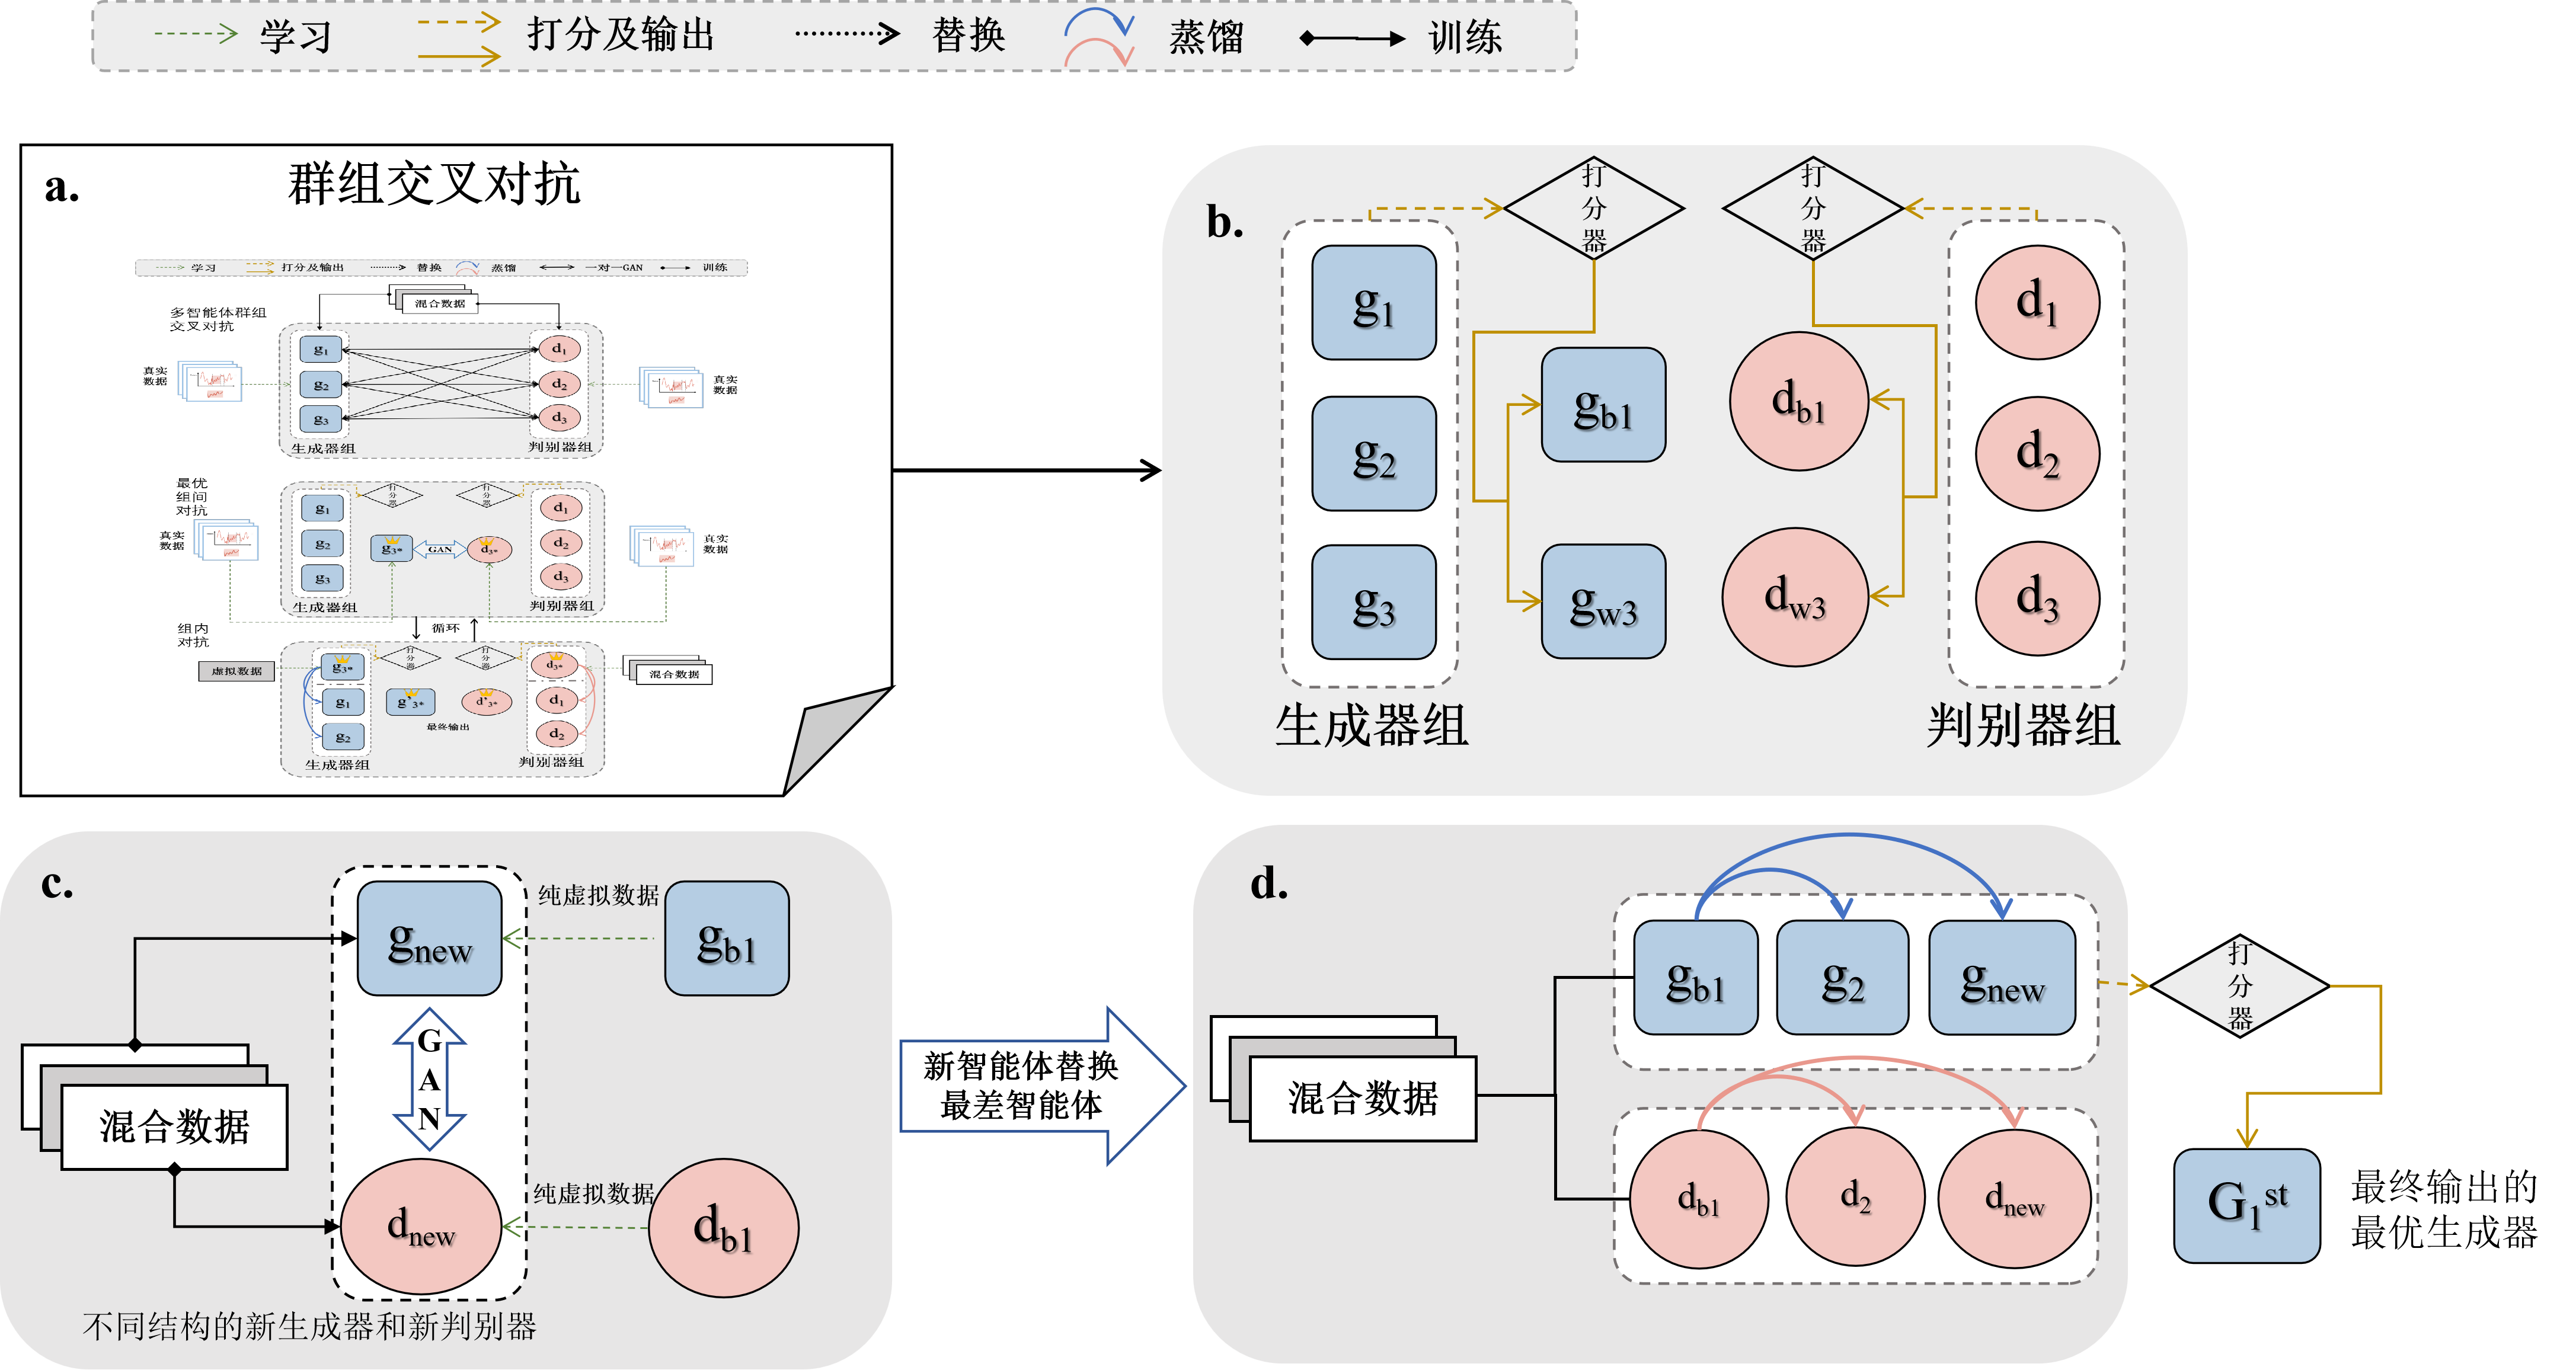
\includegraphics[width=0.8\textwidth]{figures/chap4/赛马场对称.png}
    \caption{赛马场训练流程示意图}
    \label{fig:HIGHDIM-workflow}
\end{figure}

\begin{algorithm}[H]
\caption{高维因子建模框架总体训练流程}
\label{alg:highdim_overall}
\begin{algorithmic}[0]
\Require 原始特征序列 $X \in \mathbb{R}^{T \times D_{\text{raw}}}$，特征分组列表 $\mathcal{F}_1, \ldots, \mathcal{F}_K$；超参数：$N_{\text{VAE}}$（变分自编码器预训练轮数），$N_{\text{GCA}}$（对抗训练轮数），$N_{\text{RT}}$（赛马场竞争机制训练轮数），$\lambda_{\text{adv}}$（对抗权重），$\delta$（投资阈值），$\lambda$（误差罚项）
\Ensure 训练好的生成器 $G^{\star}$，最优判别器 $D^{\star}$，各任务的预测头 $\phi_{\text{reg}}, \phi_{\text{cls}}, \phi_{\text{inv}}$
\Statex
\State \textbf{/* 阶段 1：变分自编码器表示预训练 */}
\State $Z \leftarrow \text{变分自编码器预训练}(X; \theta_E, \theta_D)$ \Comment{学习潜在表示 $Z \in \mathbb{R}^{T \times d_{\text{model}}}$}
\State $E \leftarrow \text{Freeze}(E)$ \Comment{冻结编码器，用于下游特征提取}
\Statex
\State \textbf{/* 阶段 2：交叉对抗校验与赛马场竞争 */}
\State 初始化生成器组 $\mathcal{G} = \{G_1, \ldots, G_N\}$ 和判别器组 $\mathcal{D} = \{D_1, \ldots, D_M\}$
\State $\mathcal{G}, \mathcal{D} \leftarrow \text{执行赛马场竞争机制}(\mathcal{G}, \mathcal{D}, Z)$ \Comment{见算法 \ref{alg:highdim_mgca_detail}}
\Statex
\State \textbf{/* 阶段 3：下游任务微调 */}
\State 连接任务特定预测头：$\phi_{\text{reg}}$（回归头），$\phi_{\text{cls}}$（分类头），$\phi_{\text{inv}}$（投资头）
\State 在 $Z$ 上分别微调各预测头，最小化对应任务损失
\Statex
\State \Return $\mathcal{G}, \mathcal{D}, \phi_{\text{reg}}, \phi_{\text{cls}}, \phi_{\text{inv}}$
\end{algorithmic}
\end{algorithm}

\begin{algorithm}[H]
\caption{赛马场竞争与交叉校验详细流程}
\label{alg:highdim_mgca_detail}
\begin{algorithmic}[0]
\Require 潜在表示序列 $Z \in \mathbb{R}^{T \times d_{\text{model}}}$，混合比例 $1-\alpha$（真实数据），生成器组 $\mathcal{G}$，判别器组 $\mathcal{D}$，打分阈值 $\theta_{\text{score}}$
\Ensure 最优生成器 $G^{\star}$，最优判别器 $D^{\star}$
\Statex
\State \textbf{/* Stage 1：生成器预训练 */}
\For{轮次 $\in \{1, \ldots, N_{\text{VAE}}\}$}
    \State $\mathcal{L}_{\text{VAE}} \leftarrow \text{ELBO}(G_{\text{VAE}}(x), x)$
    \State 使用 $\mathcal{L}_{\text{VAE}}$ 更新 $G_{\text{VAE}}$ 和 $E$
\EndFor
\Statex
\State \textbf{/* Stage 2：混合数据生成 */}
\State $\tilde{Z} \leftarrow G_{\text{VAE}}(Z)$ \Comment{生成器输出虚拟潜在序列}
\State $Z_{\text{mixed}} \leftarrow \alpha \cdot Z \oplus (1-\alpha) \cdot \tilde{Z}$ \Comment{按比例混合}
\Statex
\State \textbf{/* Stage 3：组内对抗与蒸馏 */}
\For{每组判别器 $\mathcal{D}^{(g)}$}
    \State 在 $Z_{\text{mixed}}$ 上并行训练组内所有判别器
    \State 在 $\mathcal{D}_{\text{val}}$ 上评估，选出组内最优 $D_g^{\star}$（交叉熵最小）
    \For{组内每个判别器 $D_k \neq D_g^{\star}$}
        \State $\mathcal{L}_{\text{distill}} \leftarrow \text{MSE}(\text{Feat}_{D_k}, \text{Feat}_{D_g^{\star}}) + \text{MSE}(\text{Logits}_{D_k}, \text{Logits}_{D_g^{\star}})$
        \State 使用 $\mathcal{L}_{\text{distill}}$ 更新 $D_k$
    \EndFor
\EndFor
\Statex
\State \textbf{/* Stage 4：组间蒸馏与新学生竞争 */}
\State 从所有 $D_g^{\star}$ 中选出全局最优 $D^{\star}$ 和最差 $D^{\dagger}$
\State 实例化新学生判别器：$D_{\text{new}} \leftarrow \text{DeepCopy}(D^{\star})$
\State 在 $Z_{\text{mixed}}$ 上训练 $D_{\text{new}}$：蒸馏所有判别器的平均表现
\State $D^{\dagger} \leftarrow D_{\text{new}}$ \Comment{替换最差判别器}
\Statex
\State \Return $G_{\text{VAE}},\; D^{\star}$
\end{algorithmic}
\end{algorithm}

\begin{algorithm}[H]
\caption{下游任务推理与信号生成}
\label{alg:highdim_inference}
\begin{algorithmic}[0]
\Require 当前时刻特征窗口 $x_t \in \mathbb{R}^{W \times D_{\text{raw}}}$，训练好的生成器 $G^{\star}$，变分自编码器编码器 $E$，各任务预测头 $\phi_{\text{reg}}, \phi_{\text{cls}}, \phi_{\text{inv}}$，置信度阈值 $c_{\min}$
\Ensure 交易信号 $a_t \in \{-1, 0, +1\}$，动态权重 $w_t$
\Statex
\State \textbf{/* 步骤 1：潜在表示提取 */}
\State $z_t \leftarrow E(x_t) \in \mathbb{R}^{d_{\text{model}}}$
\Statex
\State \textbf{/* 步骤 2：回归预测 */}
\State $\hat{r}_t^{\text{reg}} \leftarrow \phi_{\text{reg}}(G^{\star}(z_t))$
\Statex
\State \textbf{/* 步骤 3：分类预测 */}
\State $\hat{y}_t^{\text{cls}} \leftarrow \phi_{\text{cls}}(G^{\star}(z_t)) \in \{0, 1, 2\}$ \Comment{下跌/中性/上涨}
\Statex
\State \textbf{/* 步骤 4：投资决策（若启用） */}
\State $a_t^{\text{inv}} \leftarrow \phi_{\text{inv}}(G^{\star}(z_t)) \in \{0, 1, 2\}$
\Statex
\State \textbf{/* 步骤 5：多资产动态权重（回归任务） */}
\State $c_t \leftarrow \text{置信度}(G^{\star}(z_t))$ \Comment{softmax 输出的最大概率}
\State $R_t \leftarrow \sum_{\tau=1}^{t} \hat{r}_{\tau}^{\text{reg}}$ \Comment{累积预测收益率}
\State $S_t \leftarrow \dfrac{(2.5 \cdot c_t - 1) \cdot R_t}{1 + \lambda \cdot \text{MSE}_{\text{val}}}$
\State $w_i \leftarrow \dfrac{|S_i|}{\sum_j |S_j|}$ \Comment{绝对值归一化权重}
\State $L_i \leftarrow \dfrac{\text{TotalEquity} \cdot |w_i|}{P_i \cdot \text{Mult}_i \cdot \text{Margin}_i}$ \Comment{保证金手数}
\Statex
\State \Return $(a_t^{\text{cls}}, a_t^{\text{inv}}), \; S_t, \; L_i$
\end{algorithmic}
\end{algorithm}

传统的单一生成器—判别器架构在面对非平稳金融时间序列时，往往只能拟合局部数据分布。为避免候选模型在进入赛马场竞争之前已经形成过强的单一路径依赖，本框架在预热之后引入群组交叉对抗（GCA）作为辅助校验阶段。该机制通过一对多、组内与组间的交互训练，使不同架构的生成器在相互约束中形成差异化预测策略。同时构建 $N_D$ 组条件判别器 $\mathcal{D} = \{D_{k,l}\}$，与生成器群体进行多轮对抗训练：一方面扩展判别反馈来源，另一方面在组内进行性能评估与知识蒸馏，使落后成员向优势成员对齐。经过这一阶段后，生成器与判别器形成相对稳定的交互关系，为后续赛马场竞争机制中的动态淘汰与演化更新提供基础。

在群组交叉对抗完成后，模型群体只获得了初步的分布校验和差异化约束，并不意味着因子表征已经完成动态筛选。本框架进一步引入赛马场竞争机制进行动态淘汰与精炼。即使模型群体保持一定多样性，长时间静态训练后仍可能集中到单一优势路径，导致面对新市场状态时泛化能力下降。赛马场竞争机制通过周期性的全局评估、学生模型培养与末位淘汰替换，引入新的参数起点并淘汰表现不足的成员，使模型群体在持续更新中保持探索能力。由此，GCA承担前置交叉校验功能，赛马场竞争机制承担持续选优、替换和知识迁移功能，二者在训练流程中形成前后衔接而非并列替代关系。

创建全新初始化的学生生成器 $G_s$ 与学生判别器 $D_s$，通过交替执行对抗训练与知识蒸馏进行培养。学生判别器向全局最优判别器 $D_{\text{best}}$ 学习，蒸馏损失涵盖 logits 对齐、概率分布对齐与中间层特征对齐三个层面：
\begin{equation}
\mathcal{L}_{D_s}^{\text{distill}} = \lambda_{\text{feat}}\big(\|o_s - o_t\|_2^2 + \|\sigma(o_s) - \sigma(o_t)\|_2^2 + \|f_s - f_t\|_2^2\big).
\end{equation}
学生生成器向全局最优生成器 $G_{\text{best}}$ 学习，总损失结合蒸馏、对抗与重构三项：
\begin{equation}
\mathcal{L}_{G_s}^{\text{distill}} = \lambda_d \cdot \|G_s(z) - G_{\text{best}}(z)\|_2^2 + \lambda_{\text{adv}} \cdot \ell_{\text{二元交叉熵}}(D_s(z, G_s(z)), \mathbf{1}) + \mathcal{L}_{\text{task}}(G_s(z), y).
\end{equation}


训练完成后，执行末位淘汰替换：$G_{\text{worst}} \leftarrow G_s,\; D_{\text{worst}} \leftarrow D_s$，同时重置被替换位置的优化器状态。替换完成后，所有生成器—判别器对进入局部对抗校验训练，并同时通过蒸馏损失向全局最优生成器 $G_{\text{best}}$ 的输出对齐：
\begin{equation}
\mathcal{L}_{G_{i,j}}^{\text{align}} = \mathcal{L}_{\text{task}}(\hat{y}_{i,j}, y) + \lambda_{\text{adv}} \cdot \mathcal{L}_{\text{adv}}^{(i,j)} + \lambda_d \cdot \|\hat{y}_{i,j} - G_{\text{best}}(z)\|_2^2.
\end{equation}
赛马场竞争机制通过“评估—培养—淘汰—对齐”的循环过程，使模型群体在竞争筛选与协作蒸馏中持续调整，其效果主要体现在非平稳数据下的泛化表现和训练稳定性上。

动态选优规则主要解决“谁更适合当前市场状态”的评价问题；若缺少跨阶段知识继承和反向校正，模型群体仍可能在若干轮筛选后集中到单一优势路径。因此，后续的成熟—新生模型双向知识迁移机制，是赛马场竞争机制能够持续演化而不退化为静态集成的关键环节。

本章的损失函数设计主要包含任务损失、对抗损失与蒸馏损失三类，分别对应不同任务的特性和对抗训练的需求。对于回归任务，我们设计了金融感知重构损失，对开盘价、最高价、最低价、收盘价与成交量五个核心维度赋予特定权重：
\begin{equation}
\mathcal{L}_{\text{financial}} = w_{\text{price}} \cdot \frac{1}{4} \sum_{k \in \{O,H,L,C\}} \text{均方误差}(y_k, \hat{y}_k) + w_{\text{vol}} \cdot \text{均方误差}(y_V, \hat{y}_V)
\end{equation}
其中 $w_{\text{price}}$ 和 $w_{\text{vol}}$ 分别为价格类特征和成交量特征的权重（默认分别设为1.0和0.8）。对于分类任务，使用标准交叉熵损失；对于投资任务，采用严格的阈值法生成真实标签 $y_{\text{inv}}$，设定阈值 $\delta$（默认0.02），将连续收益率映射为做空/持有/做多三类决策，同样使用交叉熵损失优化。对抗损失定义为生成样本在判别器眼中的二元交叉熵损失，蒸馏损失通过均方误差衡量学生模型与最优教师模型输出之间的差异，实现跨代知识传递。

\subsection{模型预热与公平竞争约束}
在完成变分自编码器重构预训练、获得结构化潜在表示后，本框架进一步对多个生成器进行独立预热，以消除对抗训练初期的“冷启动”问题。
在对抗训练的早期阶段，如果生成器和判别器均从零开始随机初始化，极易陷入梯度震荡或导致生成器被判别器迅速压制，从而丧失探索能力。本阶段实施多生成器独立预热机制，在不引入对抗信号的情况下，仅通过任务损失为所有生成器建立基本的序列到目标映射能力，确保它们在进入后续对抗训练前具备合格的基线预测水平。我们构建 $N_G$ 组生成器，每组包含 $P$ 个成员，记为 $\mathcal{G} = \{G_{i,j}\}_{i=1,\ldots,N_G;\, j=1,\ldots,P}$。为保障架构多样性，组内成员采用异构网络结构（门控循环单元、长短期记忆网络、Transformer架构 交替分配），使不同生成器能够从不同的归纳偏置出发探索数据分布。

每个生成器接受潜在特征 $z$ 作为输入，输出预测值 $\hat{y}_{i,j} = G_{i,j}(z)$。预热阶段仅使用任务损失进行独立训练，不引入对抗信号：
\begin{equation}
\mathcal{L}_{\text{pretrain}}^{(i,j)} = \mathcal{L}_{\text{task}}(\hat{y}_{i,j},\, y),
\end{equation}
其中 $\mathcal{L}_{\text{task}}$ 根据任务类型定义：回归任务使用均方误差，分类与投资任务使用交叉熵损失。对于回归任务，当目标列包含开盘价、最高价、最低价、收盘价与成交量五个维度时，进一步采用金融感知重构损失，对价格维度和成交量维度分别赋予不同权重。

公平竞争约束为后续知识迁移提供了统一的评价基础。只有在所有候选模型按照相同任务损失、相同验证规则和相同对抗约束进行比较时，成熟模型的经验边界与新生模型的差异化反馈才具有可比性。由此，动态选优规则、公平竞争约束与双向知识迁移共同构成赛马场竞争机制的主要训练环节。

\subsection{成熟—新生模型的双向知识迁移机制}
在赛马场竞争机制中，成熟模型与新生模型不只是替换关系，而是动态演化过程中的两类功能角色。成熟模型指在当前评分规则下已经获得相对稳定表现的候选模型，其优势在于能够提供较高质量的特征表达和预测基准；新生模型则指在训练过程中被重新初始化或引入的候选模型，其作用在于为模型群体提供新的参数起点、结构扰动和探索方向。若只保留成熟模型，系统容易沿已有优势路径过早收敛；若只依赖新生模型，训练过程又会缺乏稳定的知识继承。因此，本章将二者之间的关系设计为双向知识迁移过程，以在稳定性与探索性之间取得平衡。

成熟模型向新生模型的知识迁移主要用于降低新生模型的冷启动成本。在动态选优规则确定当前优势模型后，系统可将成熟模型的输出分布、特征表示或任务损失方向作为软约束，引导新生模型在训练初期快速接近有效解空间。该过程并不要求新生模型完全复制成熟模型，而是利用成熟模型提供的经验边界，使新生模型在保持结构差异的同时避免无效搜索，从而提高因子建模阶段的训练效率。

新生模型向成熟模型的反向迁移则用于抑制成熟模型的路径固化。当新生模型在某些局部市场状态、特定因子组合或异常波动区间中表现出更优的适应性时，其输出差异不应被简单视为噪声，而应被纳入成熟模型的校正信息。通过将新生模型的有效偏差信号反馈给成熟模型，系统能够迫使成熟模型重新审视已形成的特征依赖关系，降低其对单一优势因子或历史局部模式的过度依赖。

由此，成熟—新生模型的双向知识迁移机制形成了“稳定继承—差异探索—反向校正”的循环过程。成熟模型保证群体演化不偏离已有高性能区域，新生模型维持模型空间的探索能力，二者在统一评分规则和公平竞争约束下共同作用，使赛马场竞争机制不仅能够完成优胜劣汰，还能够延迟单一模型的过早收敛，提升高维金融因子表示在非平稳市场环境下的鲁棒性。

\section{实验}

\subsection{实验数据集}
为检验赛马场竞争方法在高维金融因子建模任务中的表现，本章构建了覆盖多品种、多任务的实验基准。该平台涵盖4大板块（农业、能源、金属、化工）、16种期货品种（棉花、豆粕、玉米、白糖、动力煤、原油、甲醇、焦炭、铜、黄金、热卷、铁矿石、螺纹钢、PP、PTA、PVC），涉及回归、分类和投资三种下游任务范式。实验同时在单资产和多资产组合两个维度上进行验证，共构建10个资产组别（见表\ref{tab:highdimassetGrouping}），以覆盖单一品种、板块内组合、跨板块组合和全市场组合等不同因子结构。所有实验均基于200万元初始资本，回测时间跨度覆盖超过500个交易日。

本章实验不仅比较策略收益高低，也检验赛马场竞争方法是否能够在不同资产、任务和市场状态下改善高维金融因子表征的稳定性、有效性和样本外适应能力。因此，后续分析同时关注收益率、最大回撤、训练误差、分类准确率和跨组一致性等指标，以观察动态选优、末位淘汰与知识迁移对高维因子建模过程的影响。

\begin{table}[!htbp]
\centering
\caption{资产分组配置详情}
\label{tab:highdimassetGrouping}
\small
\setlength{\tabcolsep}{4pt}
\renewcommand{\arraystretch}{1.15}
\begin{tabular}{>{\raggedright\arraybackslash}p{2.4cm} >{\centering\arraybackslash}p{2.4cm} >{\raggedright\arraybackslash}p{7.8cm}}
\toprule
类别 & 资产组别 & 包含资产 \\
\midrule
农业 & 板块组 & 玉米、豆粕、棉花、白糖 \\
\addlinespace
能源 & 板块组 & 原油、动力煤、甲醇 \\
\addlinespace
金属 & 板块组 & 铜、黄金、铁矿石、焦炭、热卷、螺纹钢 \\
\addlinespace
化工 & 板块组 & PTA、PP、PVC \\
\addlinespace
跨板块 & 跨板块小组合 & 铜、黄金、原油 \\
\addlinespace
跨板块 & 跨板块大组合 & 铜、黄金、原油、玉米、豆粕、棉花 \\
\addlinespace
全市场 & 全品种组合 & 全部16种期货品种 \\
\bottomrule
\end{tabular}
\end{table}

以上资产分组覆盖单一品种、板块组合、跨板块组合与全市场组合，能够用于检验赛马场竞争方法在不同因子结构和市场状态下的适应性。

\subsection{实验设计}
本章采用与赛马场竞争机制完全相同网络架构、但未启用动态竞争机制的标准训练模型作为对照组，并通过基于历史数据的滚动回测流程评估赛马场竞争机制带来的增量作用。实验设计的核心目的，是检验动态选优、末位淘汰和知识迁移是否能够改善高维因子表征，而不是仅比较单一模型在某一指标上的局部优劣。

本章实验采用统一的对照框架，将启用赛马场竞争机制的模型与未启用该机制的基准模型进行比较。两类模型保持相同的特征输入、任务划分、网络骨干和回测区间，差异仅在于是否引入动态选优、末位淘汰、知识蒸馏与成熟—新生模型双向知识迁移。通过这种控制变量方式，可以将性能差异主要归因于赛马场竞争机制本身，而不是数据划分、模型容量或任务定义的变化。

为避免单一指标造成误判，实验从训练阶段和回测阶段两个层面展开。训练阶段主要观察均方误差、分类准确率以及不同资产组之间的表现差异，用于判断赛马场竞争方法是否改善因子表征学习过程；回测阶段则关注收益率、最大回撤和最终净值等指标，用于判断被筛选出的因子表征是否能够转化为更稳健的交易表现。该设计与本章的机制定位保持一致，即从多个维度考察赛马场竞争机制对高维金融因子建模的影响。

\subsection{结果分析与讨论}
本节在前述统一对照框架下，从胜率统计、收益凸性、任务类型差异和典型案例四个层面分析赛马场竞争机制的实验表现。基准模型与赛马场竞争机制采用相同的网络结构，区别在于基准模型不启用动态淘汰与进化精炼机制，而采用标准训练流程。稳健动态资产组合研究表明，在市场状态变化和估计误差同时存在时，模型需要通过稳健约束或动态调整机制降低风险暴露的不稳定性\cite{zhu2007robust}。因此，本节不只比较策略收益率，也同时观察最大回撤、夏普比率（Sharpe Ratio）和卡玛比率（Calmar Ratio）等风险调整指标，以判断赛马场竞争机制是否真正改善了高维金融因子建模质量。

在结果解释上，本章避免仅以单个收益指标判断模型优劣。若动态淘汰和知识迁移能够在部分市场中降低回撤、减少极端误判或改善亏损状态，可以说明该机制在高维金融因子建模中具有一定的优化价值；若在部分板块中出现收益下降，也应被理解为机制适用边界的体现，不能简单视为整体失效。基于这一口径，后文依次从整体胜率、收益凸性、任务类型差异和典型品种表现展开分析。

首先，从收益分布和任务差异看，赛马场竞争机制并不是在所有场景中均匀提高收益，而是在部分市场状态下形成较强的上行弹性。获胜案例的平均改进幅度（+98.7％）在绝对值上明显高于败北案例的平均降幅（-62.3％），凸性比率达1.58。在赛马场竞争机制获胜的18个案例中，有7个属于“亏损转盈利”场景，即基准模型产生亏损而赛马场竞争机制实现盈利。以200万元初始资本为基准，Top 10盈利案例合计贡献了超过+630万元的超额利润，其中棉花回归任务单项即贡献了+255.5万元的超额利润。

为了观察超额利润的来源分布，图~\ref{fig:highdimprofitwaterfall}将Top 10盈利案例与Top 5亏损案例的绝对利润影响放在同一尺度下比较。该图主要用于判断正向案例的利润贡献是否能够覆盖负向案例带来的损失，而不是简单展示单个案例的收益高低。
进一步看，图~\ref{fig:highdimtopimprovements}列出了Alpha生成最佳案例（Top 10）。这些案例用于补充说明：赛马场竞争机制的优势并不平均分布于所有资产，而是在部分高维因子关系更易被动态筛选的市场状态中集中体现，其中棉花以340\%的提升幅度位居榜首。

\begin{figure}[!htbp]
    \centering 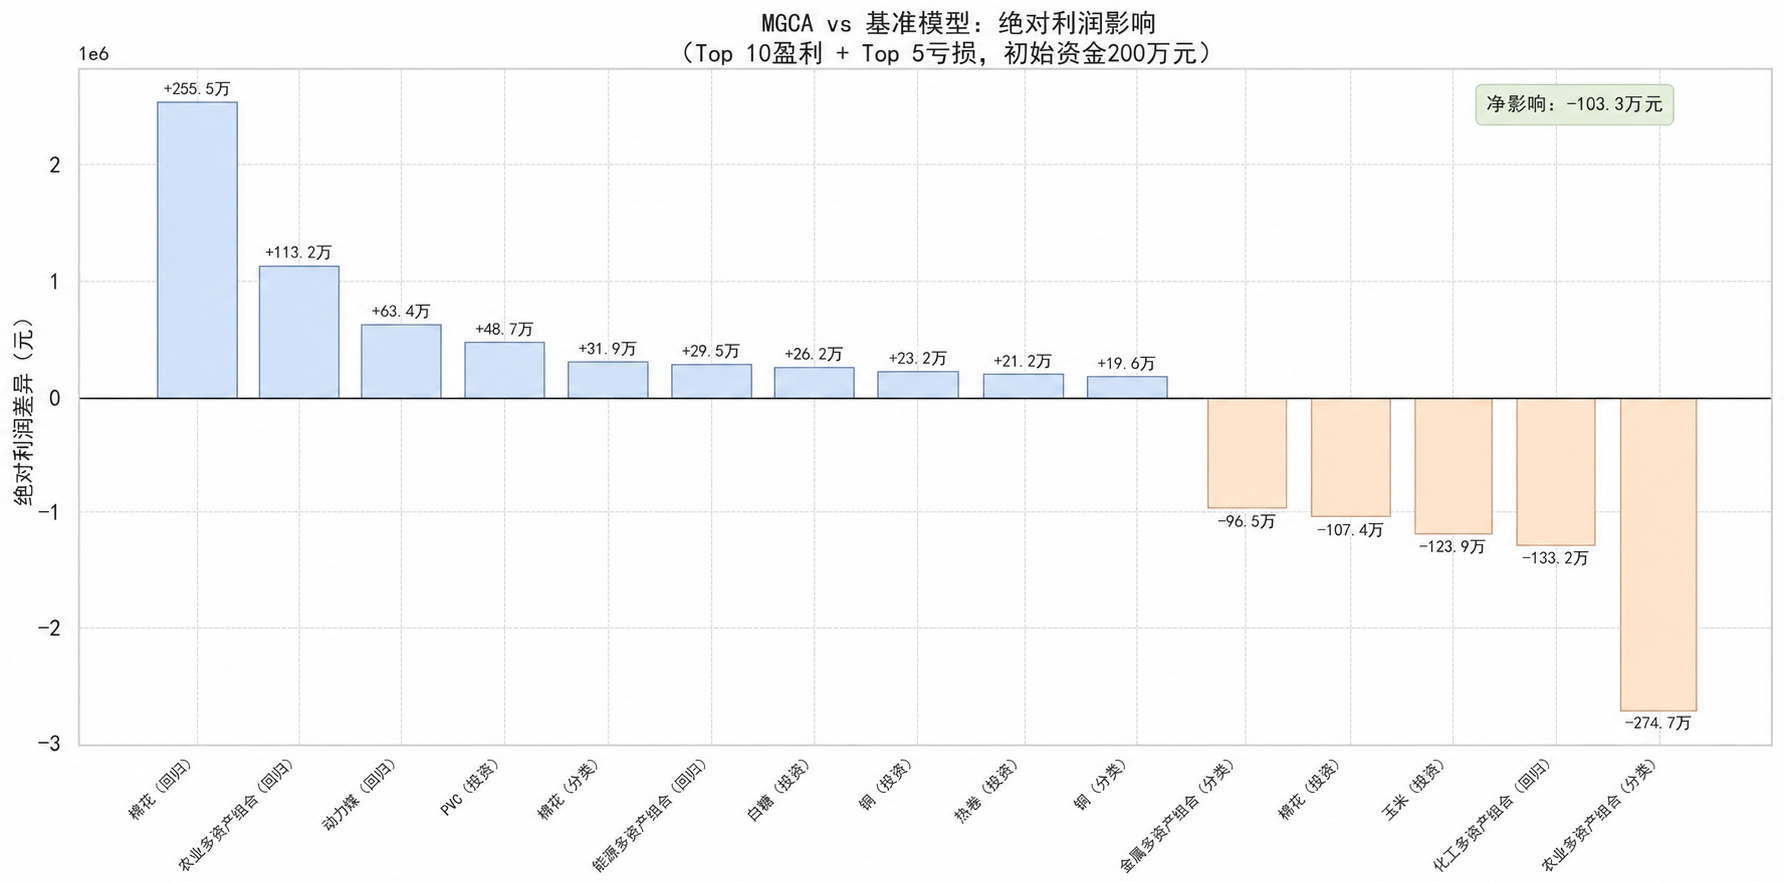
\includegraphics[width=0.8\textwidth]{figures/chap4/fig19_profit_waterfall_cn.png} 
    \caption{绝对利润影响瀑布图（Top 10盈利案例与Top 5亏损案例）}
    \label{fig:highdimprofitwaterfall}
\end{figure}



\begin{figure}[!htbp]
    \centering 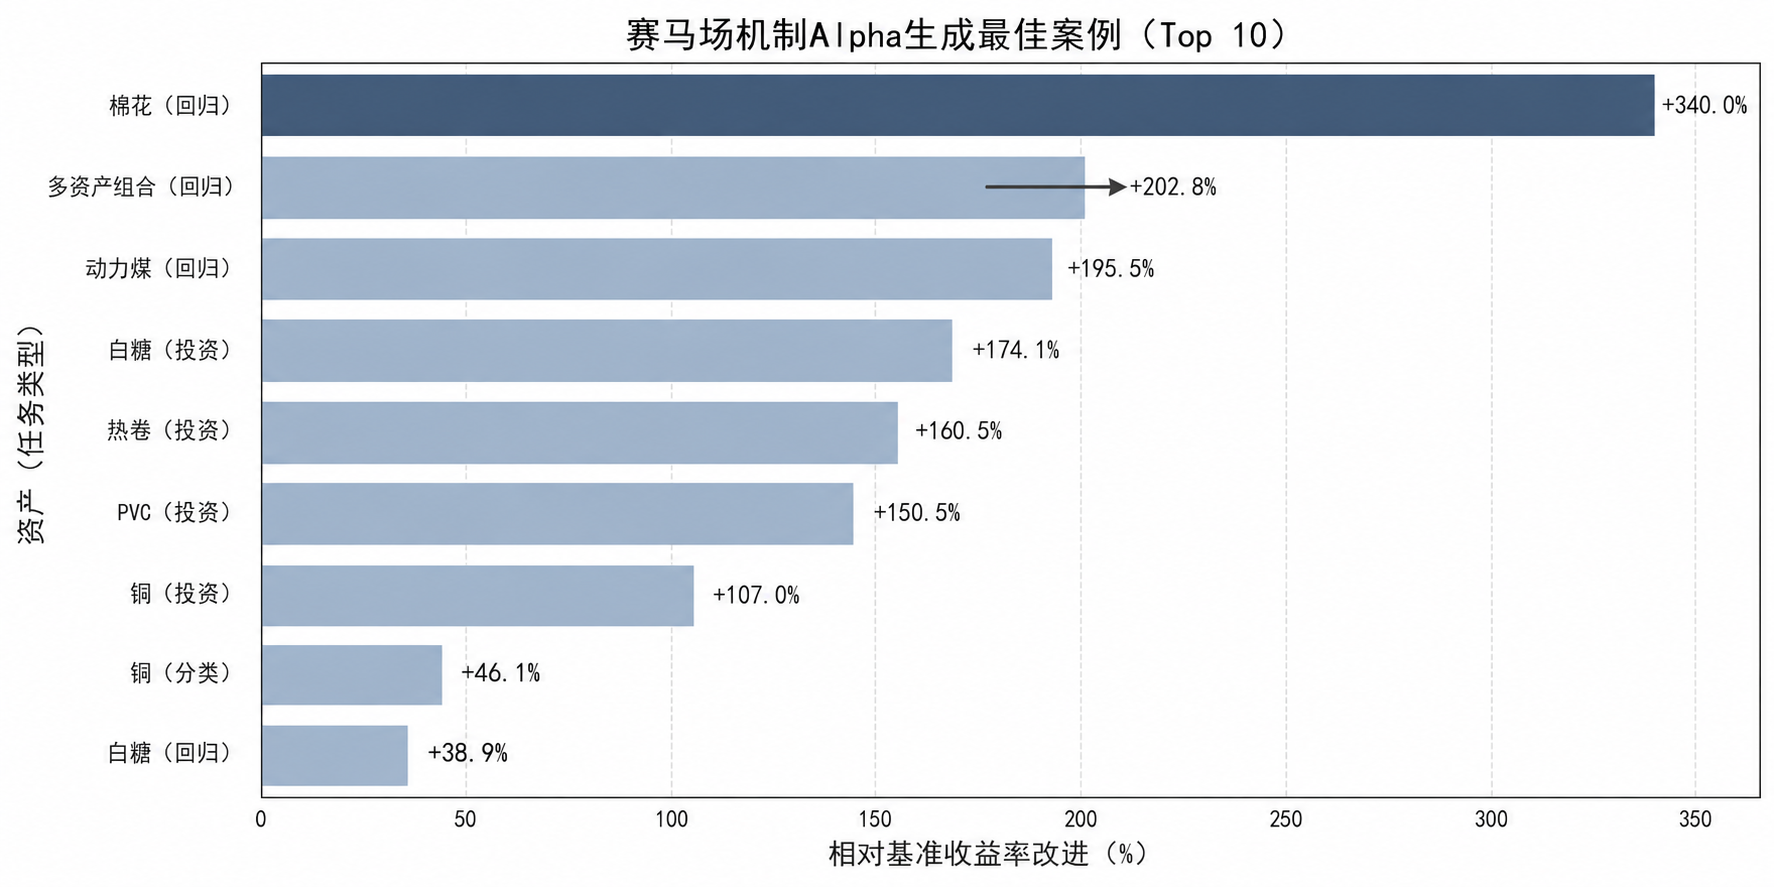
\includegraphics[width=0.8\textwidth]{figures/chap4/fig3_top_improvements_cn.png} 
    \caption{Alpha生成最佳案例（Top 10）}
    \label{fig:highdimtopimprovements}
\end{figure}

从收益改进分布看，图~\ref{fig:highdimreturnDistribution}呈现出明显的右偏长尾特征，尾部包含棉花（+340\%）、能源多资产（+202\%）等正向案例。这说明赛马场竞争机制并非简单提高所有样本的平均表现，而是在部分市场状态下捕捉到收益改善机会。

\begin{figure}[!htbp]
    \centering 
    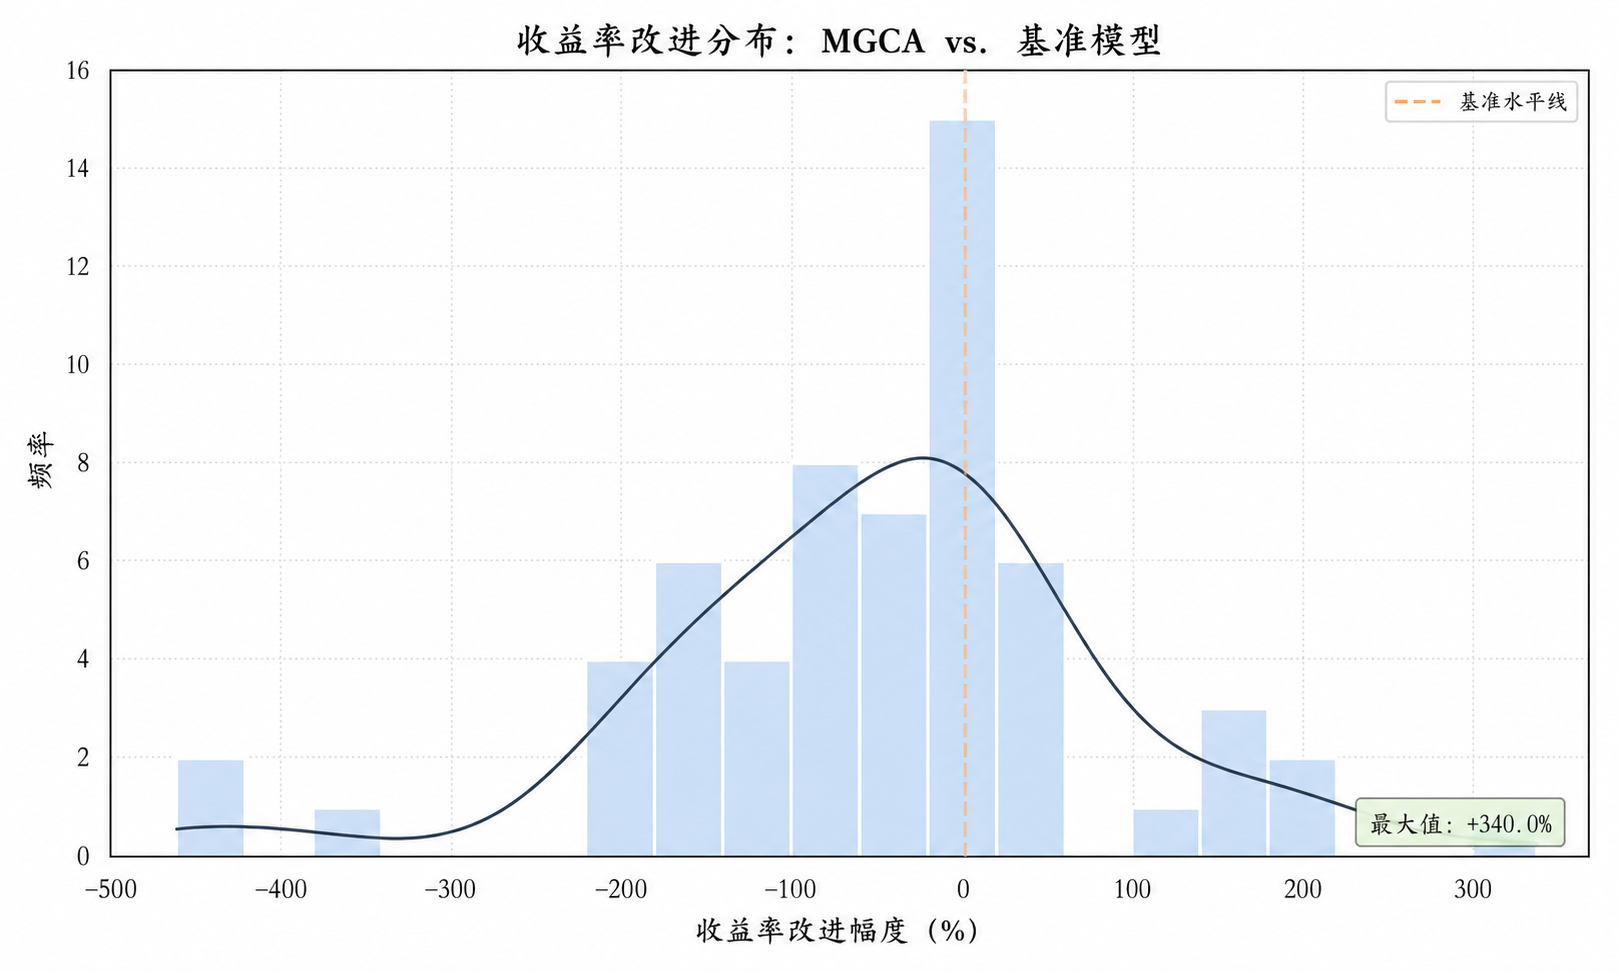
\includegraphics[width=0.8\textwidth]{figures/chap4/fig1_return_distribution_cn.png} 
    \caption{收益率改进分布直方图}
    \label{fig:highdimreturnDistribution}
\end{figure}

任务类型差异进一步说明了该机制的适用场景。图~\ref{fig:highdimtaskcomp}比较了不同任务类型下的平均收益改进幅度，用于判断赛马场竞争机制更容易在哪类预测目标中发挥作用。

\begin{figure}[!htbp]
    \centering 
    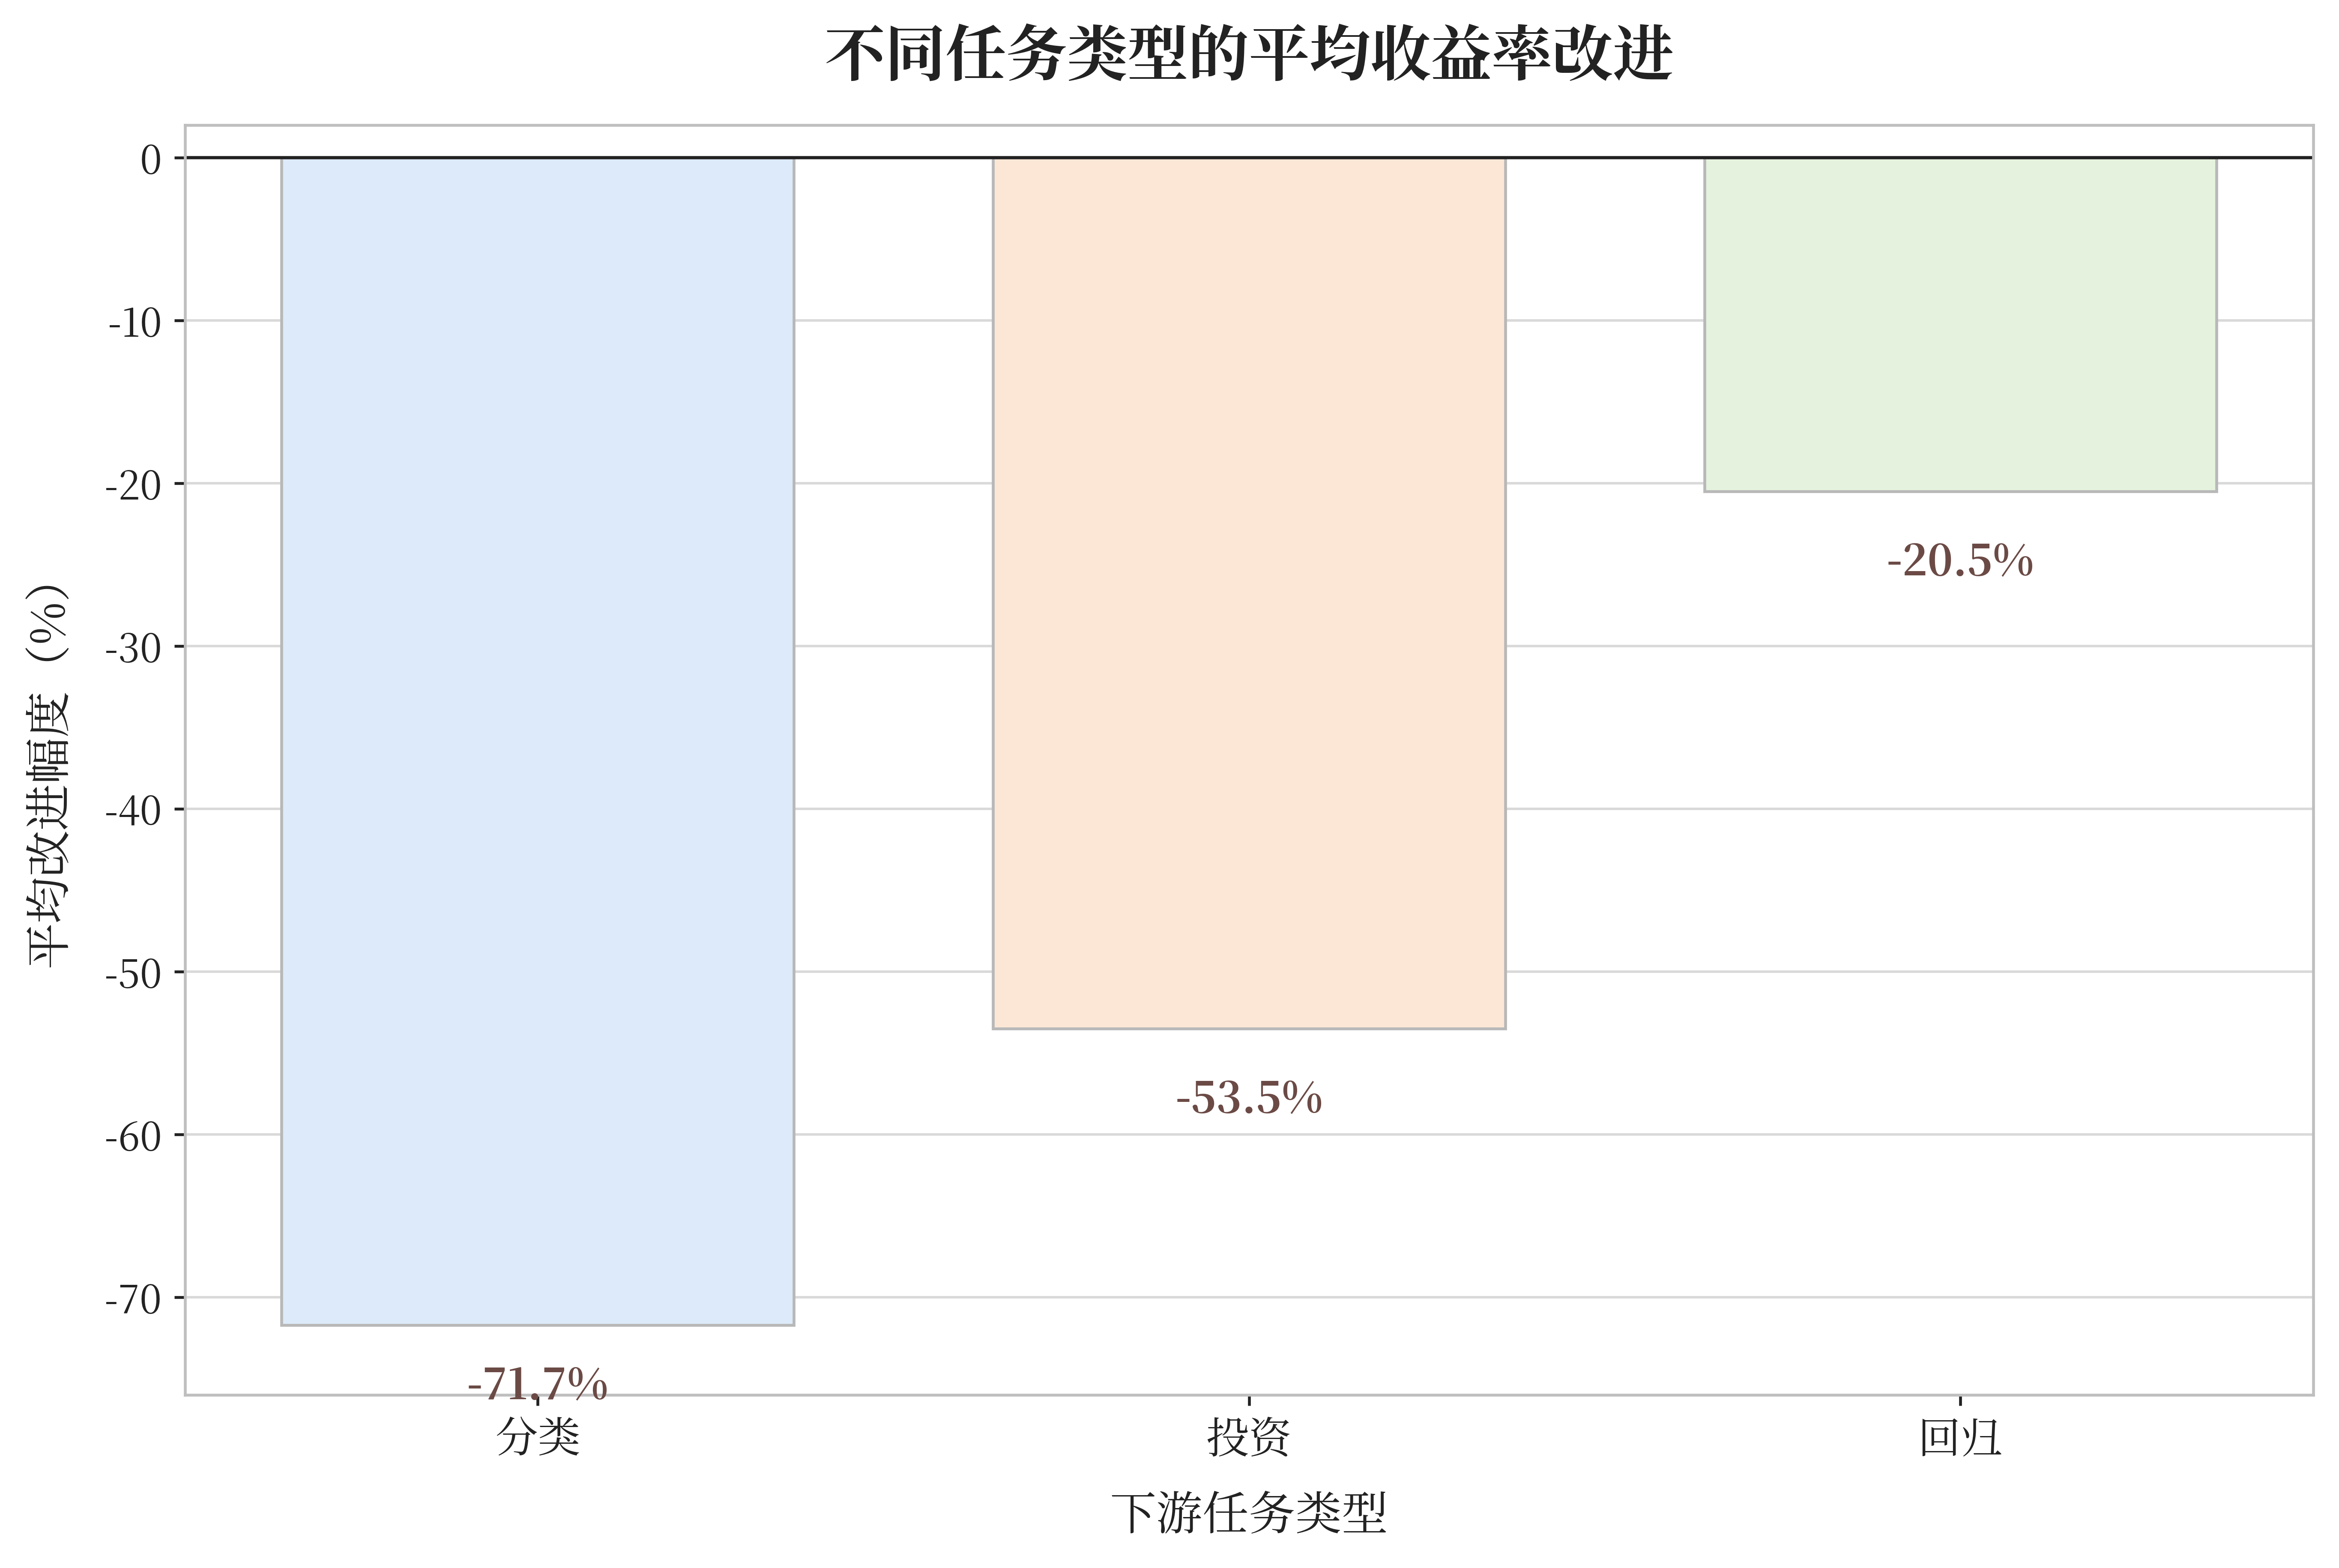
\includegraphics[width=0.8\textwidth]{figures/chap4/fig4_task_comparison_cn.png} 
    \caption{不同任务类型的平均收益改进幅度}
    \label{fig:highdimtaskcomp}
\end{figure}

三类任务中，回归任务的平均收益改进更为明显，棉花（+340\%）、动力煤（+195.51\%）、白糖（+36.40\%）均属增幅较大的案例。回归任务要求输出连续价格值，不同生成器在预测精度上的差异在连续空间中更容易被动态评估机制捕捉。动力煤是“亏损转盈利”的典型案例：基准模型回测亏损-16.23\%，赛马场竞争机制将其转为+15.50\%盈利。图\ref{fig:highdimcoalpredcom}先从价格预测层面对比两类模型的拟合效果，用于观察动态竞争是否改善了局部价格波动的跟踪能力。

% \begin{figure}[h!]
%     \centering 
%     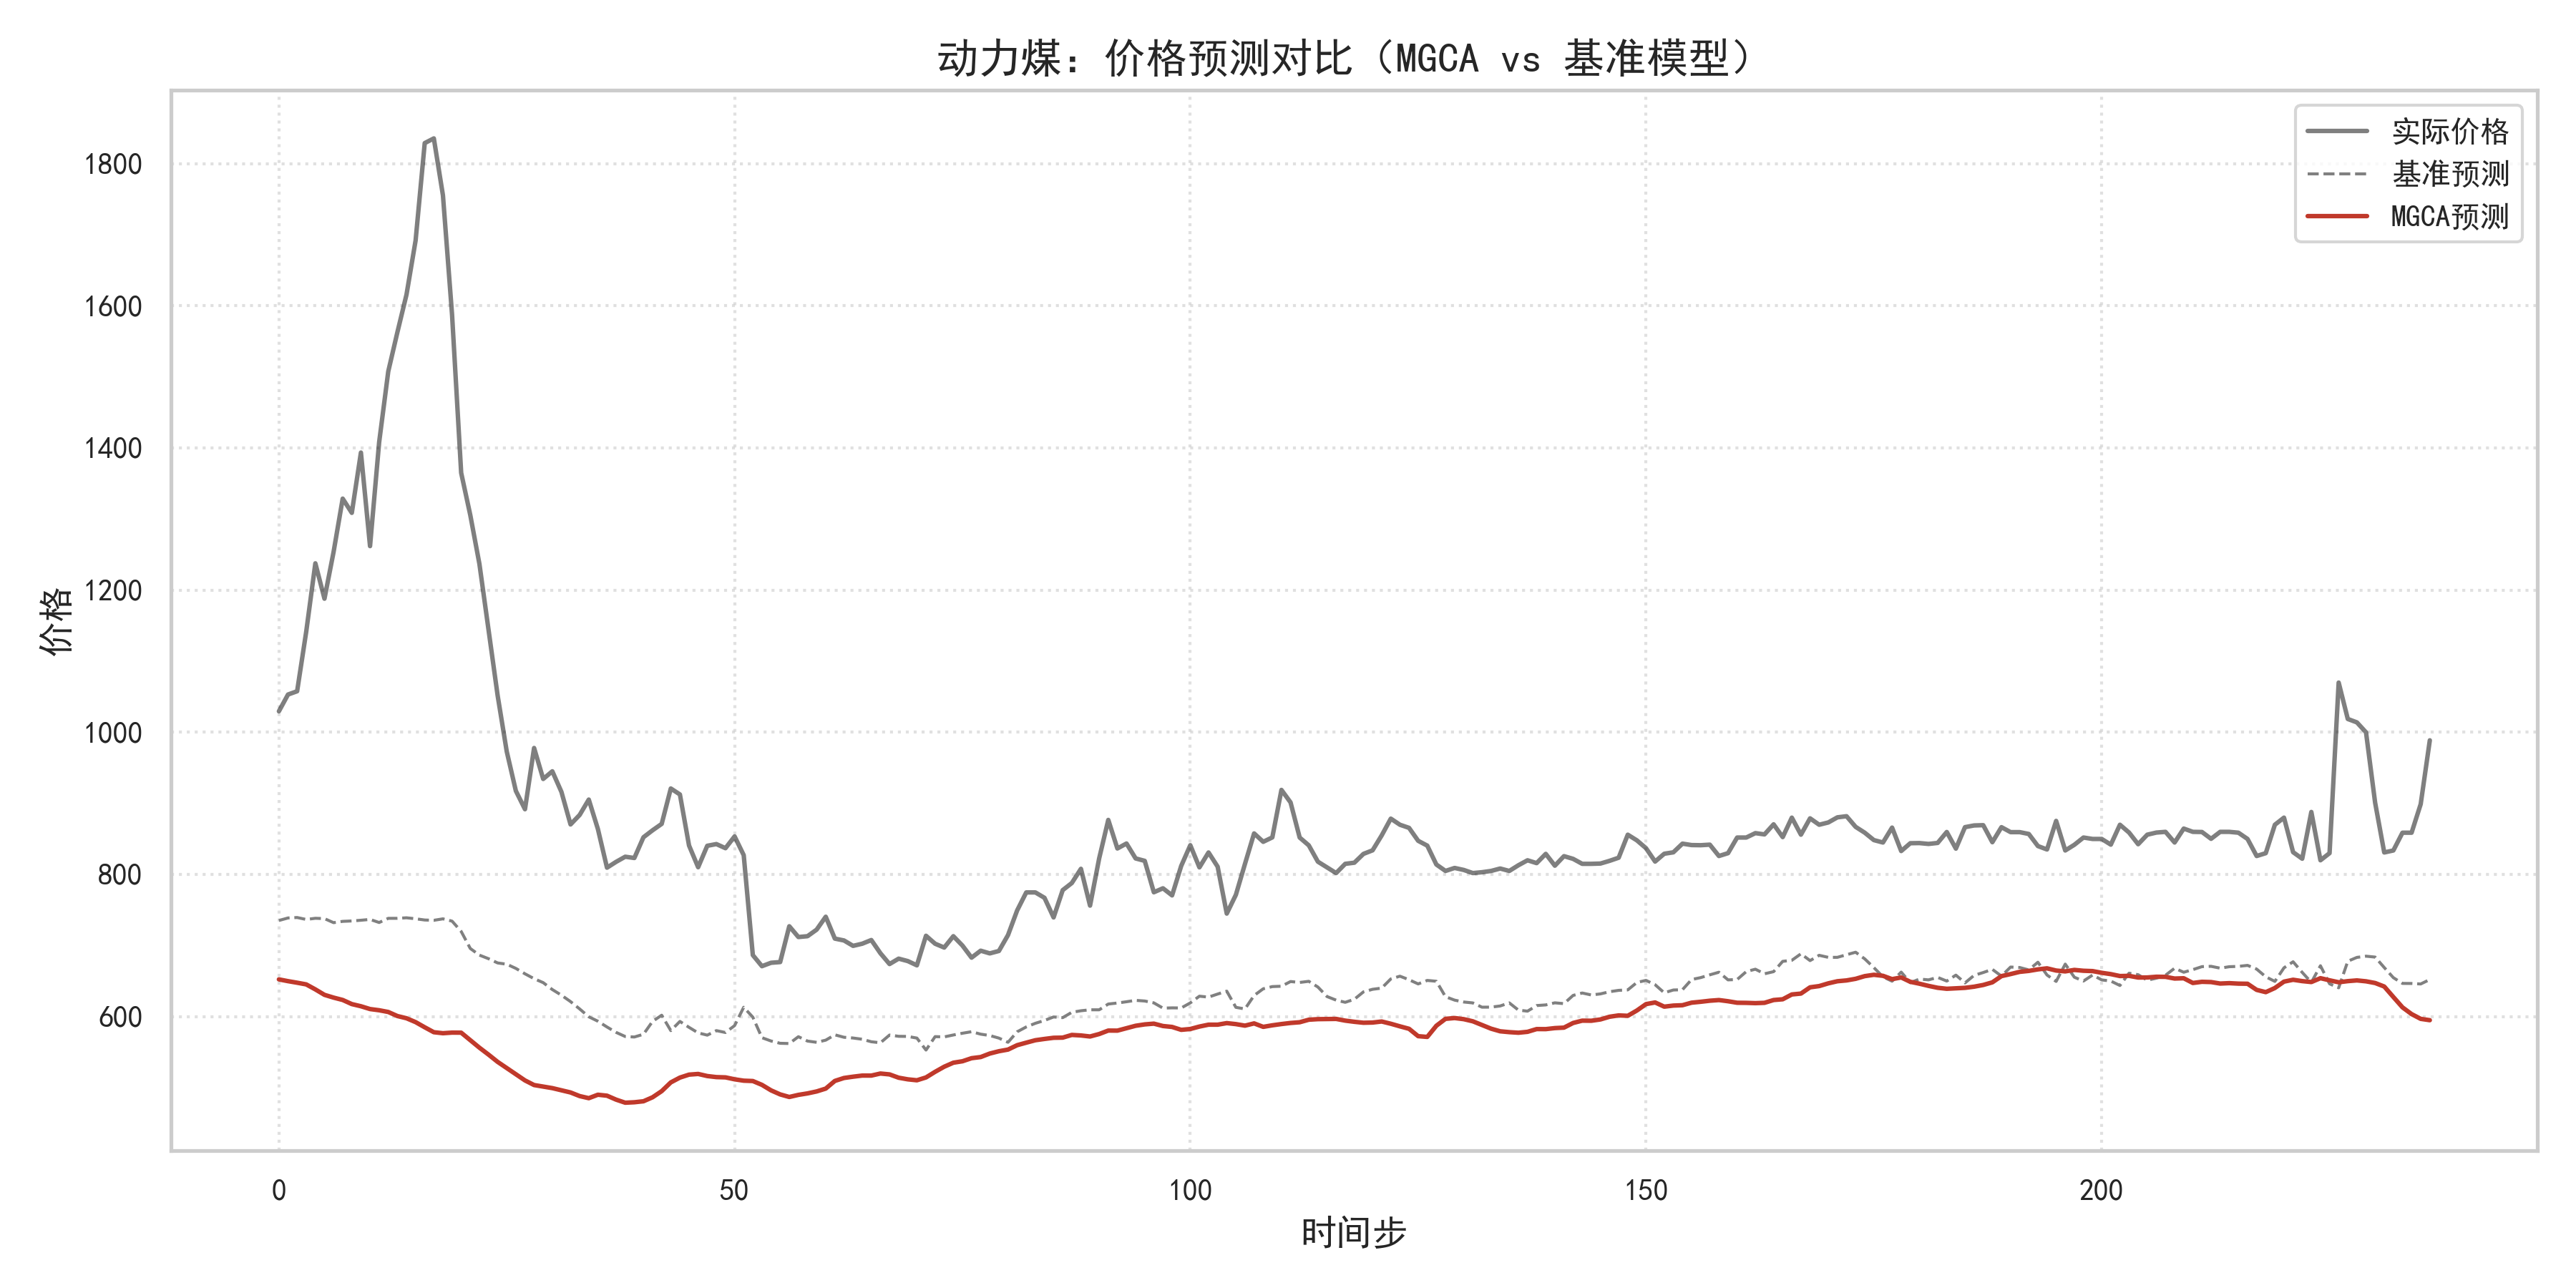
\includegraphics[width=0.8\textwidth]{figures/chap4/fig9_coal_pred_comparison_cn.png} 
%     \caption{动力煤价格逐日预测拟合对比}
%     \label{fig:highdimcoalpredcom}
% \end{figure}
\begin{figure}[!htbp]
    \centering 
    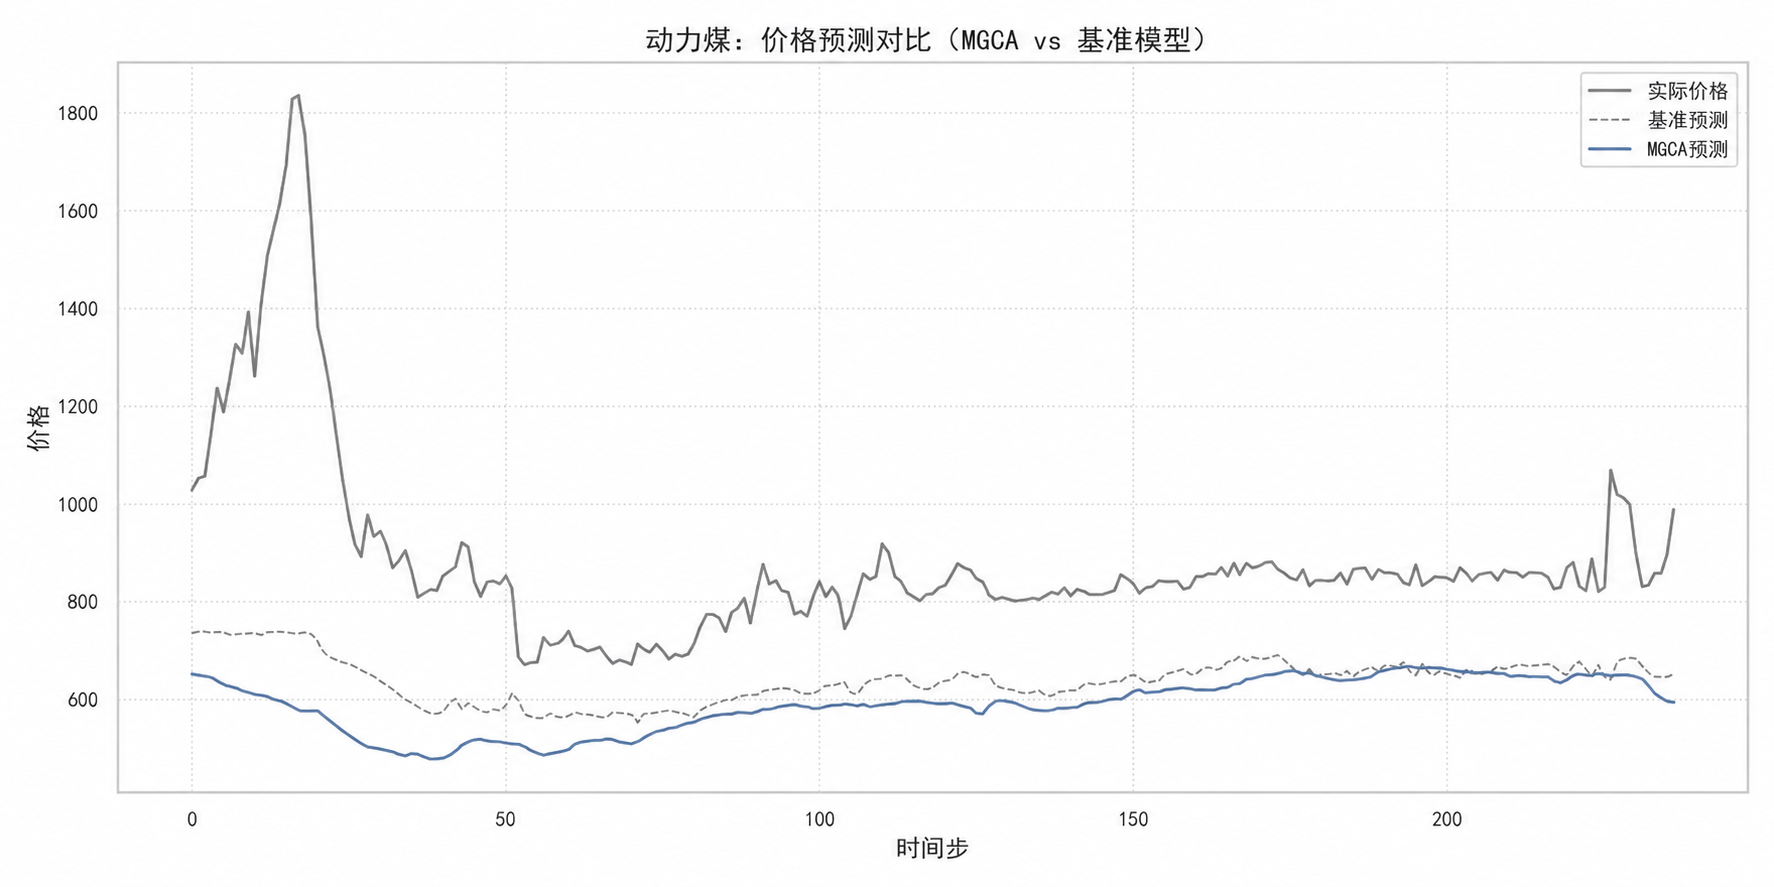
\includegraphics[width=0.8\textwidth]{figures/chap4/图3.8改.png} 
    \caption{动力煤价格逐日预测拟合对比}
    \label{fig:highdimcoalpredcom}
\end{figure}

若价格拟合改善能够转化为交易收益，则累计收益曲线应呈现更稳定的净值修复过程。图\ref{fig:highdimcoalequitycurve}进一步给出动力煤真实回测累计收益曲线，用于检验预测改善是否落实到回测收益层面。



% \begin{figure}[h!]
%     \centering 
%     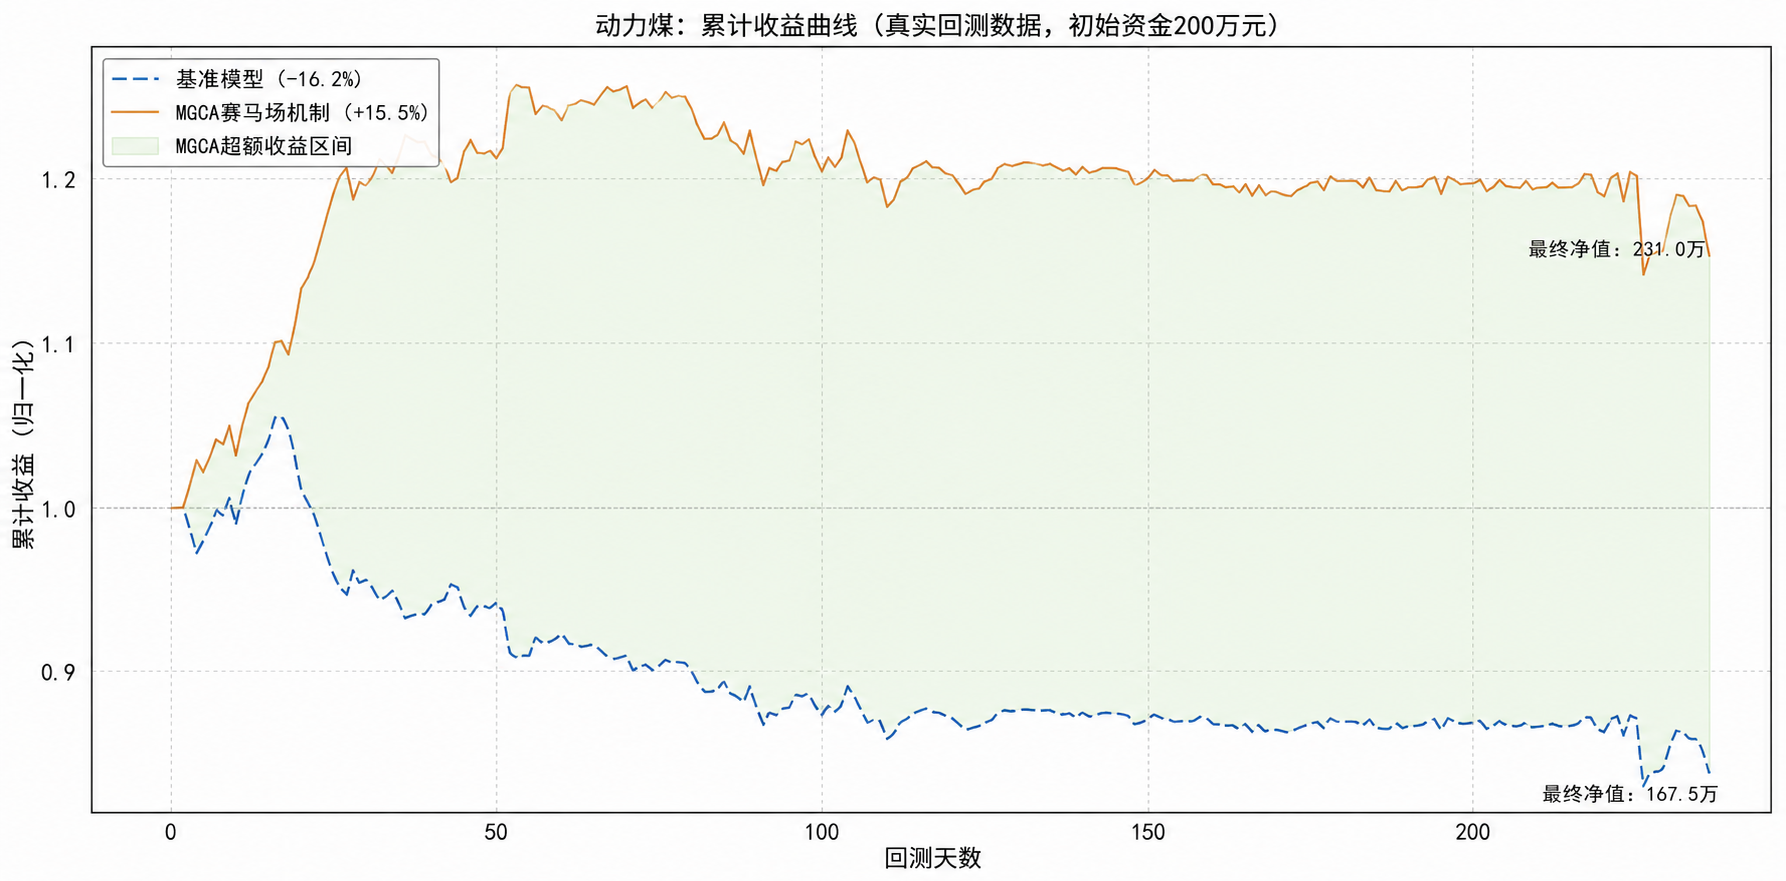
\includegraphics[width=0.8\textwidth]{figures/chap4/fig9_coal_equity_curve_cn.png} 
%     \caption{动力煤真实回测累计收益曲线（初始资金200万元）}
%     \label{fig:highdimcoalequitycurve}
% \end{figure}

\begin{figure}[!htbp]
    \centering 
    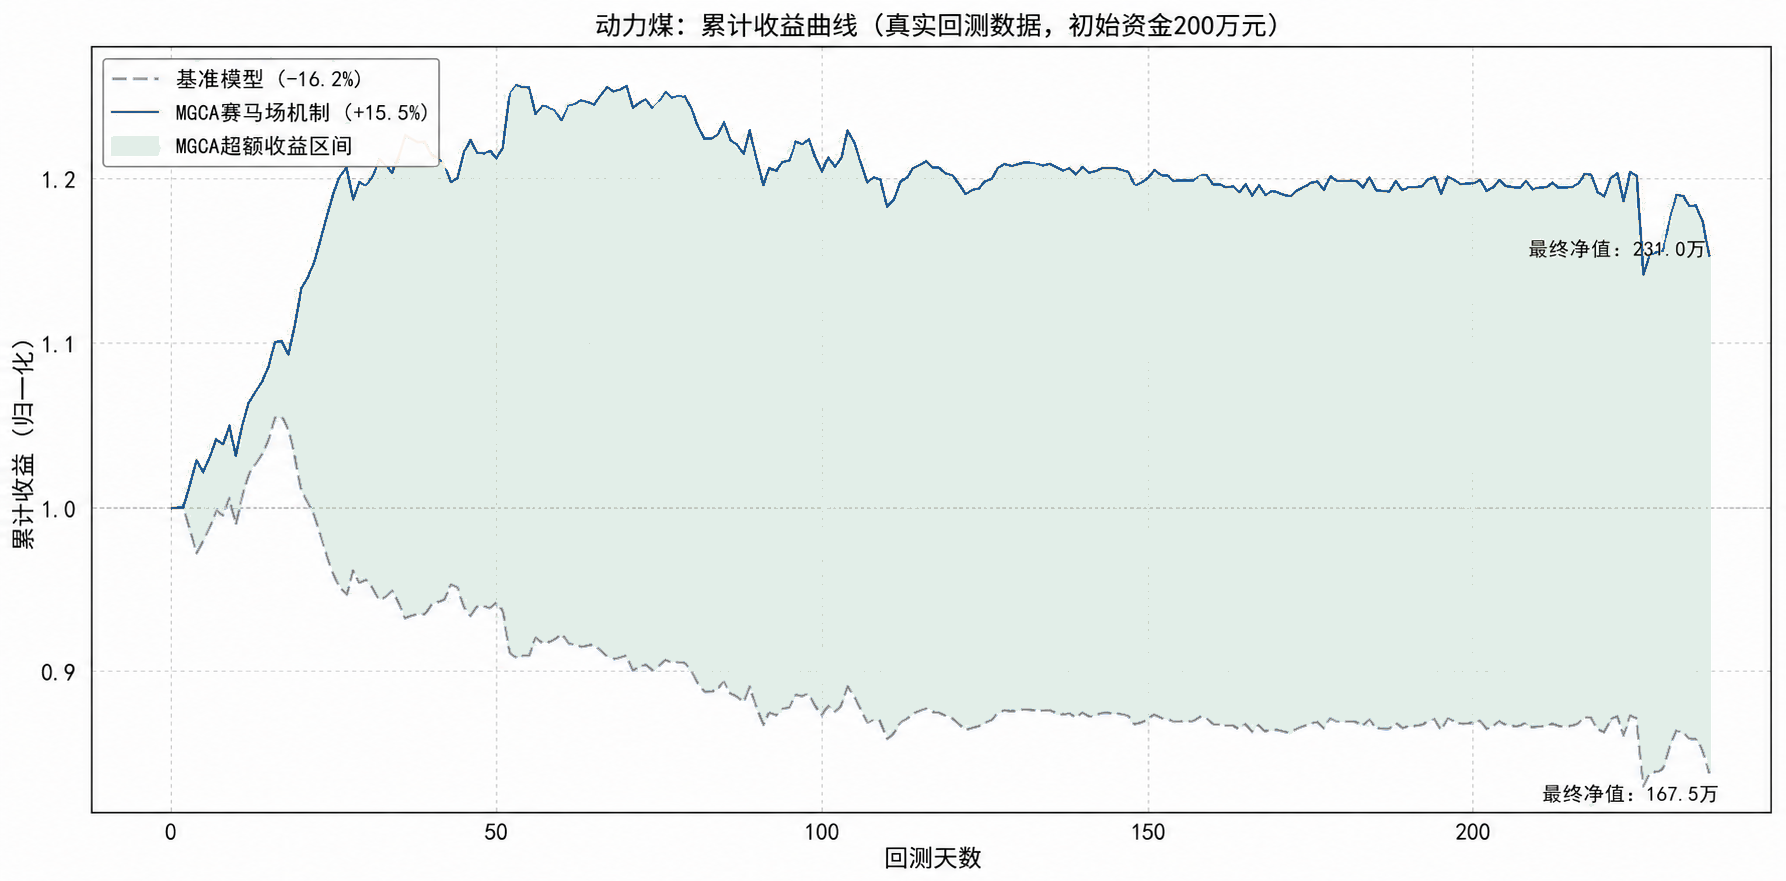
\includegraphics[width=0.8\textwidth]{figures/chap4/图3.9改.png} 
    \caption{动力煤真实回测累计收益曲线（初始资金200万元）}
    \label{fig:highdimcoalequitycurve}
\end{figure}

从动力煤案例看，赛马场竞争机制的作用不只是降低点预测误差，更重要的是在趋势变化阶段减少错误方向累积，使价格预测改善能够转化为收益曲线修复。
棉花（Cotton）是本章中改进幅度最大的单品案例。先从预测拟合层面看，图~\ref{fig:highdimcottonpredcomp}展示了棉花价格逐日预测拟合对比，赛马场竞争机制在价格急剧变化区间的预测误差低于基准模型。该图主要说明动态竞争机制能够在局部波动较强的区间中选择更适合当前状态的生成器输出。

% \begin{figure}[h!]
%     \centering 
%     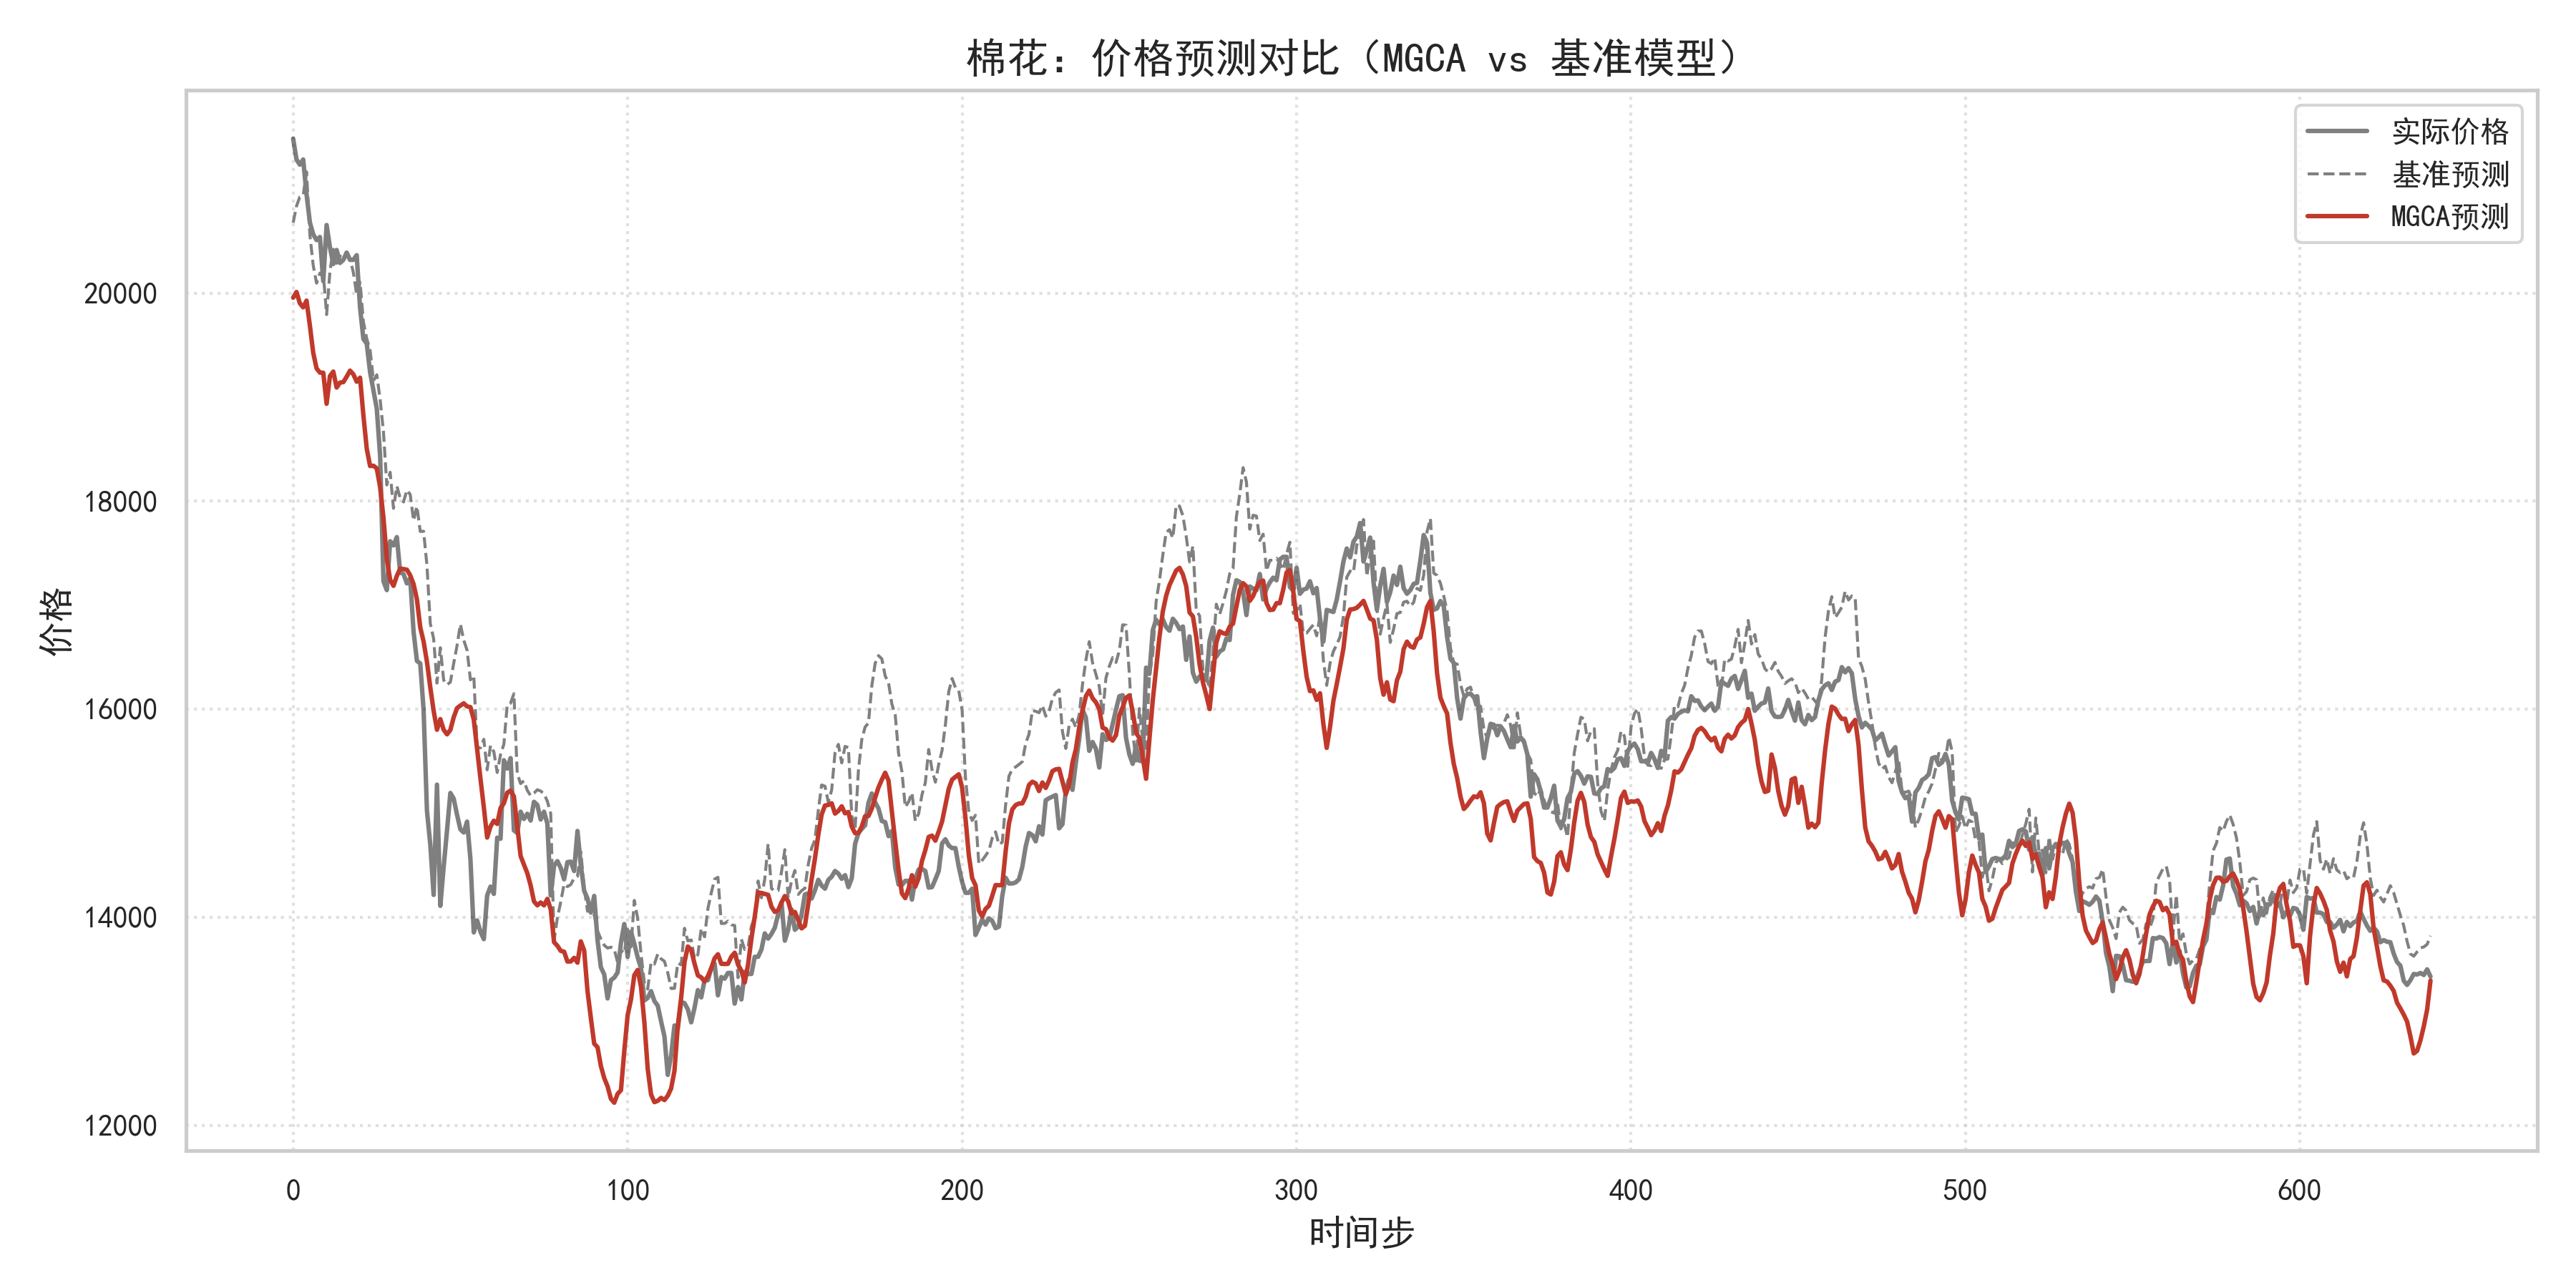
\includegraphics[width=0.8\textwidth]{figures/chap4/fig8_cotton_pred_comparison_cn.png} 
%     \caption{棉花价格逐日预测拟合对比}
%     \label{fig:highdimcottonpredcomp}
% \end{figure}

\begin{figure}[!htbp]
    \centering 
    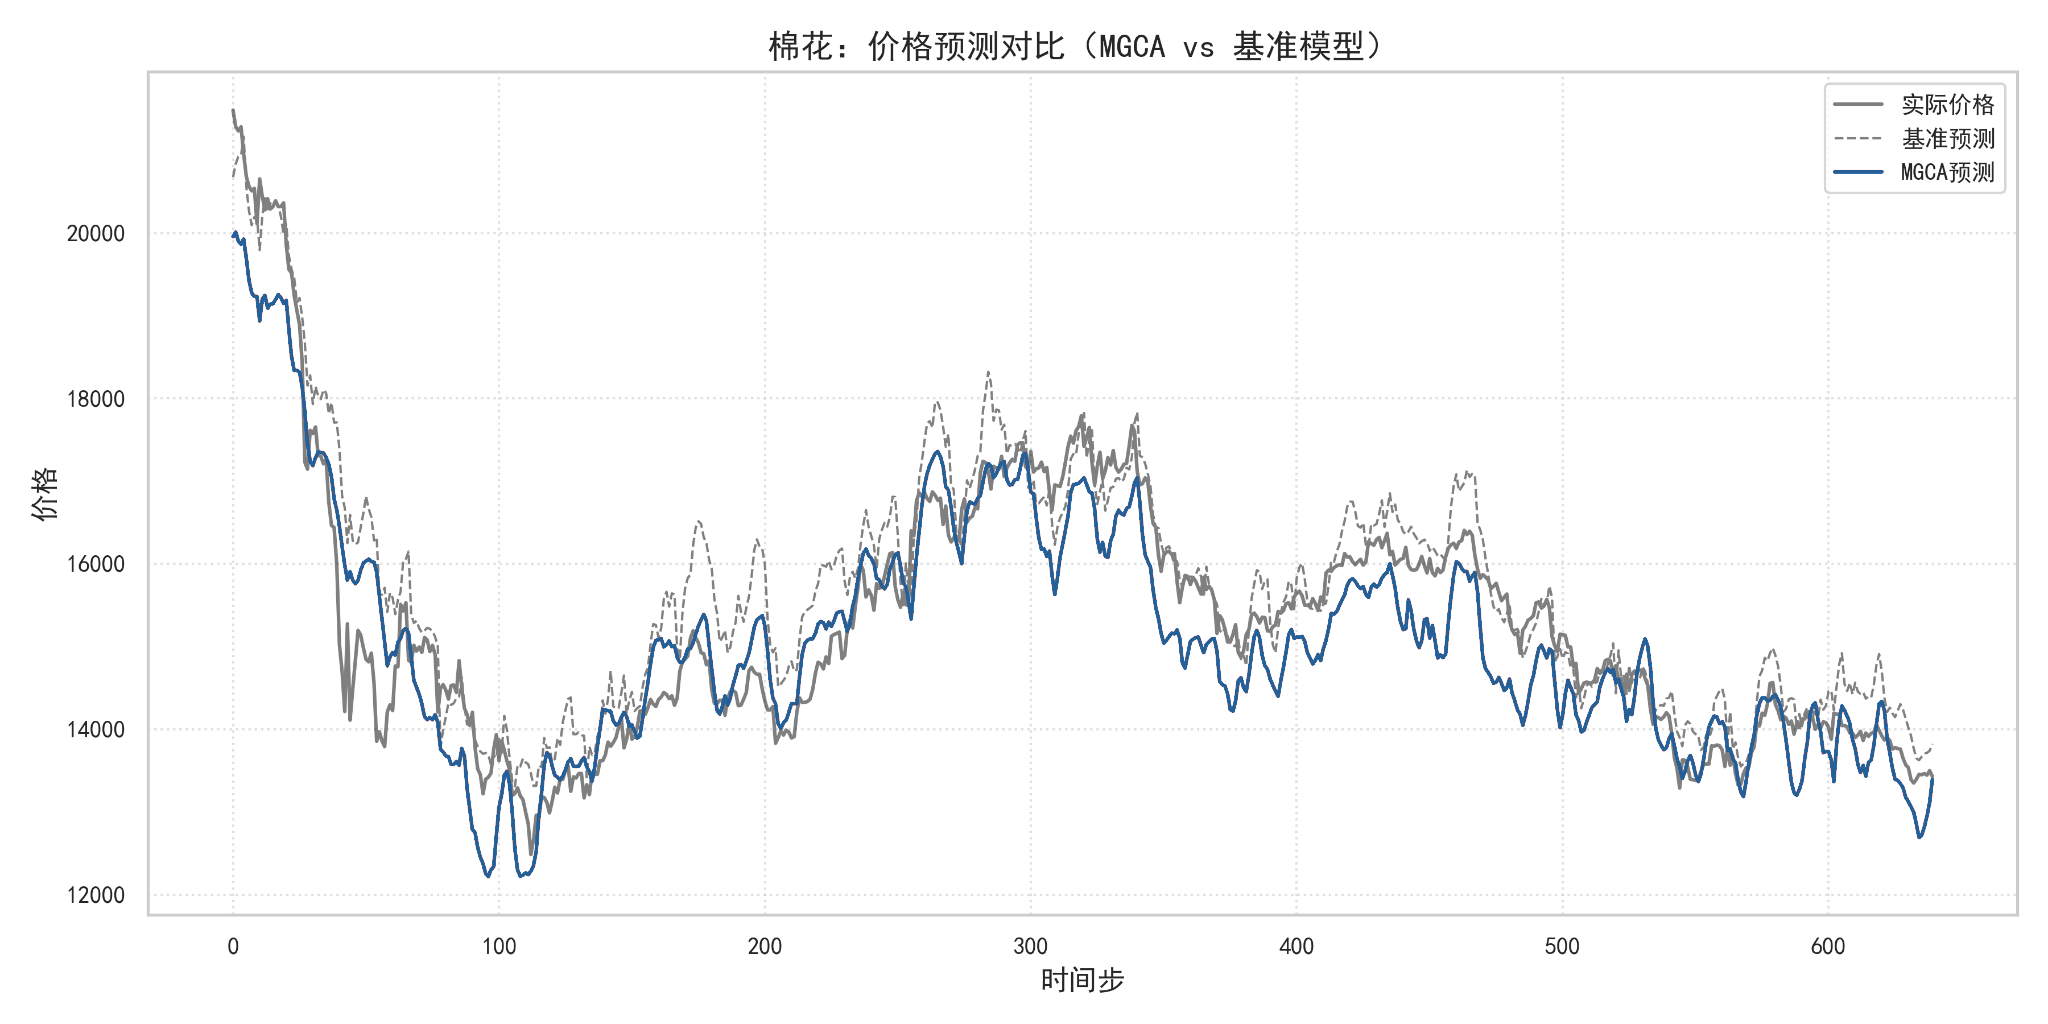
\includegraphics[width=0.8\textwidth]{figures/chap4/图3.10改.png} 
    \caption{棉花价格逐日预测拟合对比}
    \label{fig:highdimcottonpredcomp}
\end{figure}

进一步看，预测拟合优势是否具有交易意义，需要结合真实回测收益曲线进行判断。图~\ref{fig:highdimcottonequitycurve}呈现了棉花真实回测累计收益曲线，赛马场竞争机制最终收益+165.5\%（净值531万），高于基准模型的+37.6\%（净值275万）。


% \begin{figure}[h!]
%     \centering 
%     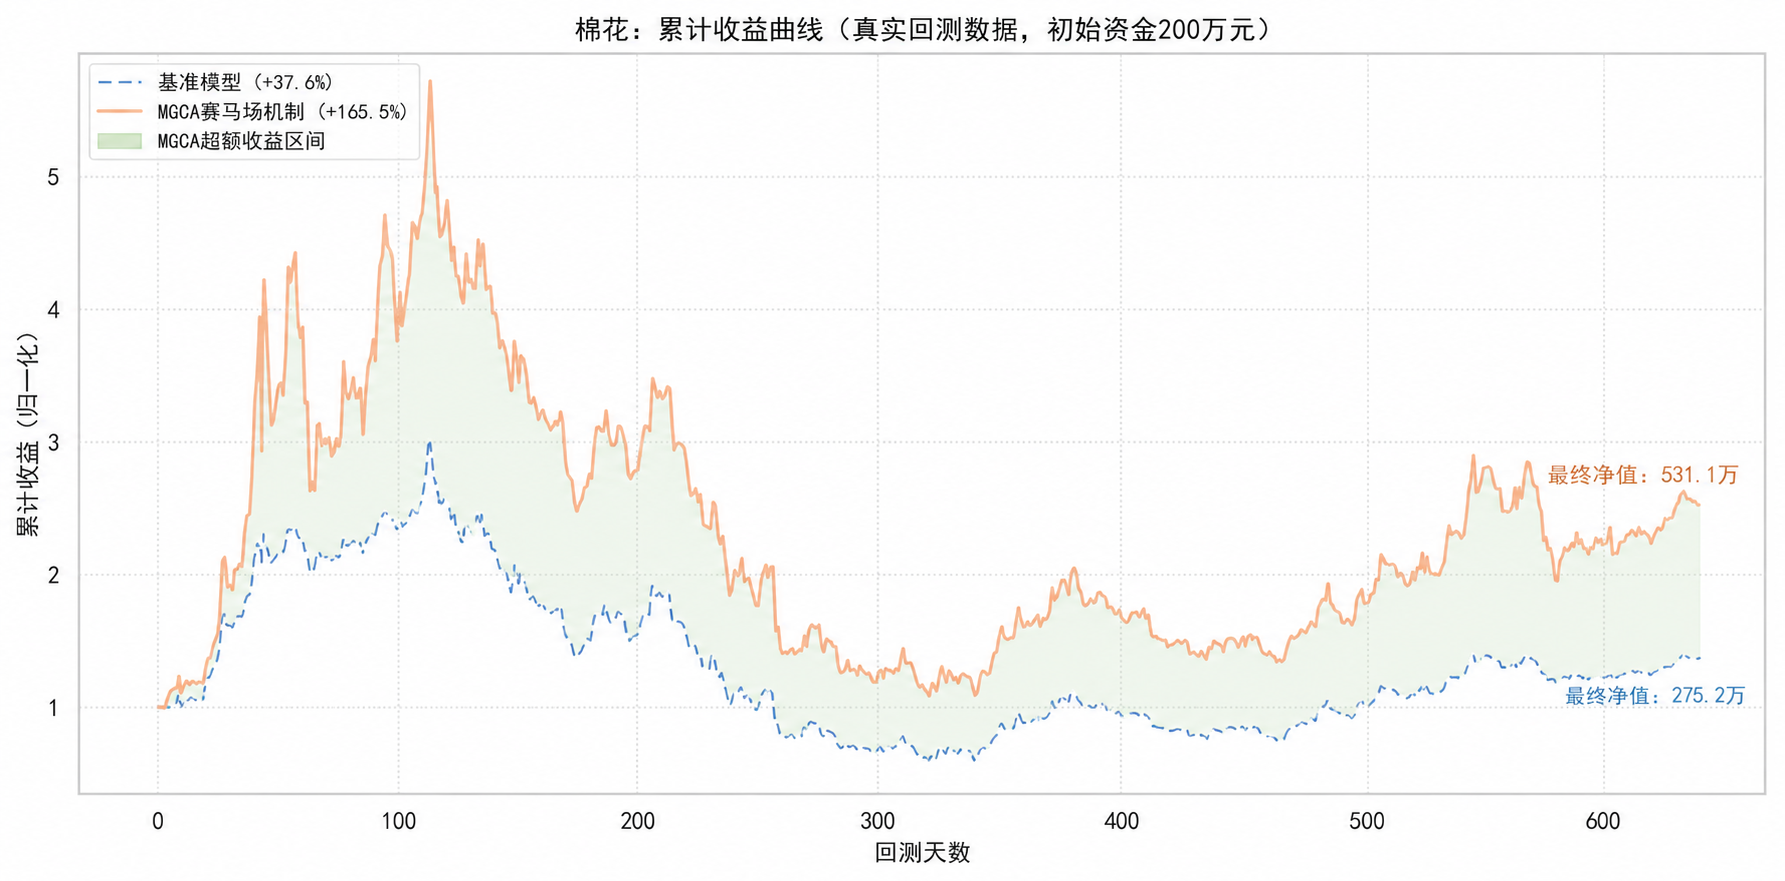
\includegraphics[width=0.8\textwidth]{figures/chap4/fig8_cotton_equity_curve_cn.png} 
%     \caption{棉花真实回测累计收益曲线}
%     \label{fig:highdimcottonequitycurve}
% \end{figure}
\begin{figure}[!htbp]
    \centering 
    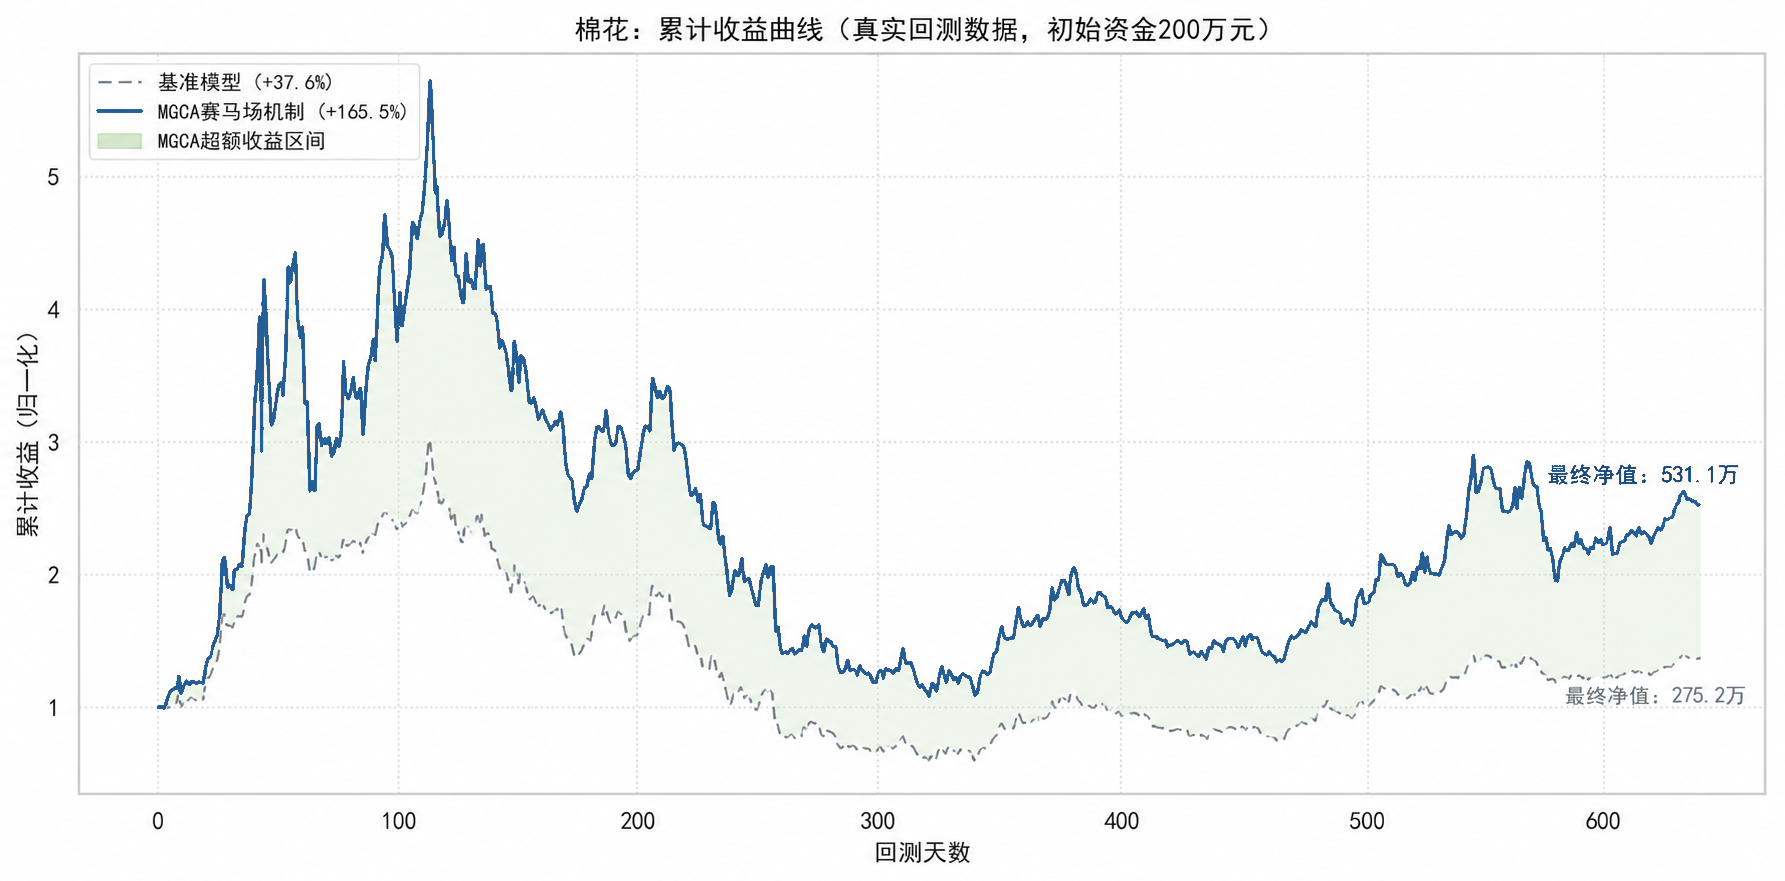
\includegraphics[width=0.8\textwidth]{figures/chap4/图3.11改.png} 
    \caption{棉花真实回测累计收益曲线}
    \label{fig:highdimcottonequitycurve}
\end{figure}

表~\ref{tab:cottoPerformance}进一步列出棉花回归任务的详细性能对比。该表用于补充说明收益提升并非只体现在曲线形态上，也反映在最终净值和收益率等量化指标中；同时，最大回撤略有增加，提示该案例的收益改善仍伴随一定风险代价。


\begin{table}[!htbp]
\centering
\caption{棉花（Cotton）回归任务详细性能对比}
\label{tab:cottoPerformance}
\small
\setlength{\tabcolsep}{4pt}
\renewcommand{\arraystretch}{1.15}
\begin{tabular}{>{\raggedright\arraybackslash}p{3.8cm} >{\centering\arraybackslash}p{2.6cm} >{\centering\arraybackslash}p{3.2cm} >{\centering\arraybackslash}p{2.2cm}}
\toprule
\textbf{指标} & \textbf{基准模型} & \textbf{赛马场竞争机制} & \textbf{变化} \\
\midrule
策略收益率 (Return \%) & 37.58\% & \textbf{165.33\%} & \textbf{+340.00\%} \\
最终净值 (Final Value) & ¥2,751,503 & \textbf{¥5,306,581} & \textbf{+92.86\%} \\
最大回撤 (Max Drawdown) & 80.34\% & 81.02\% & +0.85\% \\
初始资本 (Initial Capital) & ¥2,000,000 & ¥2,000,000 & -- \\
回测交易日 (Trading Days) & 639 & 639 & -- \\
\bottomrule
\end{tabular}
\end{table}

为解释棉花案例中的收益改善来源，后续图表进一步观察模型群体内部的动态选择过程。图~\ref{fig:highdimcottonradar}从多生成器排名热力图角度展示不同生成器在训练与评估过程中的相对位置变化。


% \begin{figure}[h!]
%     \centering 
%     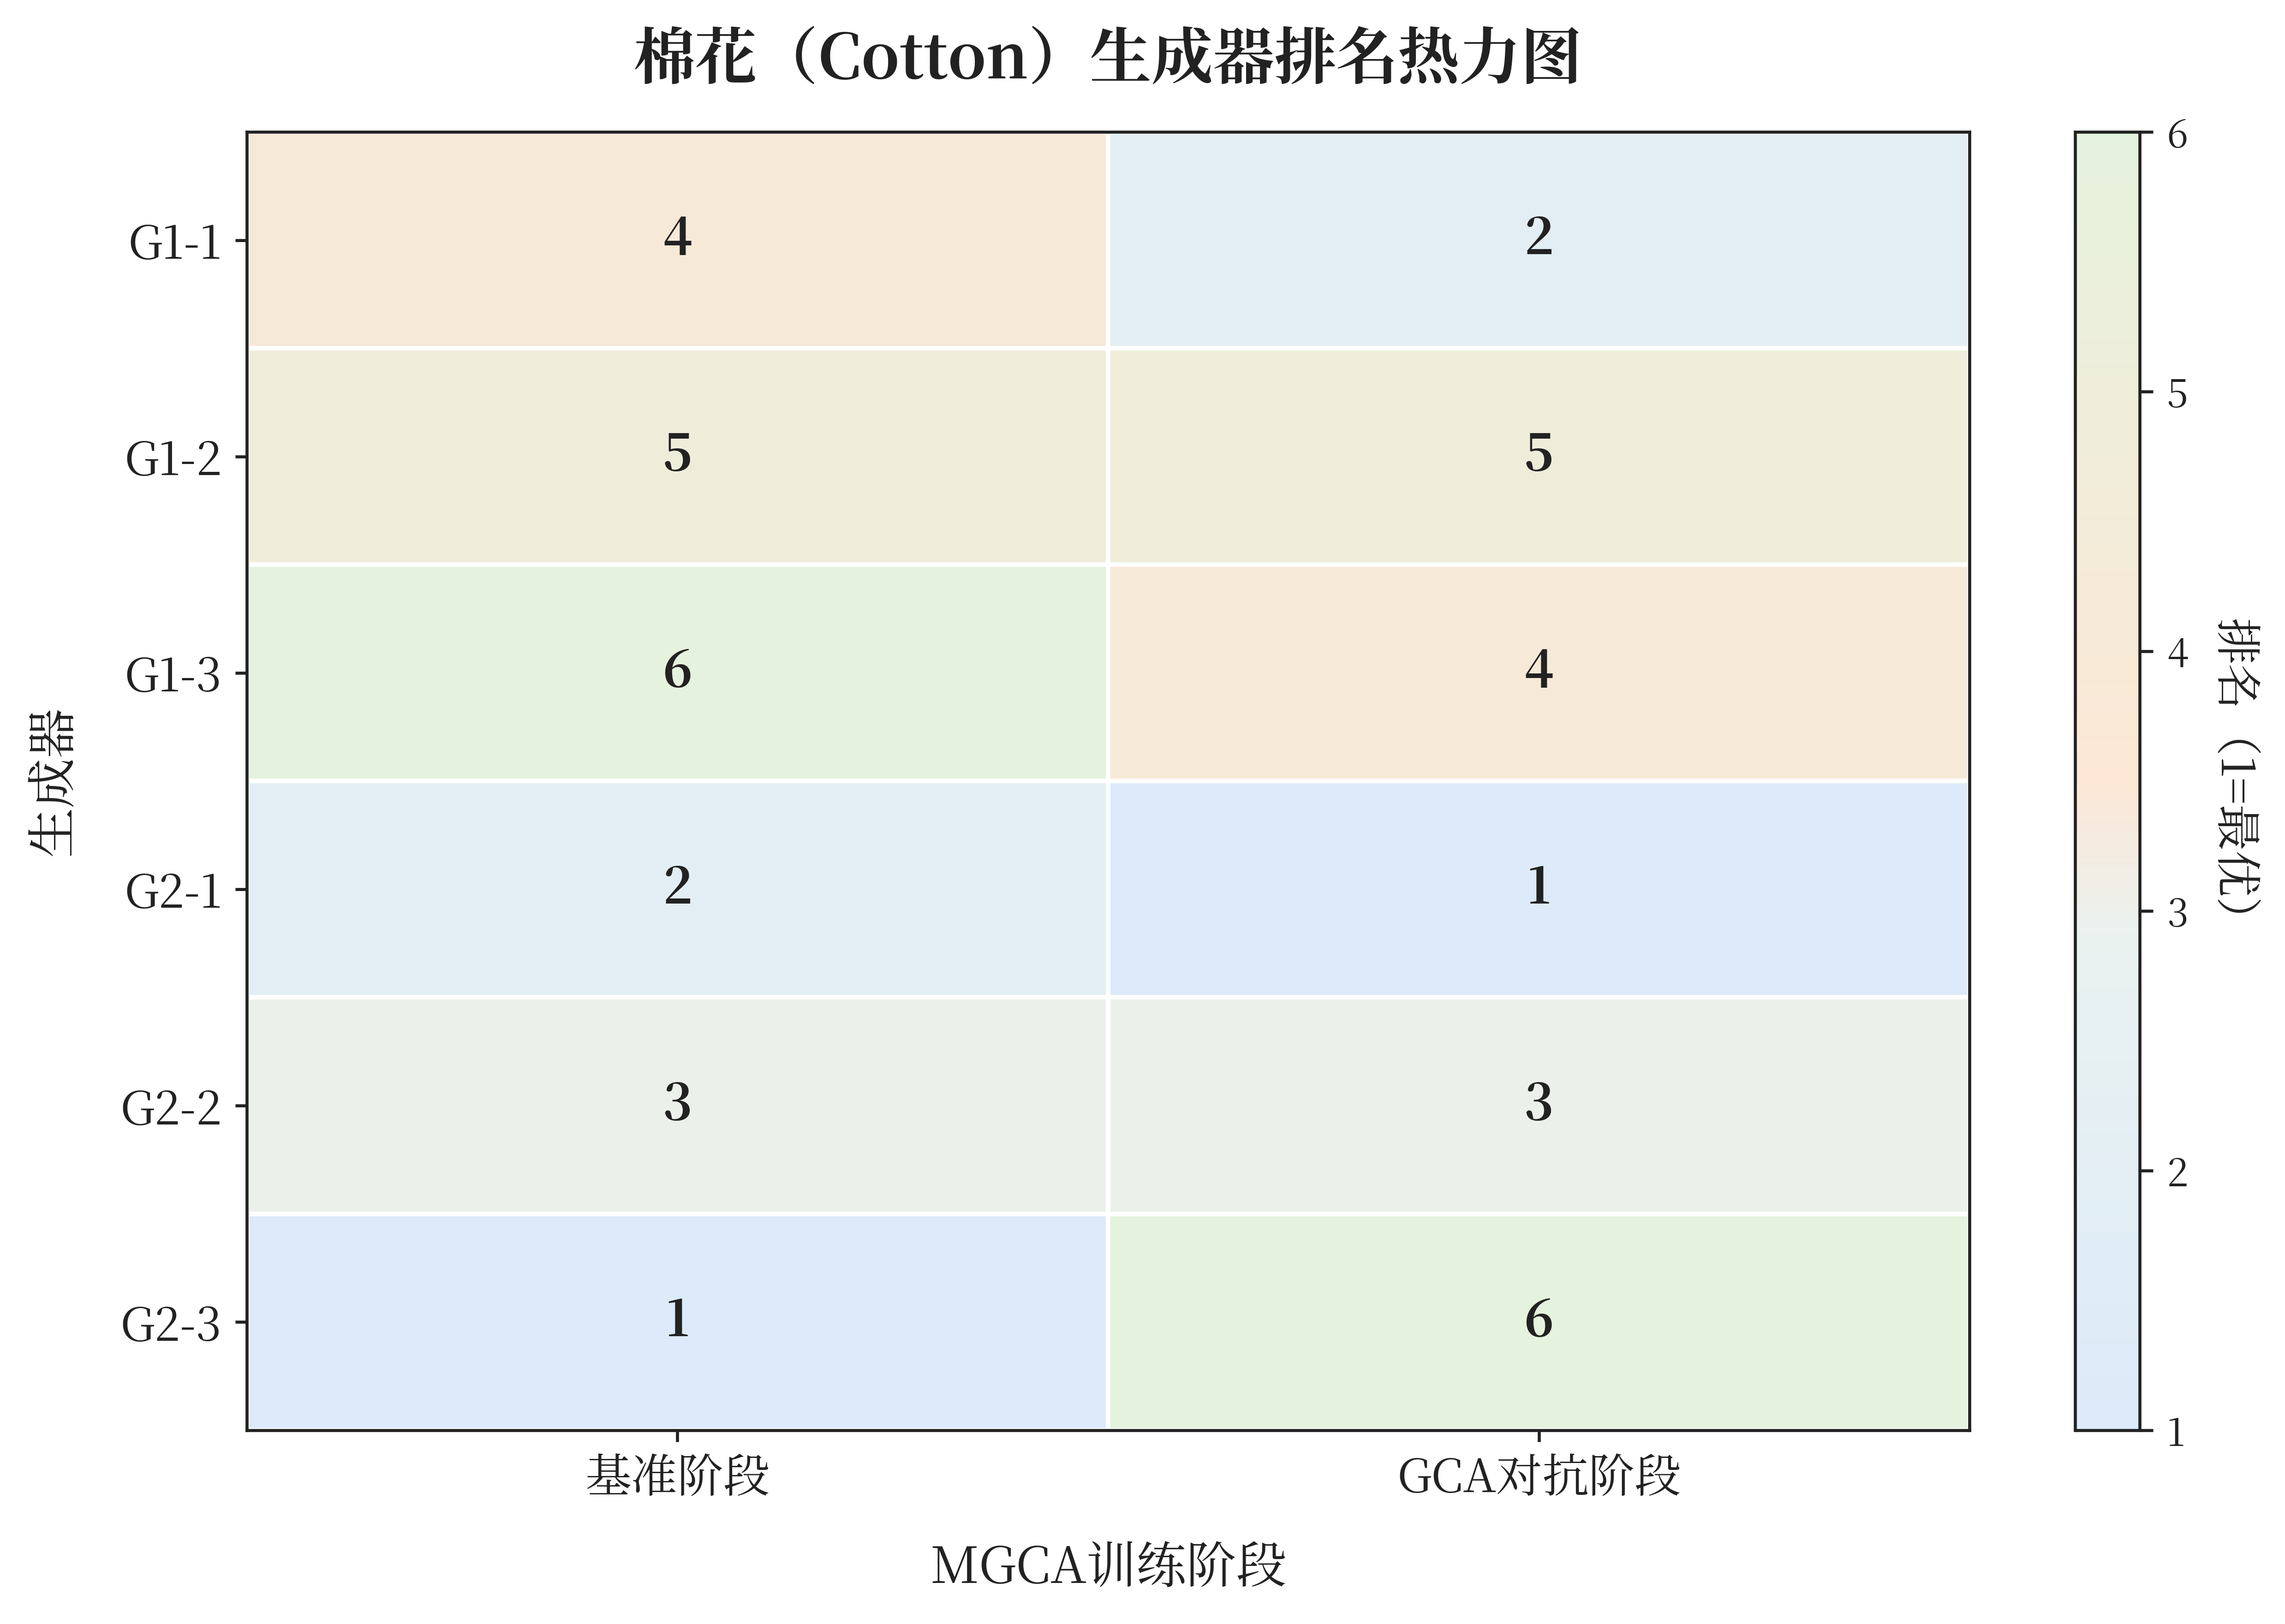
\includegraphics[width=0.8\textwidth]{figures/chap4/fig_cotton_ranking_heatmap_cn.png} 
%     \caption{棉花回归任务多生成器排名热力图}
%     \label{fig:highdimcottonradar}
% \end{figure}

\begin{figure}[!htbp]
    \centering 
    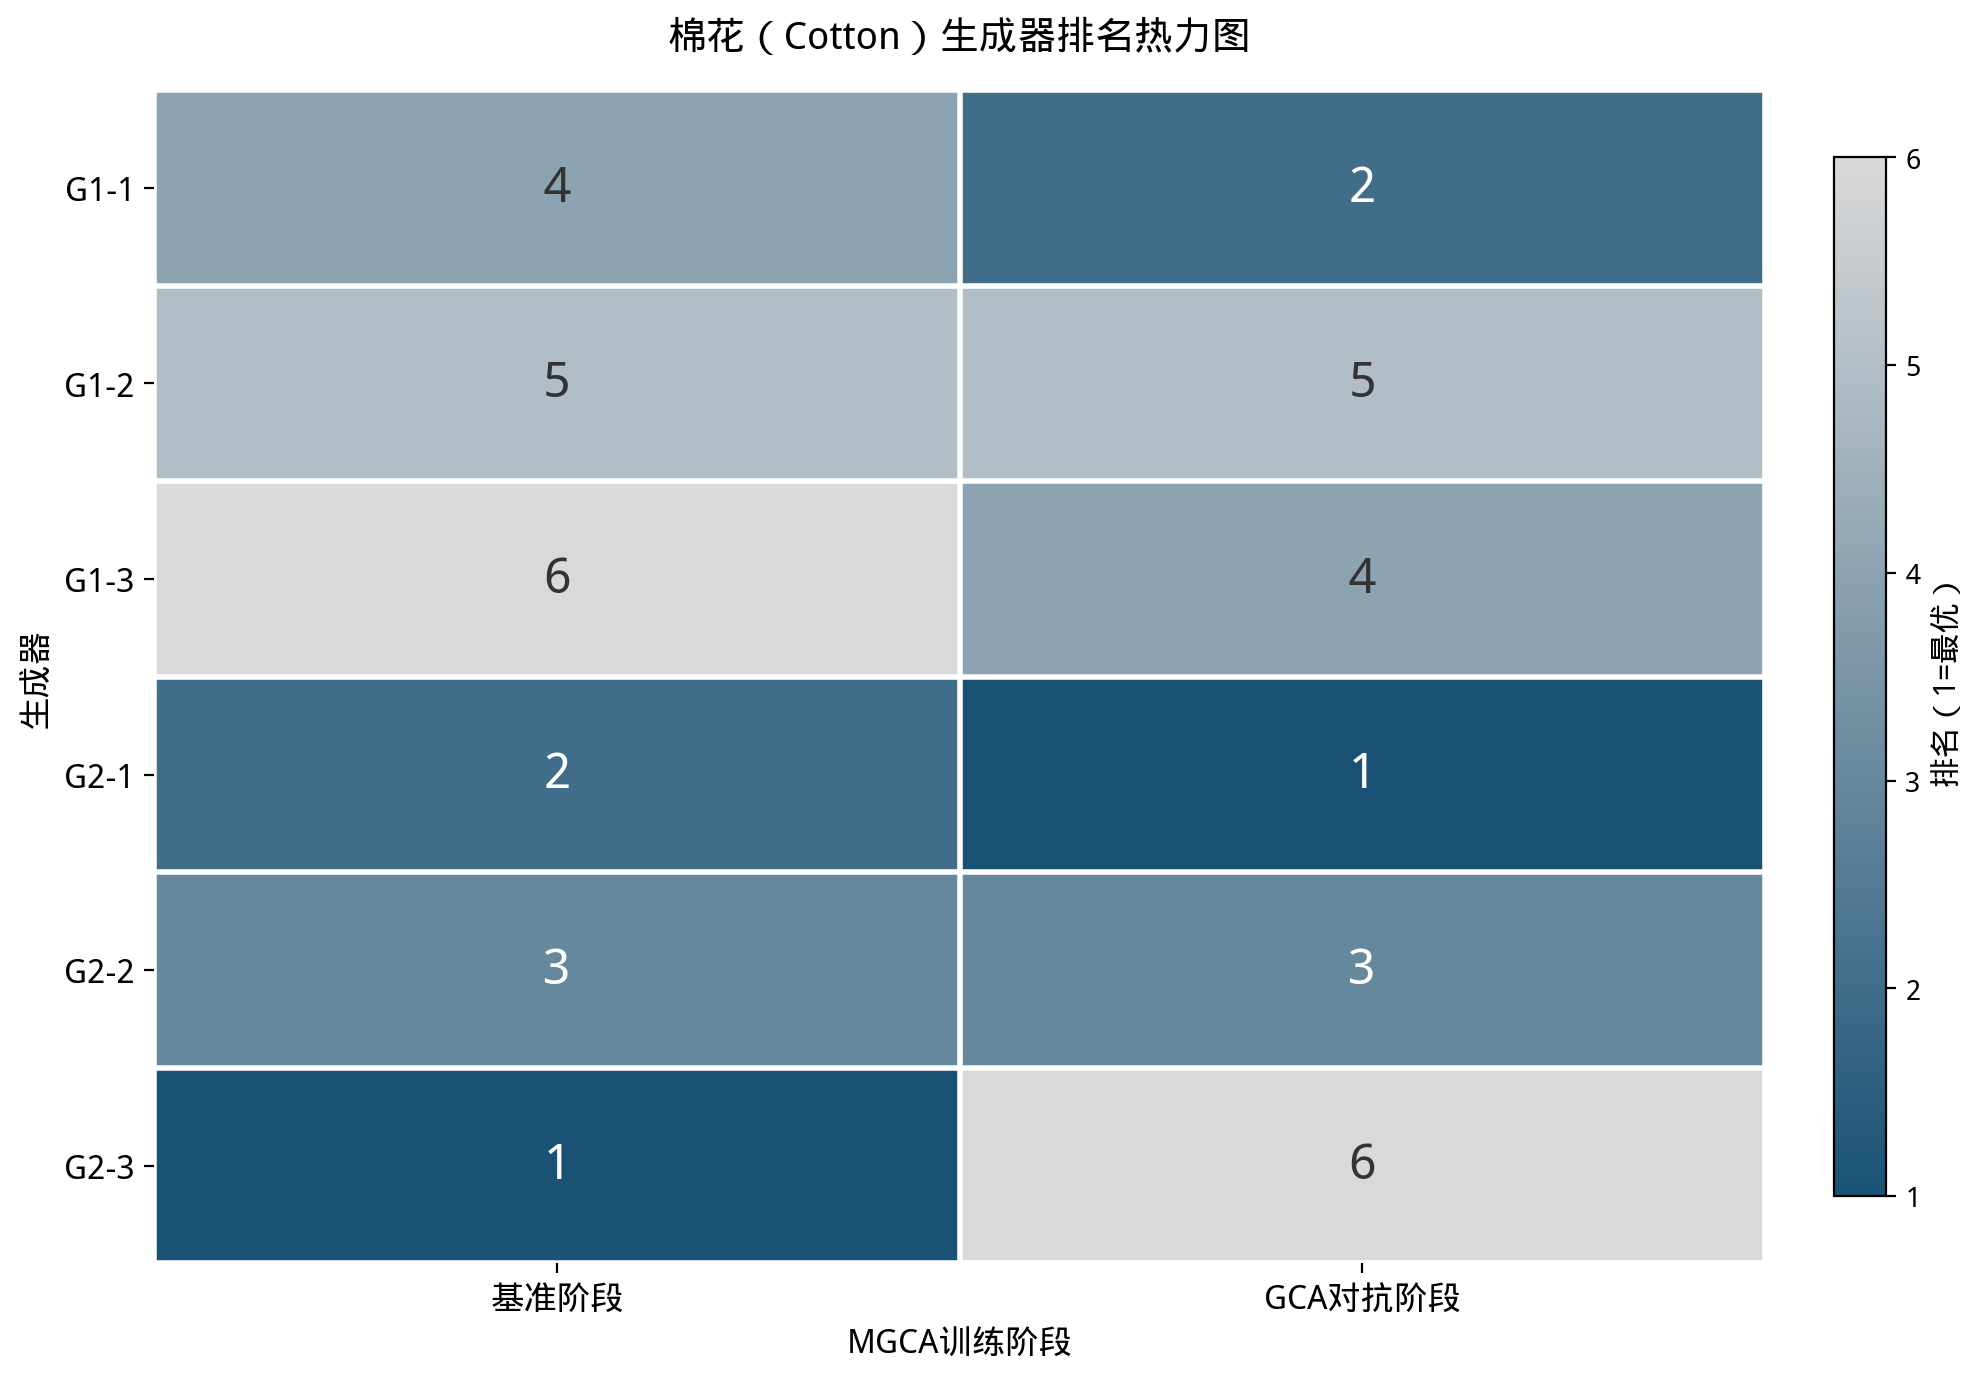
\includegraphics[width=0.8\textwidth]{figures/chap4/图3.12改.png} 
    \caption{棉花回归任务多生成器排名热力图}
    \label{fig:highdimcottonradar}
\end{figure}

图~\ref{fig:highdimcottonhm}则从多维性能雷达图角度补充观察棉花案例中的收益、回撤和风险调整表现。两张图共同说明，棉花案例的改进不是单一模型偶然胜出，而是动态选择机制在不同生成器之间持续比较后的结果。


\begin{figure}[!htbp]
    \centering 
    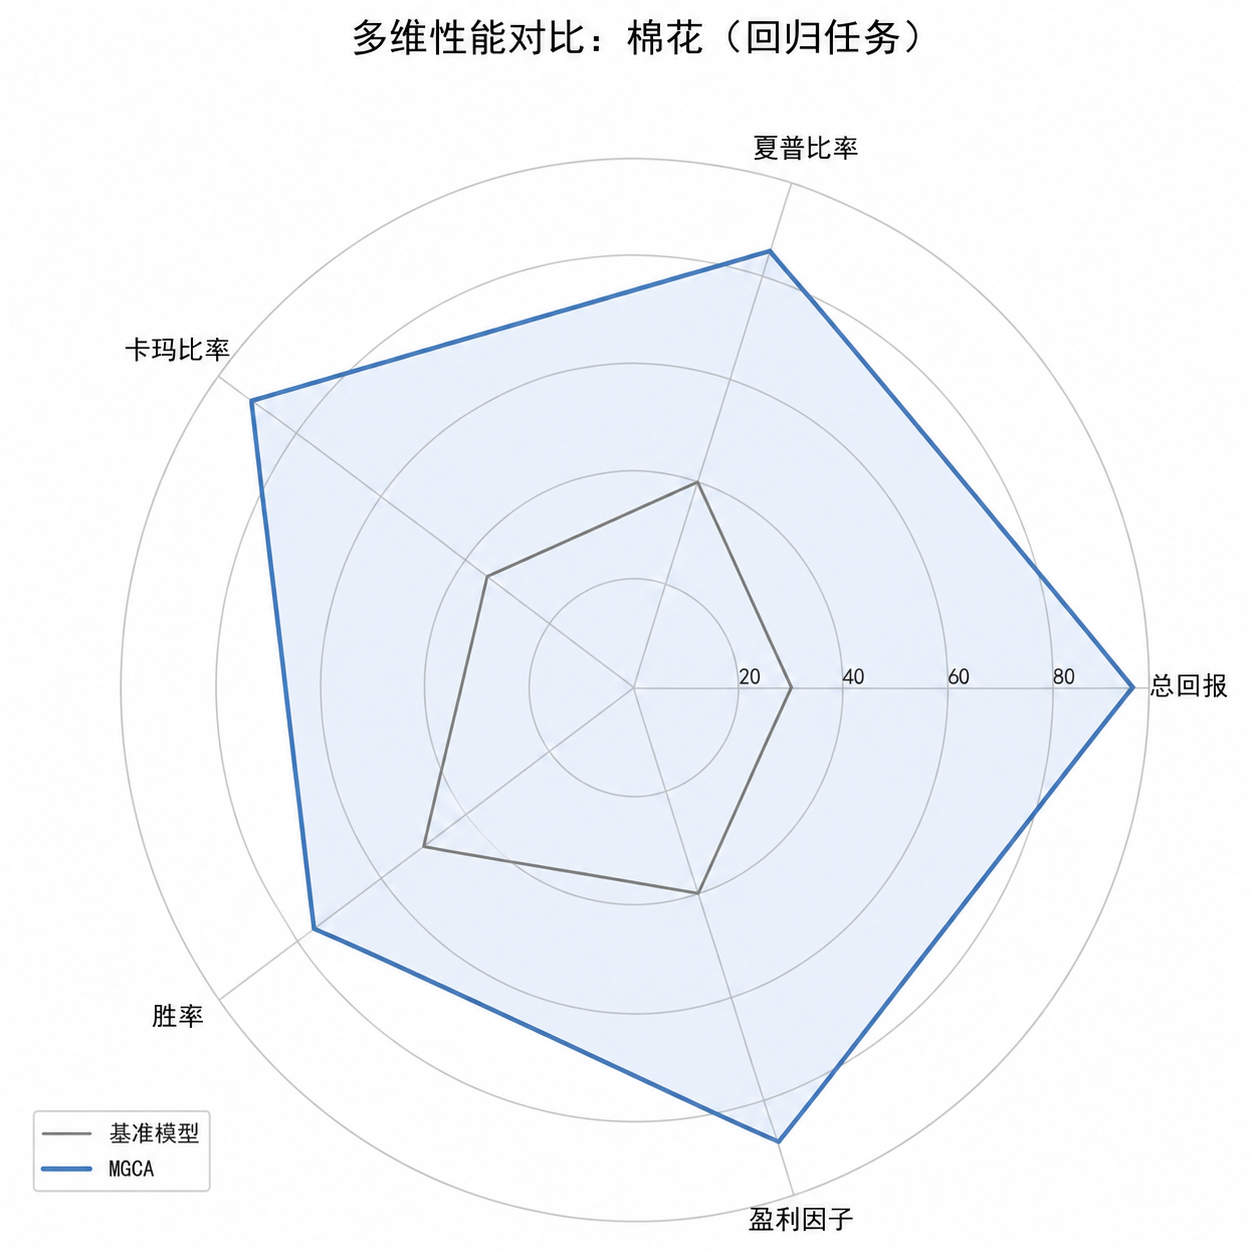
\includegraphics[width=0.8\textwidth]{figures/chap4/fig6_radar_cotton_cn.png}
    \caption{棉花回归任务多维性能雷达图}
    \label{fig:highdimcottonhm}
\end{figure}

在典型案例分析之后，进一步需要考察赛马场竞争机制是否改变了模型学习过程本身。图\ref{fig:highdimtrainingmsecomp}展示了All-Assets组中16种资产在回归任务下赛马场竞争机制与基准模型的训练均方误差对比，以均方误差比率（赛马场竞争机制/基准模型）的形式呈现，小于1.0表示赛马场竞争机制的训练误差更低。该图的目的不是证明所有资产的训练误差都降低，而是观察动态竞争机制是否在不同品种上形成差异化学习效果。

% \begin{figure}[htbp]
%     \centering 
%     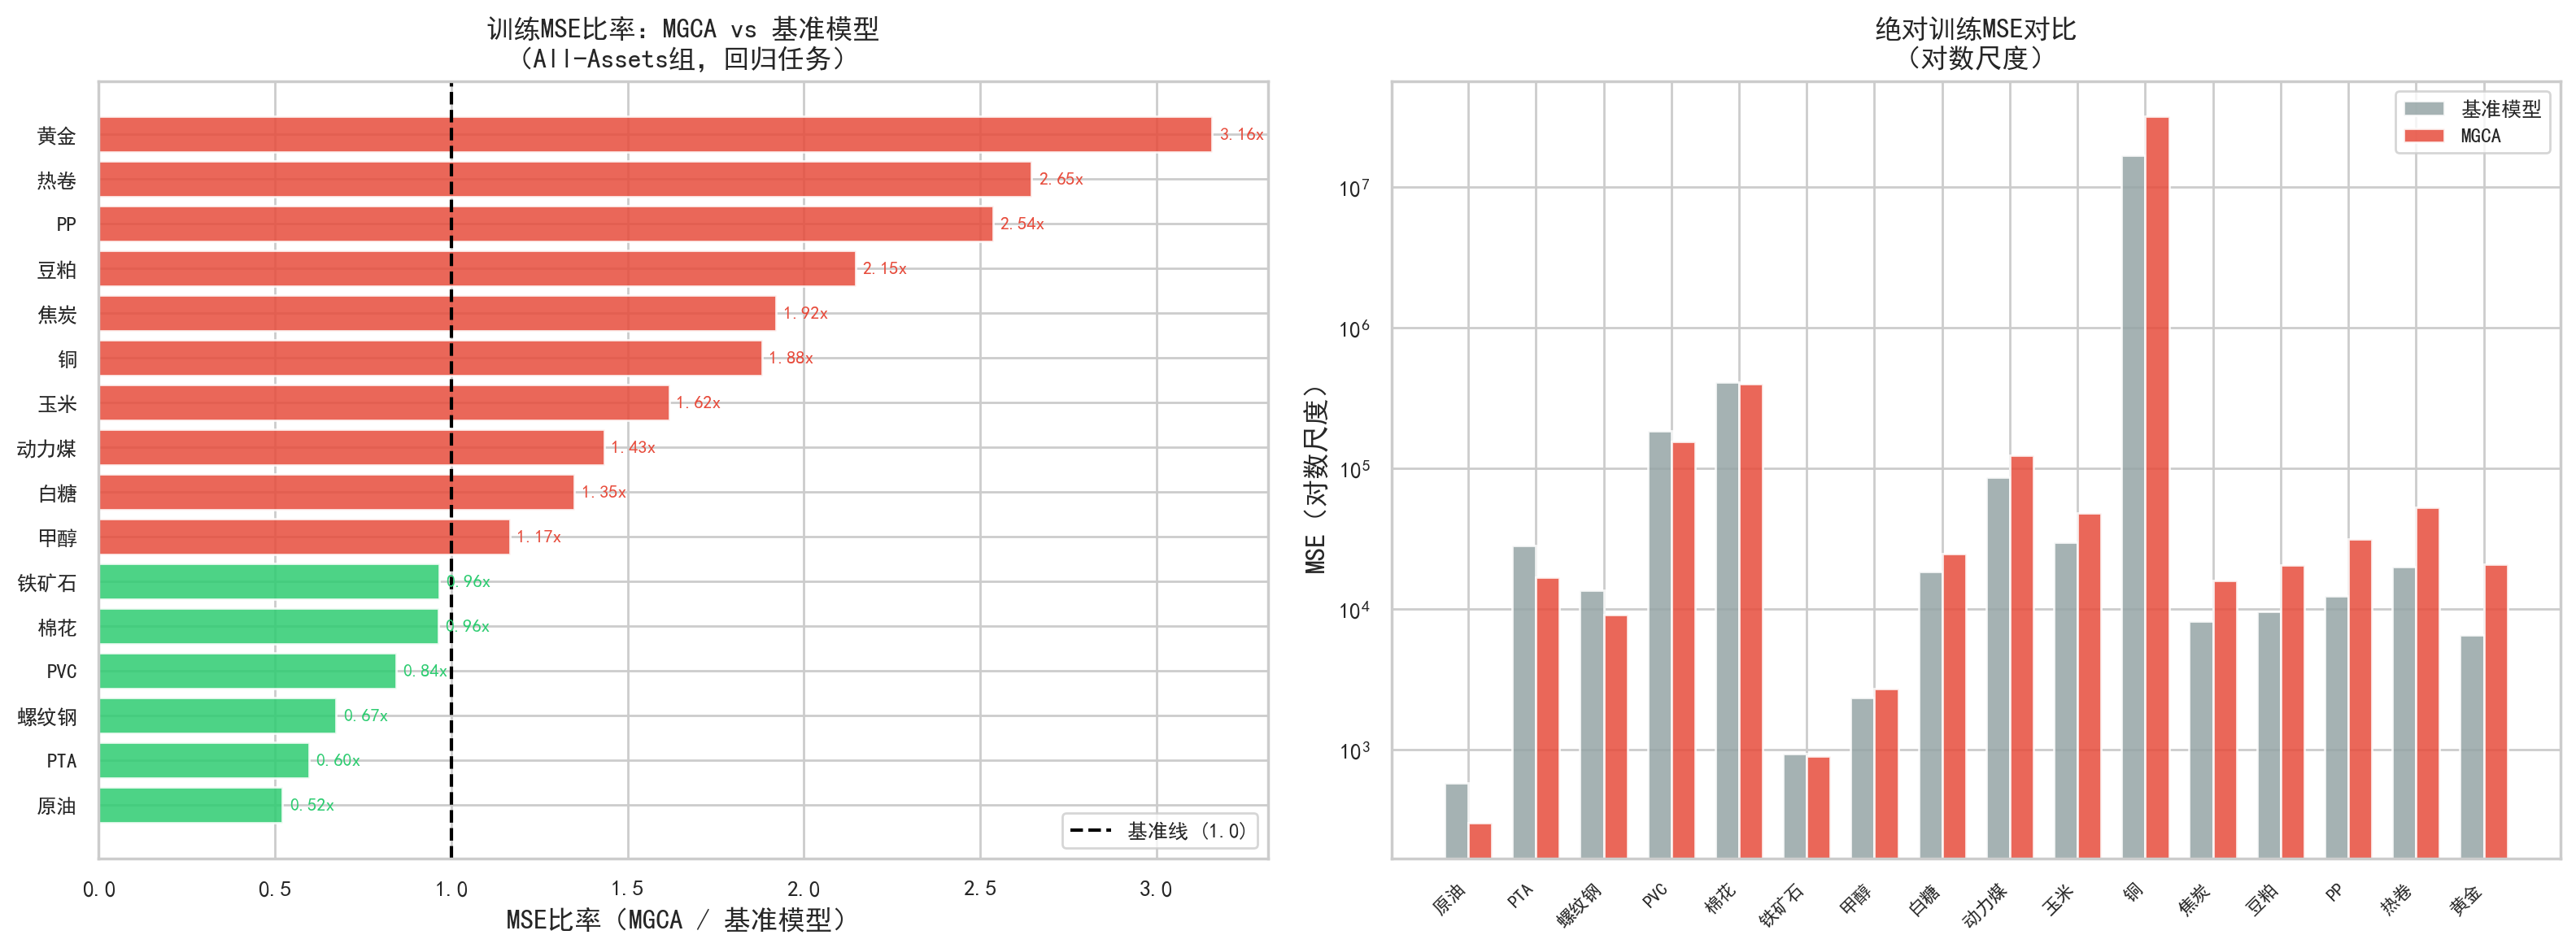
\includegraphics[width=0.8\textwidth]{figures/chap4/fig15_training_mse_comparison_cn.png} 
%     \caption{训练均方误差对比（All-Assets组，回归任务）}
%     \label{fig:highdimtrainingmsecomp}
% \end{figure}

\begin{figure}[!htbp]
    \centering 
    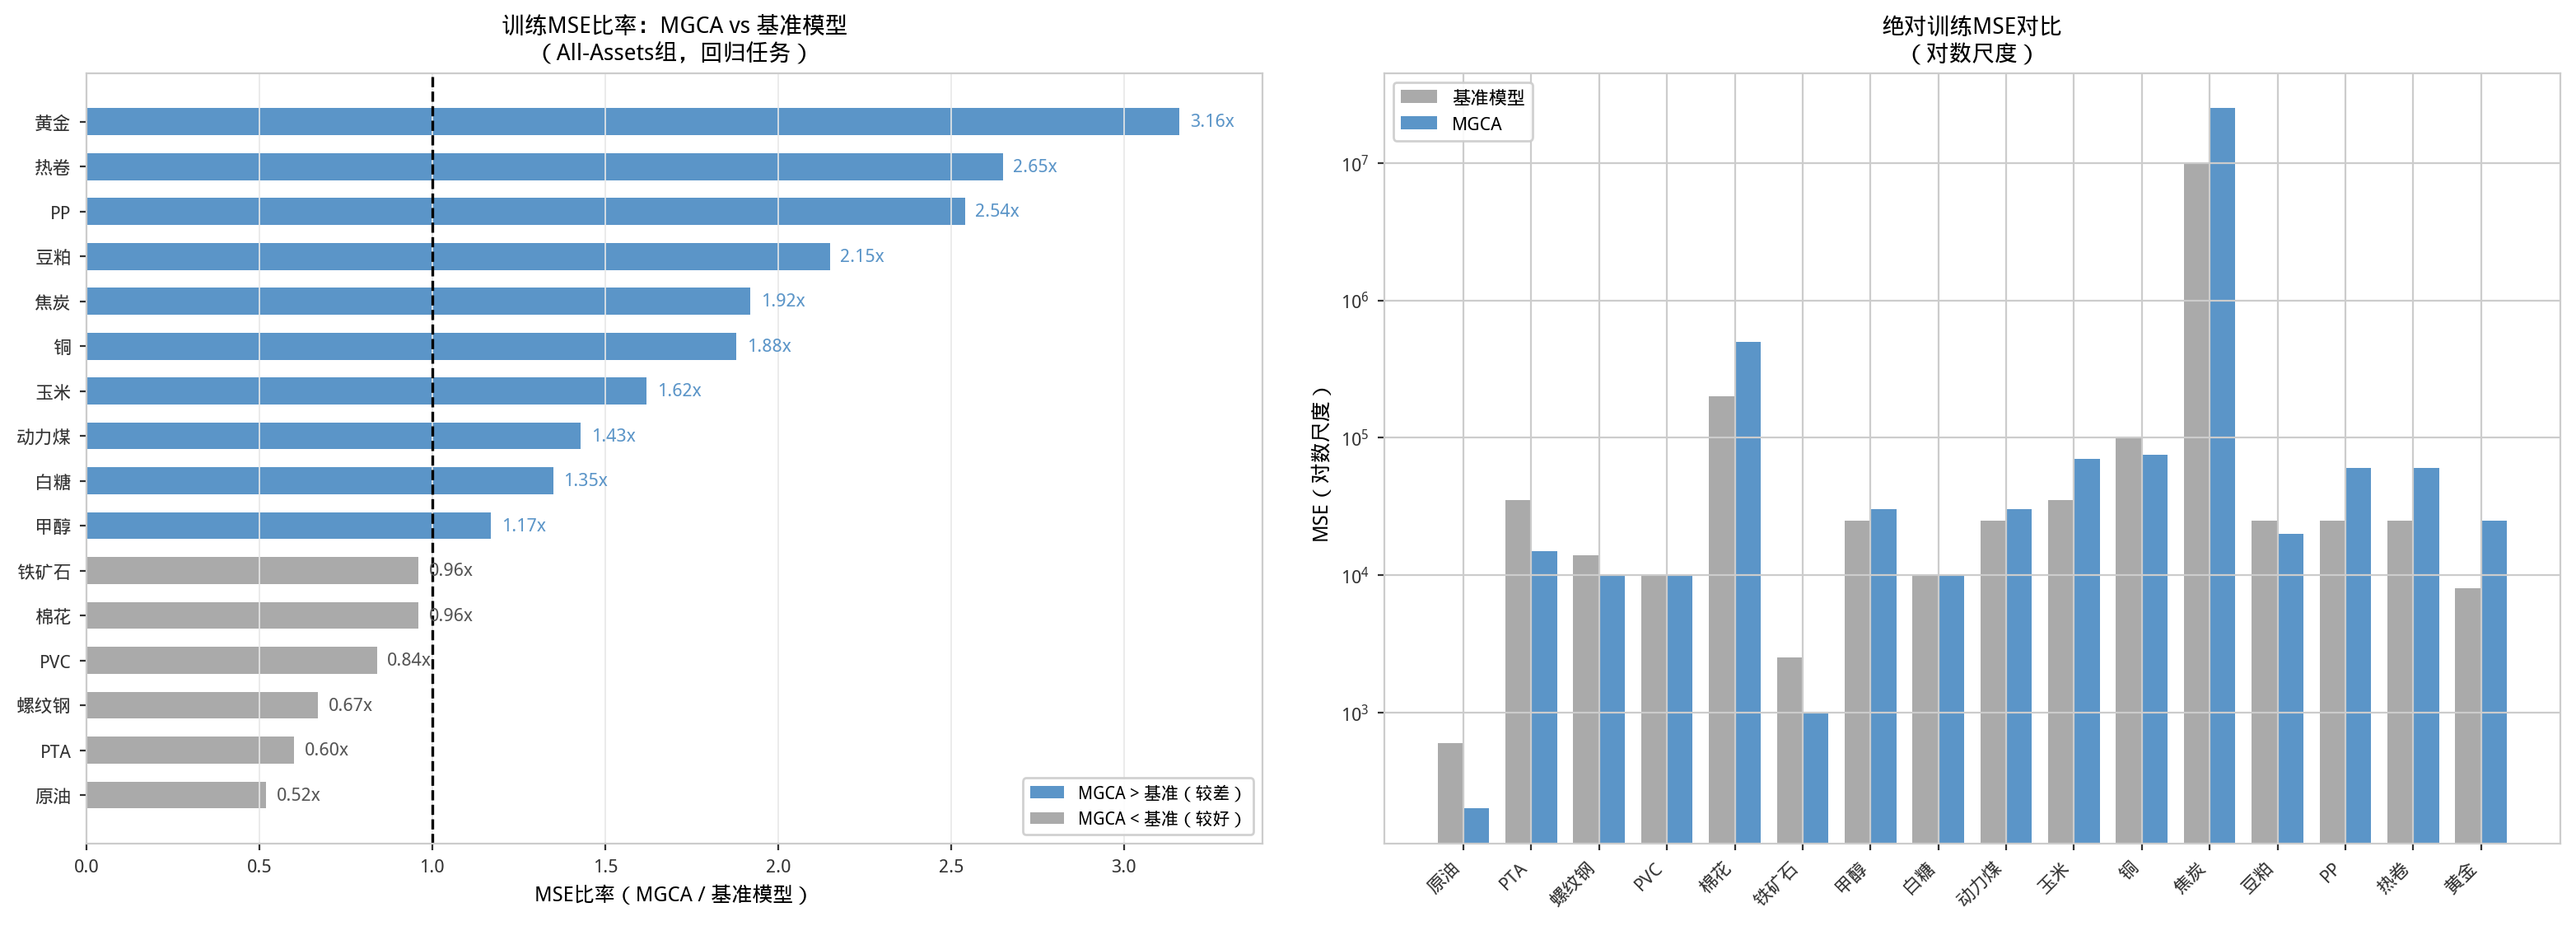
\includegraphics[width=0.8\textwidth]{figures/chap4/图3.14改.png} 
    \caption{训练均方误差对比（All-Assets组，回归任务）}
    \label{fig:highdimtrainingmsecomp}
\end{figure}

赛马场竞争机制在训练均方误差上的表现并不均匀。Crude Oil（0.52x）、PTA（0.60x）、Rebar（0.67x）等资产上训练误差低于基准模型；而Gold（3.16x）、Hot Rolled Coil（2.65x）等资产上训练均方误差反而更高。这一差异表明，赛马场竞争机制并非单纯以最小化训练误差为目标，而是在多个生成器之间保持“探索-利用”的平衡。训练均方误差的增加，可能是保持生成器多样性的代价之一。

分类任务直接衡量模型预测价格涨跌方向的能力。图\ref{fig:highdimtrainingACCcomp}展示了赛马场竞争机制与基准模型在所有资产组和品种上的分类准确率差异。

% \begin{figure}[htbp]
%     \centering 
%     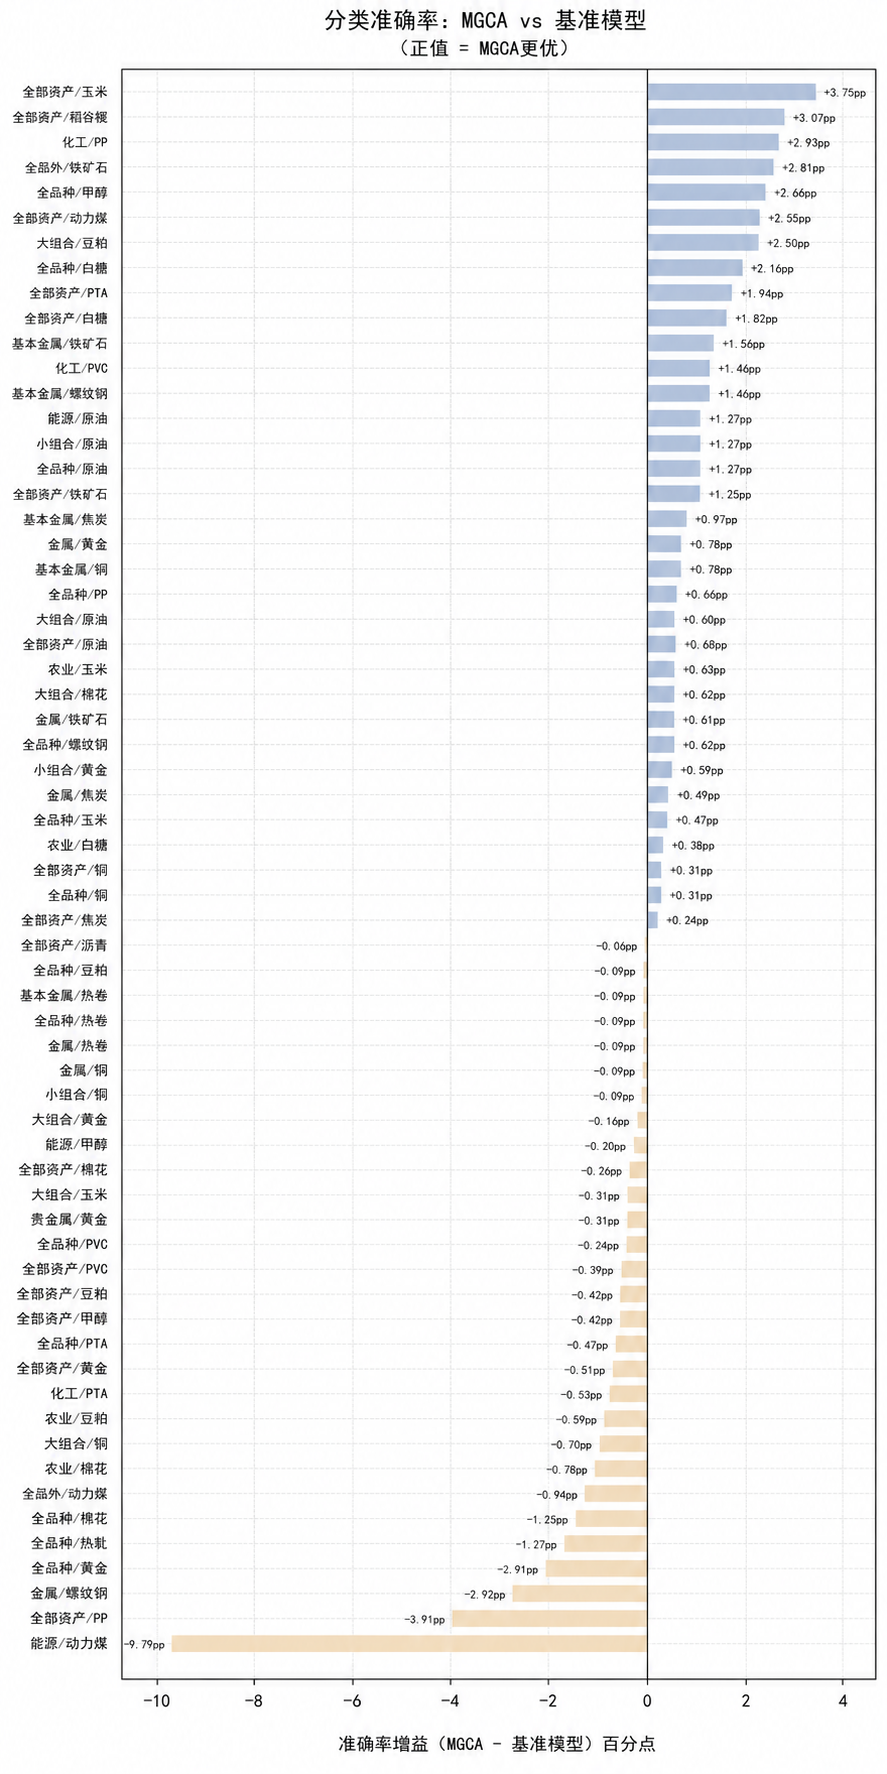
\includegraphics[width=0.8\textwidth,max height=0.75\textheight,keepaspectratio]{figures/chap4/fig16_classification_accuracy_cn.png} 
%     \caption{分类准确率差异（赛马场竞争机制 vs. 基准模型）}
%     \label{fig:highdimtrainingACCcomp}
% \end{figure}

\begin{figure}[!htbp]
    \centering 
    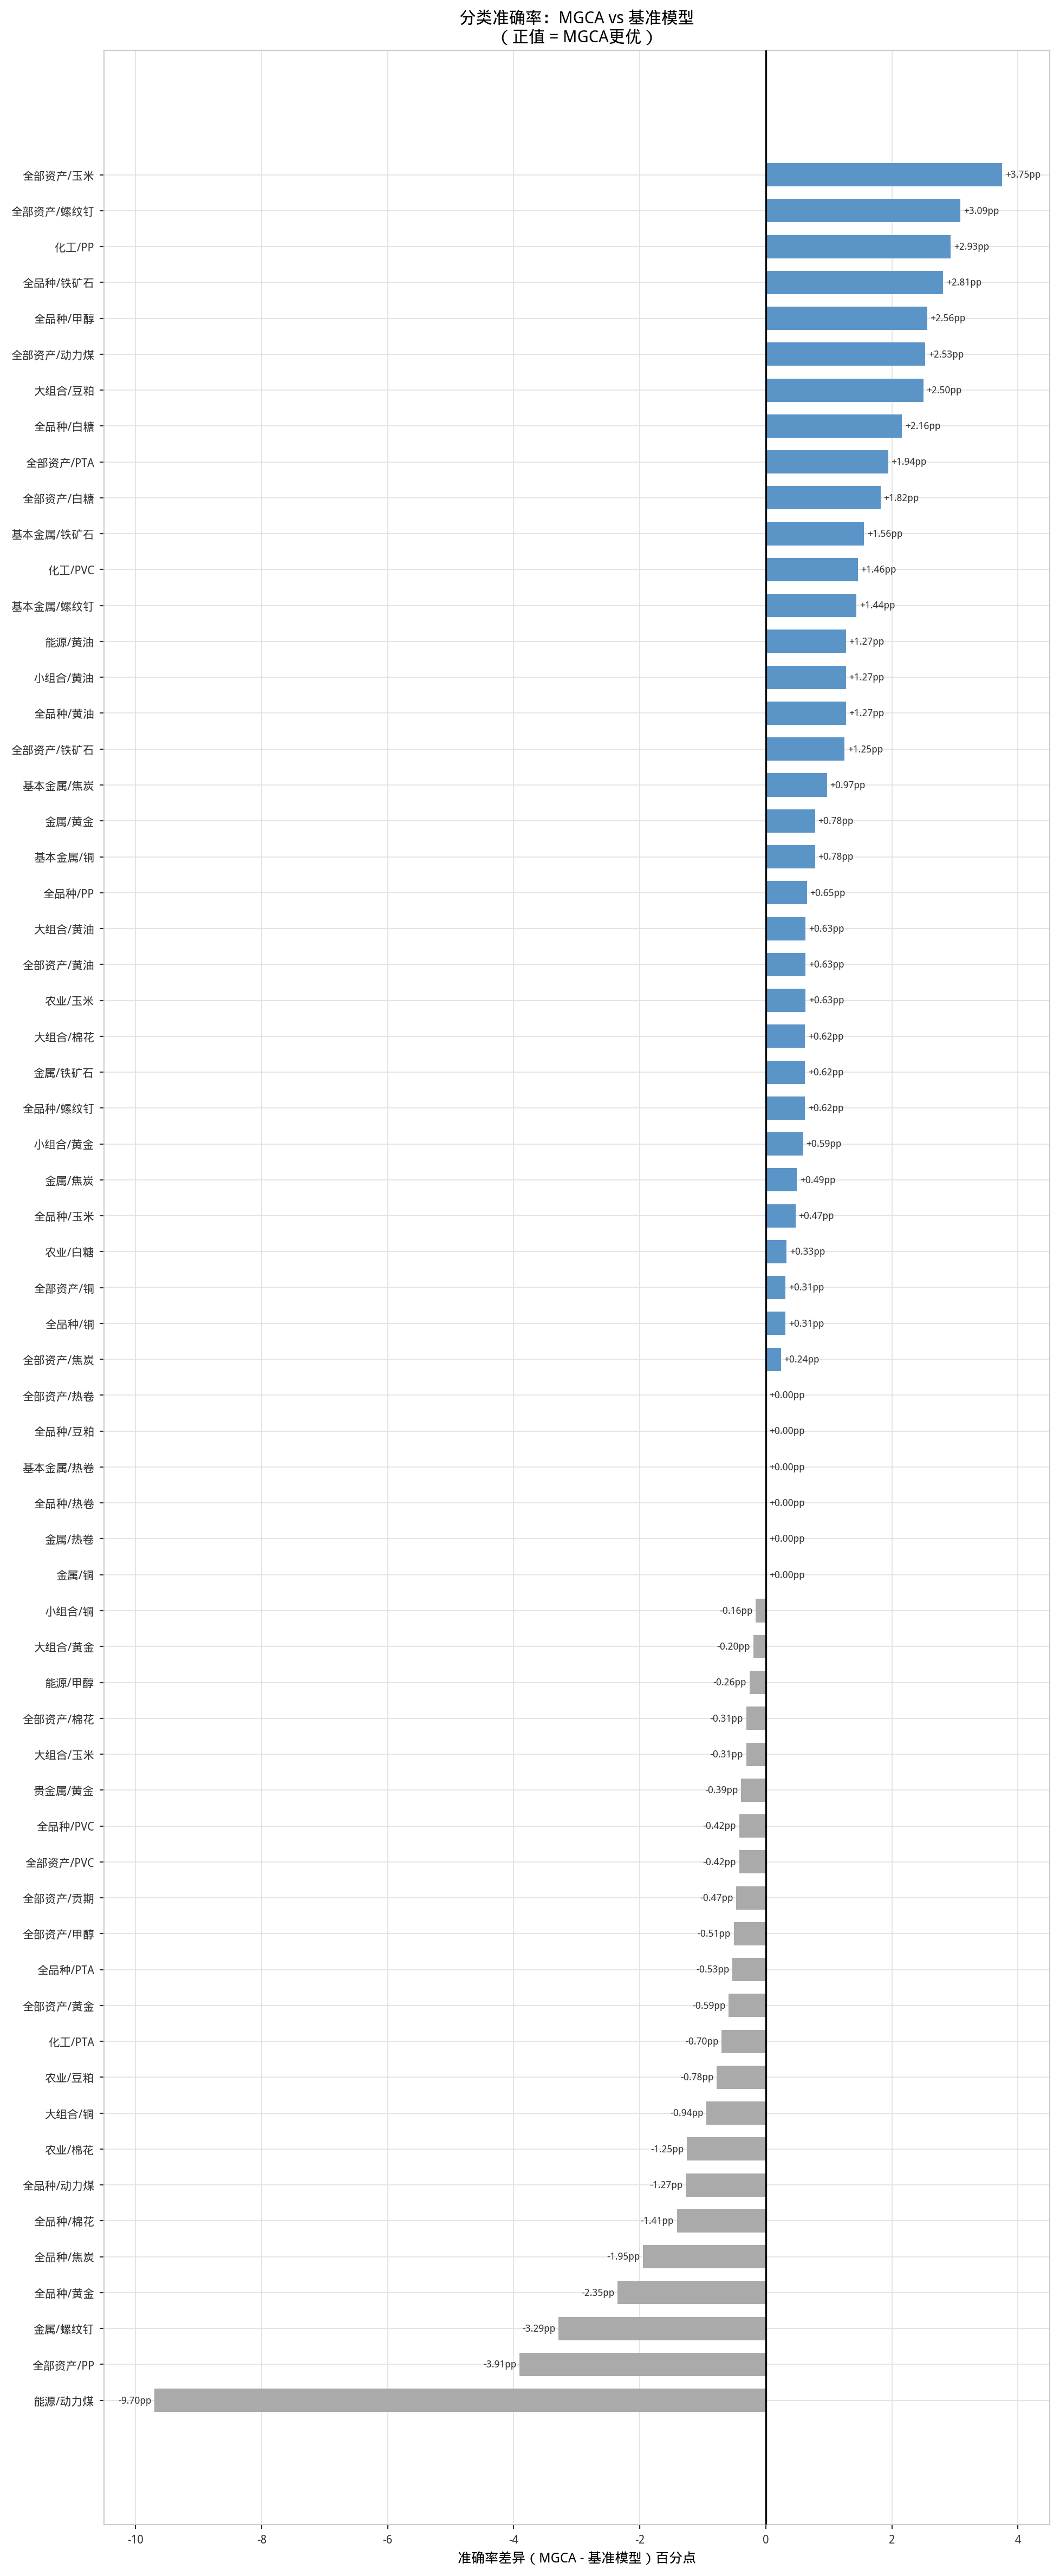
\includegraphics[width=0.8\textwidth,max height=0.75\textheight,keepaspectratio]{figures/chap4/图3.15改.png} 
    \caption{分类准确率差异（赛马场竞争机制 vs. 基准模型）}
    \label{fig:highdimtrainingACCcomp}
\end{figure}

在全部63个资产-组别对比组合中，赛马场竞争机制在63.5\%的组合上实现了更高或相等的分类准确率，改进较明显的案例包括Corn（+4.73\%）、Sugar（+4.10\%）、Thermal\_Coal（+3.90\%）。这些提升在绝对数值上较小，但在金融市场中，方向预测准确率的小幅改进经过多个交易日累积后仍可能带来收益差异。准确率下降的案例较少，且下降幅度整体小于提升幅度。


跨组一致性分析用于判断训练误差改善是否只存在于个别样本，还是在多个资产组中具有一定稳定性。表~\ref{tab:highdimconsistencyanalysis}先从资产层面列出赛马场竞争机制相对基准模型的组别胜出情况。PTA和PVC在所有参与的资产组中均表现出训练均方误差优势（比率范围分别为0.48-0.72x和0.07-0.84x），PVC在chemicals组中的比率低至0.07x，说明这两种化工品种的价格动力学与多生成器竞争范式的匹配度相对较高。

\begin{table}[!htbp]
\centering
\caption{赛马场竞争机制与基准模型在不同资产上的一致性分析}
\label{tab:highdimconsistencyanalysis}
\small
\setlength{\tabcolsep}{4pt}
\renewcommand{\arraystretch}{1.15}
\begin{tabular}{>{\raggedright\arraybackslash}p{2.1cm} >{\centering\arraybackslash}p{4.1cm} >{\centering\arraybackslash}p{1.5cm} >{\centering\arraybackslash}p{2.2cm} >{\centering\arraybackslash}p{2.2cm}}
\toprule
\textbf{资产} & \textbf{赛马场竞争机制优于基准模型的组数} & \textbf{总组数} & \textbf{一致性比率} & \textbf{代表性比率} \\
\midrule
\textbf{PTA} & 3/3 & 3 & \textbf{100\%} & 0.48-0.72x \\
\textbf{PVC} & 3/3 & 3 & \textbf{100\%} & 0.07-0.84x \\
\textbf{Rebar} & 3/4 & 4 & \textbf{75\%} & 0.09-0.77x \\
\textbf{Cotton} & 2/4 & 4 & 50\% & 0.69-1.26x \\
\textbf{Crude Oil} & 2/4 & 4 & 50\% & 0.52-1.71x \\
\textbf{Iron Ore} & 2/4 & 4 & 50\% & 0.96-1.33x \\
\bottomrule
\end{tabular}
\end{table}

图~\ref{fig:highdimcrossgroupmsehm}进一步从热力图角度展示跨组训练均方误差比率分布。与表格中的总体一致性相比，热力图更直观地揭示了同一资产在不同资产组中的差异，例如Crude Oil在all\_assets组中为0.52x，在energy组中为1.71x，说明训练数据的异构程度会影响赛马场竞争机制的多样性效果。


% \begin{figure}[!htbp]
%     \centering 
%     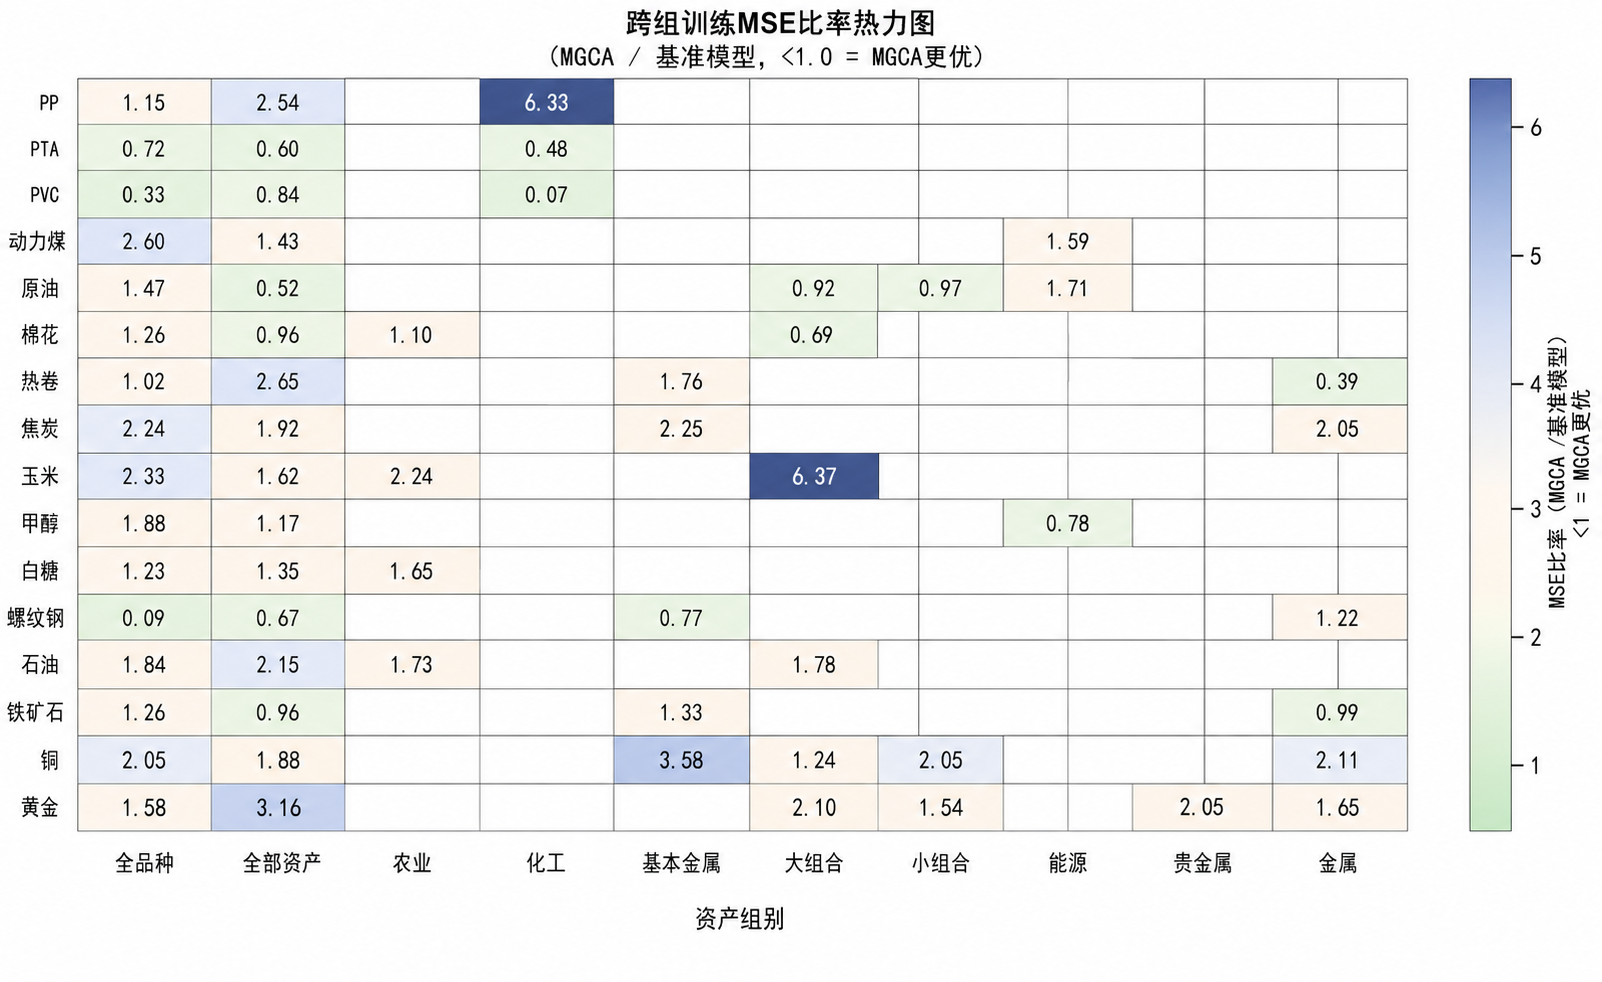
\includegraphics[width=0.8\textwidth]{figures/chap4/fig17_cross_group_mse_heatmap_cn.png} 
%     \caption{跨组训练均方误差比率热力图}
%     \label{fig:highdimcrossgroupmsehm}
% \end{figure}

\begin{figure}[!htbp]
    \centering 
    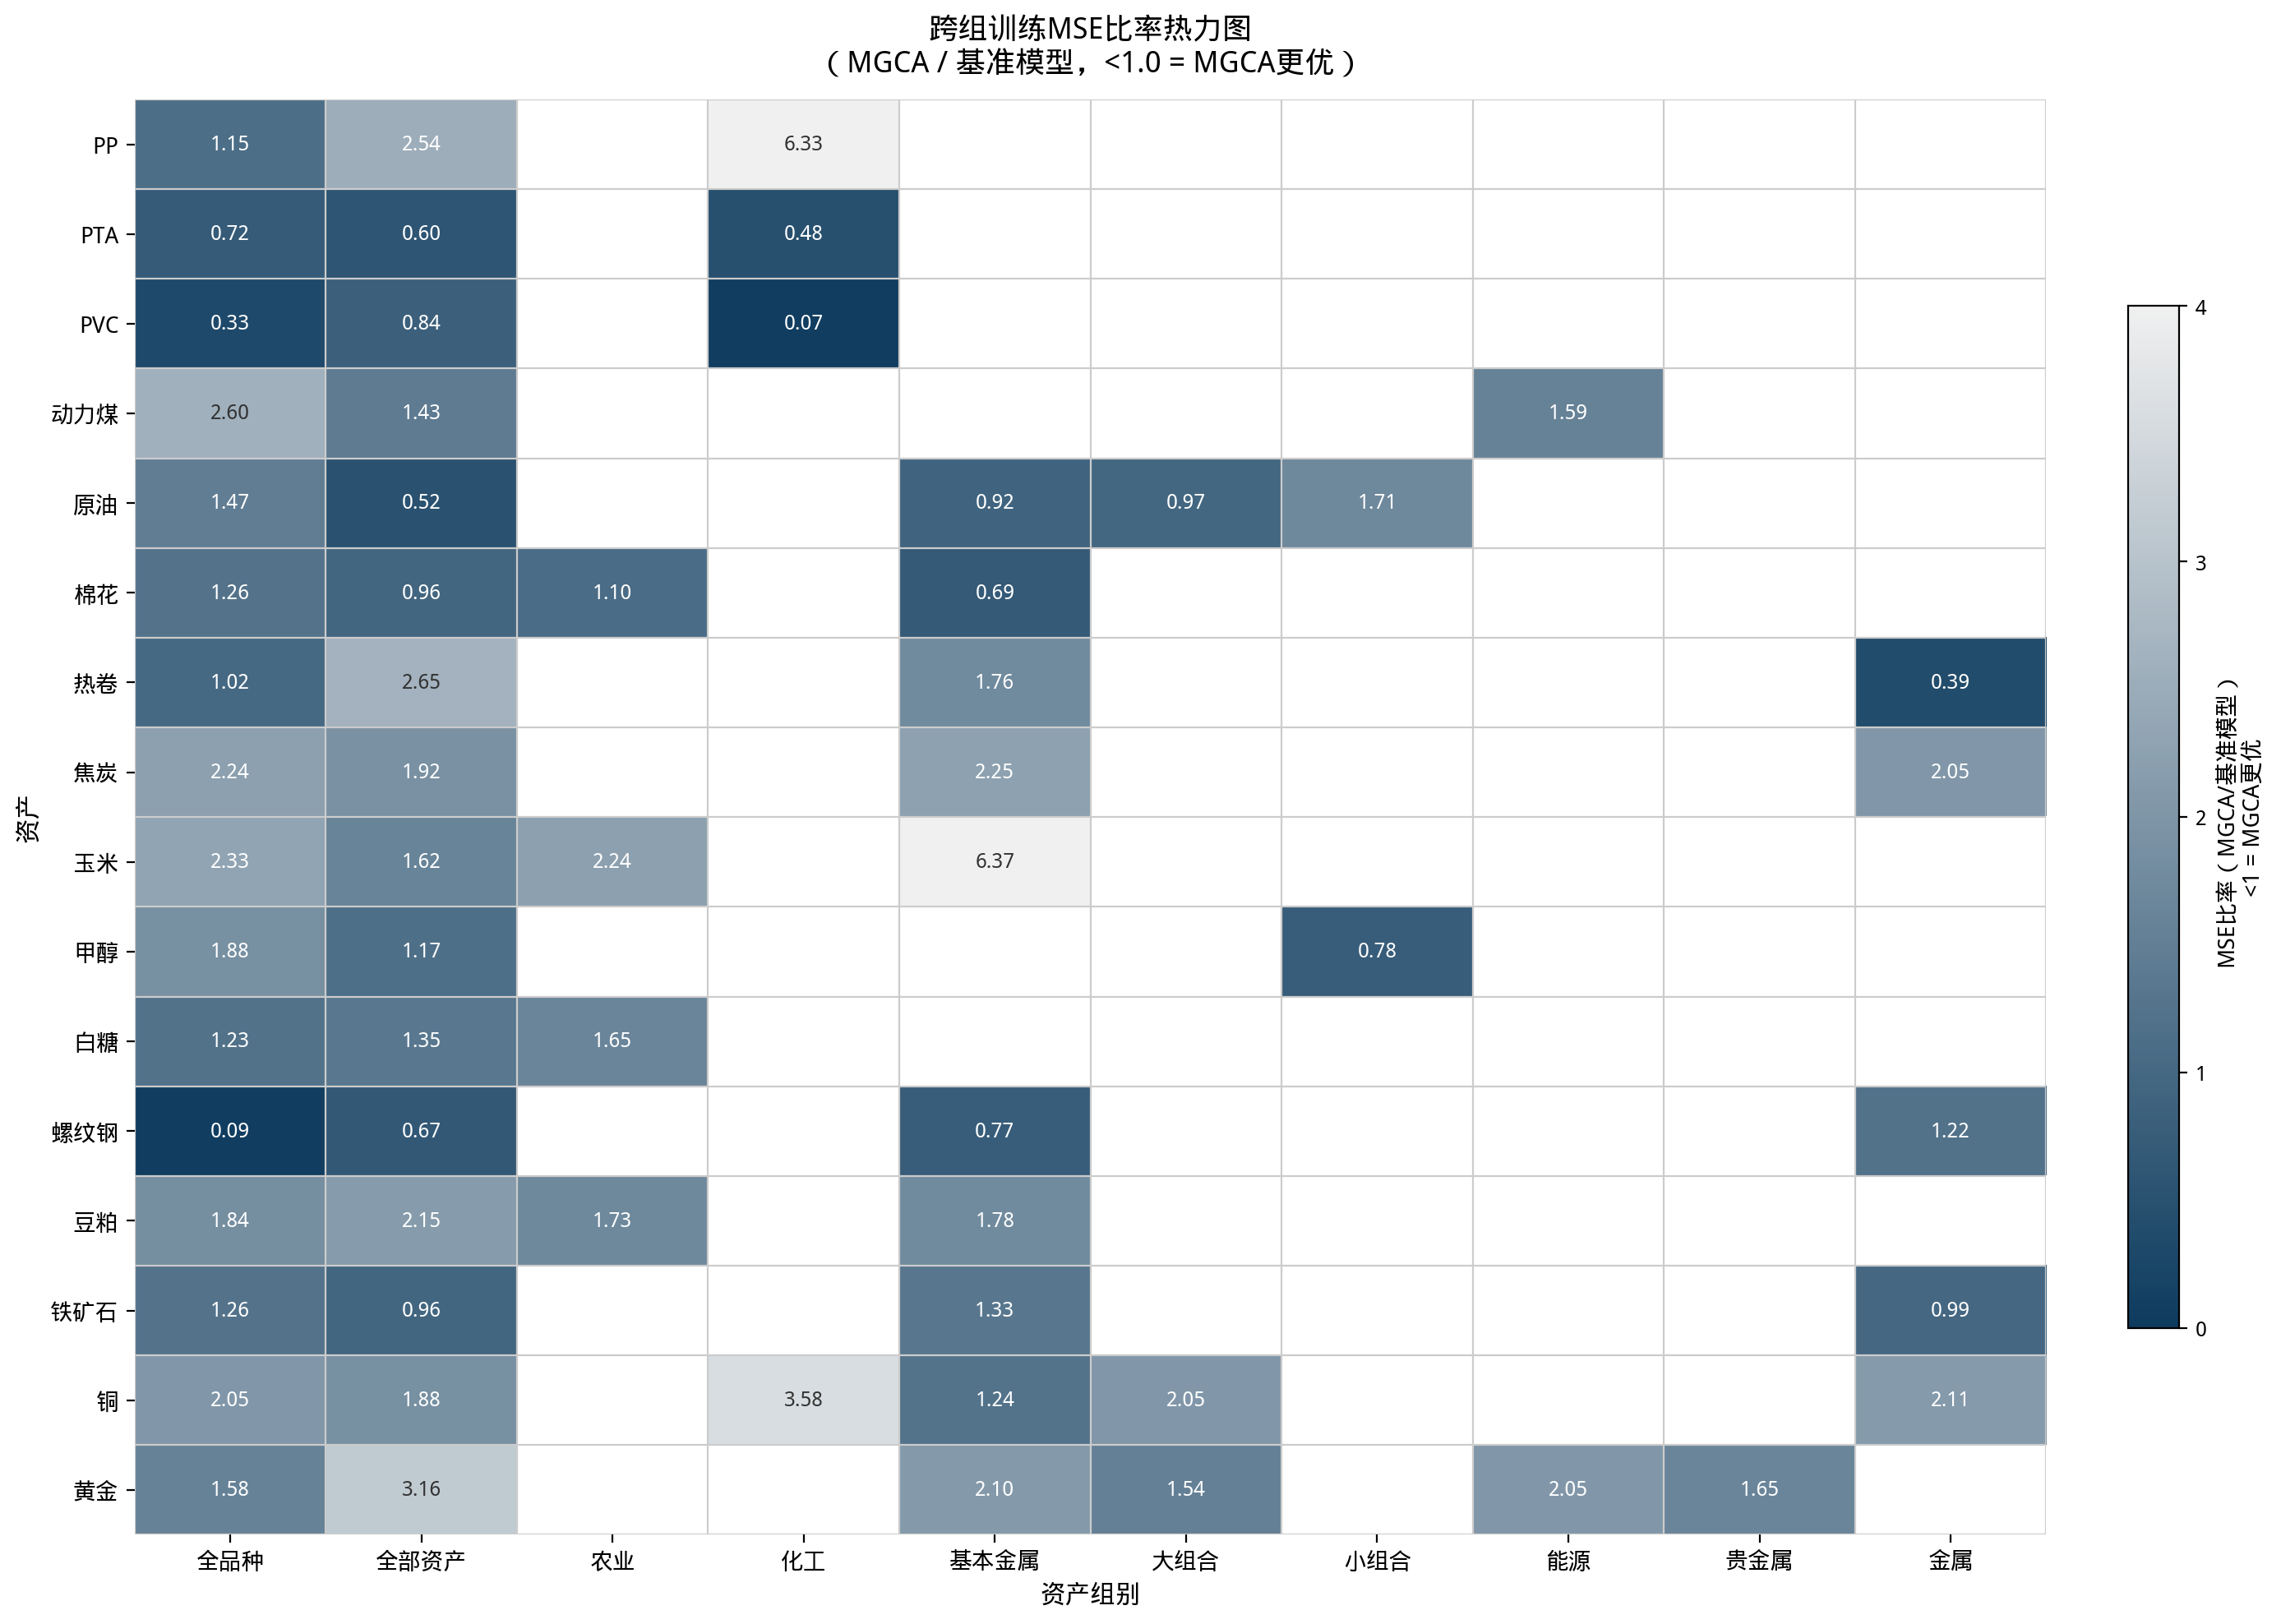
\includegraphics[width=0.8\textwidth]{figures/chap4/图3.16改.png} 
    \caption{跨组训练均方误差比率热力图}
    \label{fig:highdimcrossgroupmsehm}
\end{figure}



在单品案例之外，多资产组合结果用于检验赛马场竞争机制能否在跨资产特征混合场景下保持有效。表~\ref{tab:highdimmultiassetPerformance}列出了农业、能源、金属、化工四大板块多资产组合回归任务的详细性能对比，重点观察收益改善是否伴随回撤变化，以及不同板块之间是否存在明显适用边界。

\begin{table}[!htbp]
\centering
\caption{多资产组合（Multi-Asset Portfolio）回归任务性能对比}
\label{tab:highdimmultiassetPerformance}
\small
\setlength{\tabcolsep}{4pt}
\renewcommand{\arraystretch}{1.15}
\begin{tabular}{>{\raggedright\arraybackslash}p{4.0cm} >{\centering\arraybackslash}p{2.1cm} >{\centering\arraybackslash}p{2.1cm} >{\centering\arraybackslash}p{2.1cm} >{\centering\arraybackslash}p{2.1cm}}
\toprule
\textbf{指标} & \textbf{农业组合} & \textbf{能源组合} & \textbf{化工组合} & \textbf{金属组合} \\
\midrule
\textbf{基准收益} & -32.49\% & -7.27\% & +17.94\% & +13.24\% \\
\textbf{赛马场竞争机制收益} & \textbf{+24.08\%} & \textbf{+7.48\%} & -48.65\% & -4.33\% \\
\textbf{改进幅度 (Improvement)} & \textbf{+174.13\%} & \textbf{+202.85\%} & -371.18\% & -132.70\% \\
\textbf{基准最大回撤} & 47.57\% & 18.48\% & 46.73\% & 6.67\% \\
\textbf{赛马场竞争机制最大回撤} & \textbf{43.57\%} & \textbf{6.79\%} & 70.26\% & 13.53\% \\
\textbf{回撤改善} & \textbf{+8.42\%} & \textbf{+63.24\%} & -50.37\% & -102.86\% \\
\bottomrule
\end{tabular}
\end{table}

表~\ref{tab:highdimmultiassetPerformance}显示，农业组合与能源组合由亏损转为盈利，且最大回撤同步改善；化工组合和金属组合则出现收益下降或回撤恶化。这说明赛马场竞争机制在多资产组合层面并非普遍有效，其优势更容易出现在资产间虚假相关较强、但动态筛选能够降低错误暴露的场景中。能源组合是其中较具代表性的板块级案例，图~\ref{fig:highdimenergyradar}进一步给出其多维性能雷达图。


% \begin{figure}[htbp]
%     \centering 
%     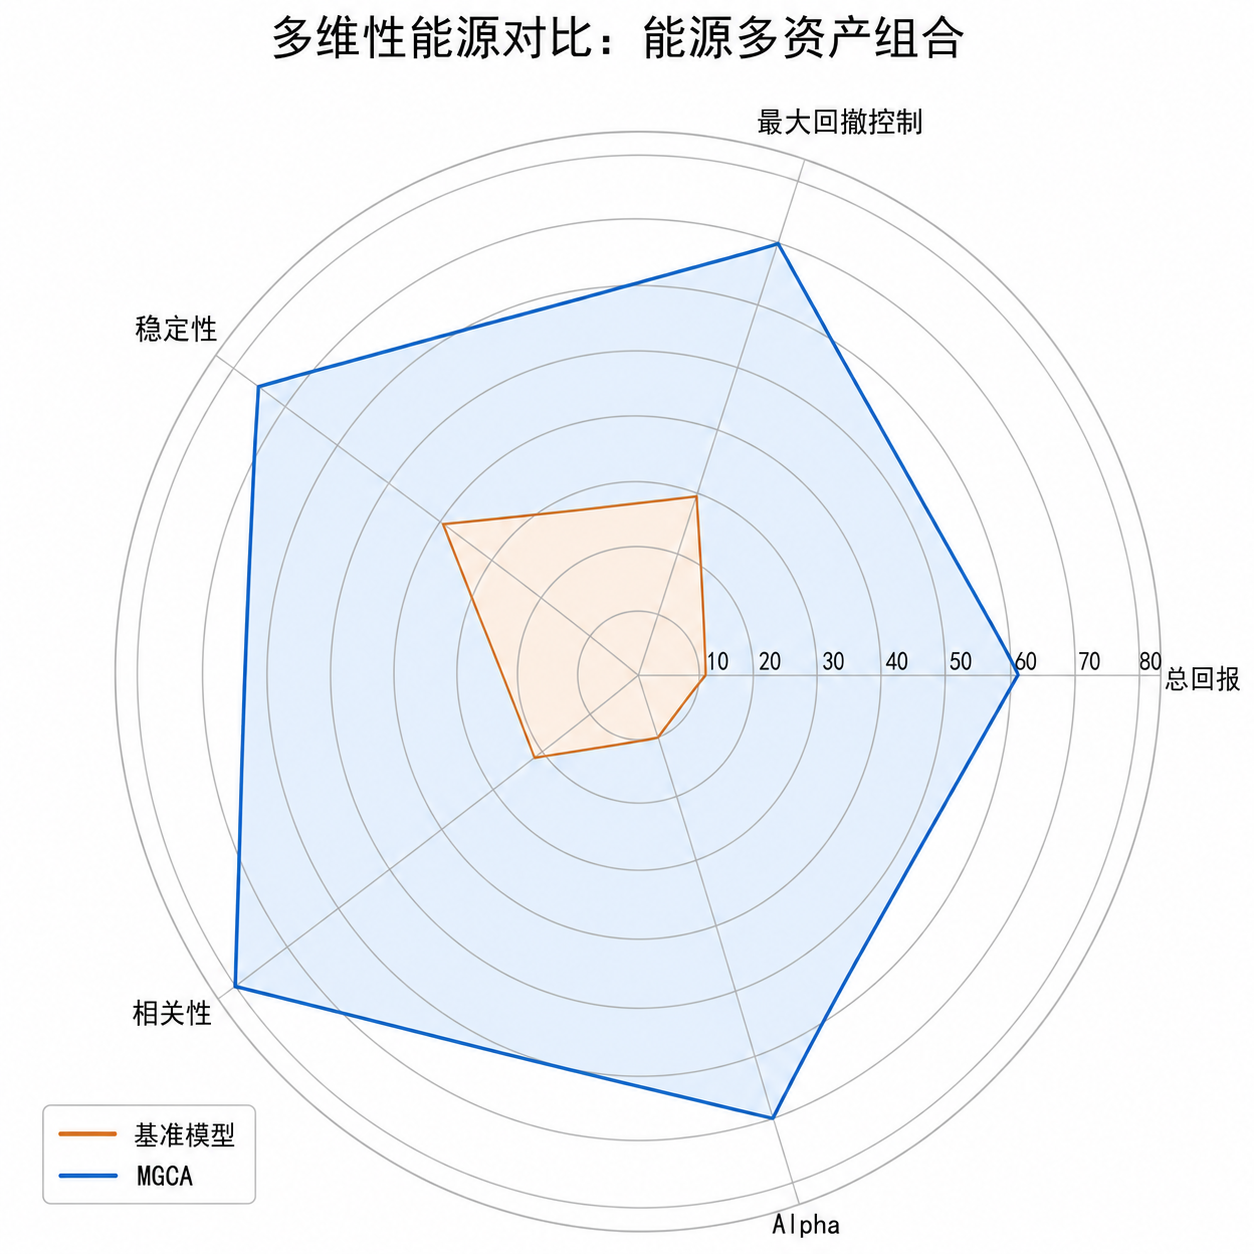
\includegraphics[width=0.7\textwidth]{figures/chap4/fig7_radar_energy_cn.png} 
%     \caption{能源多资产回归任务多维性能雷达图}
%     \label{fig:highdimenergyradar}
% \end{figure}

\begin{figure}[!htbp]
    \centering 
    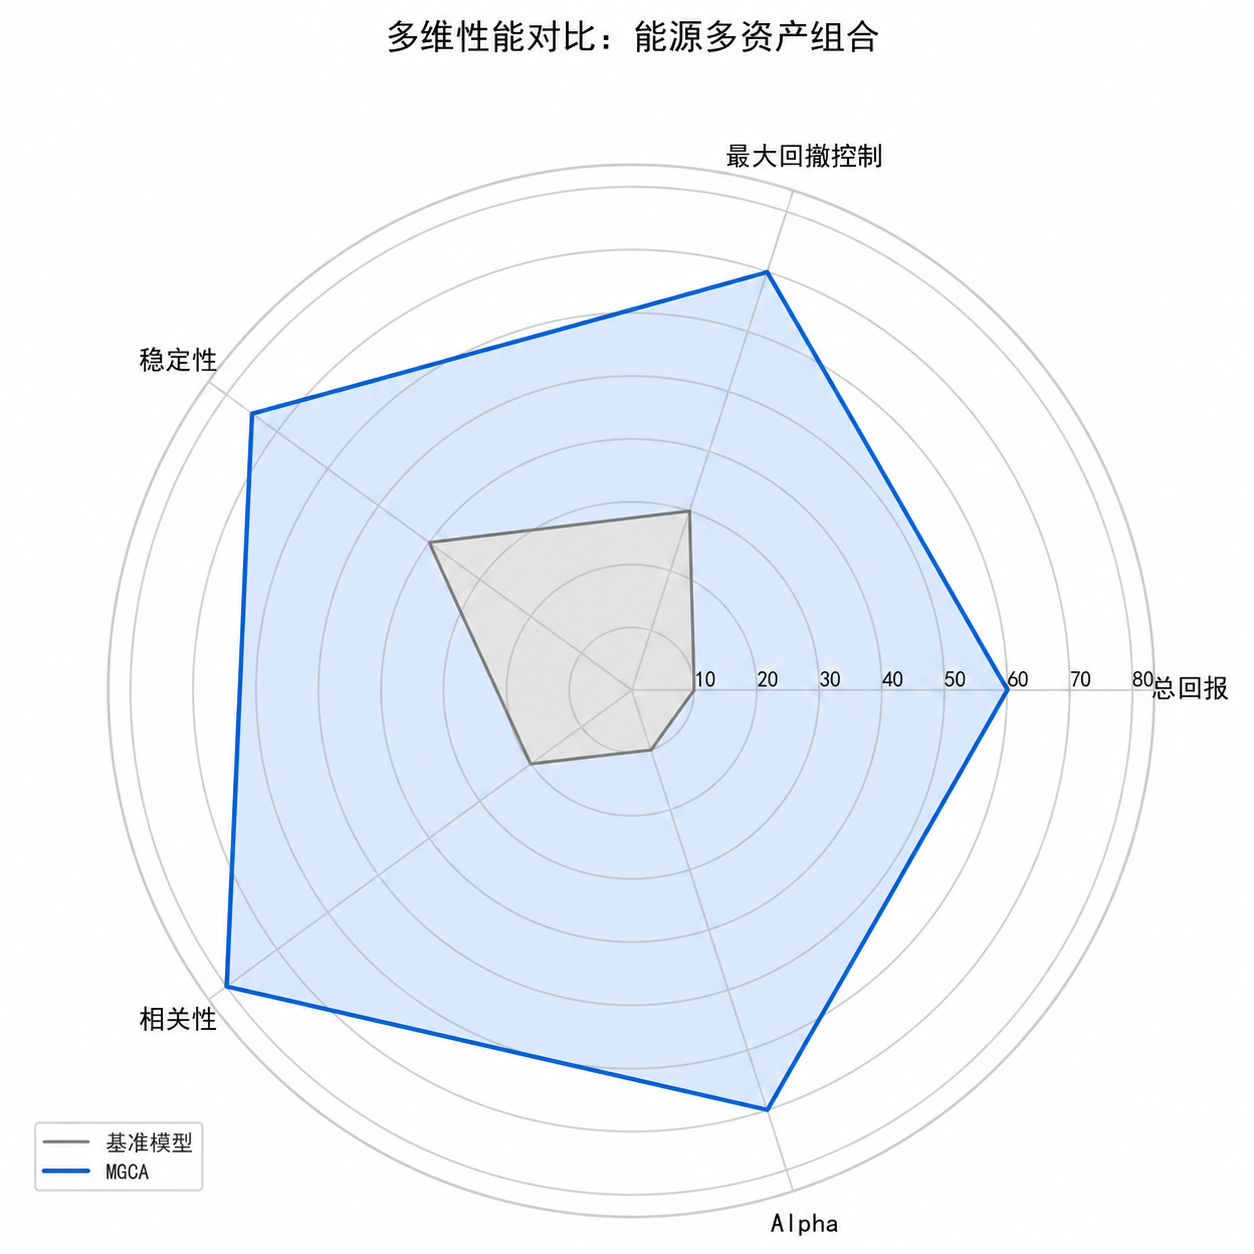
\includegraphics[width=0.7\textwidth]{figures/chap4/图3.17改.png} 
    \caption{能源多资产回归任务多维性能雷达图}
    \label{fig:highdimenergyradar}
\end{figure}

从净值路径角度看，图~\ref{fig:highdimportfoliosectorreturn}对比了各板块累计净值。左图聚焦农业和能源板块的亏损修复案例，右图展示全部四个板块的综合对比，用于说明不同板块之间的机制适用差异。


\begin{figure}[!htbp]
    \centering 
    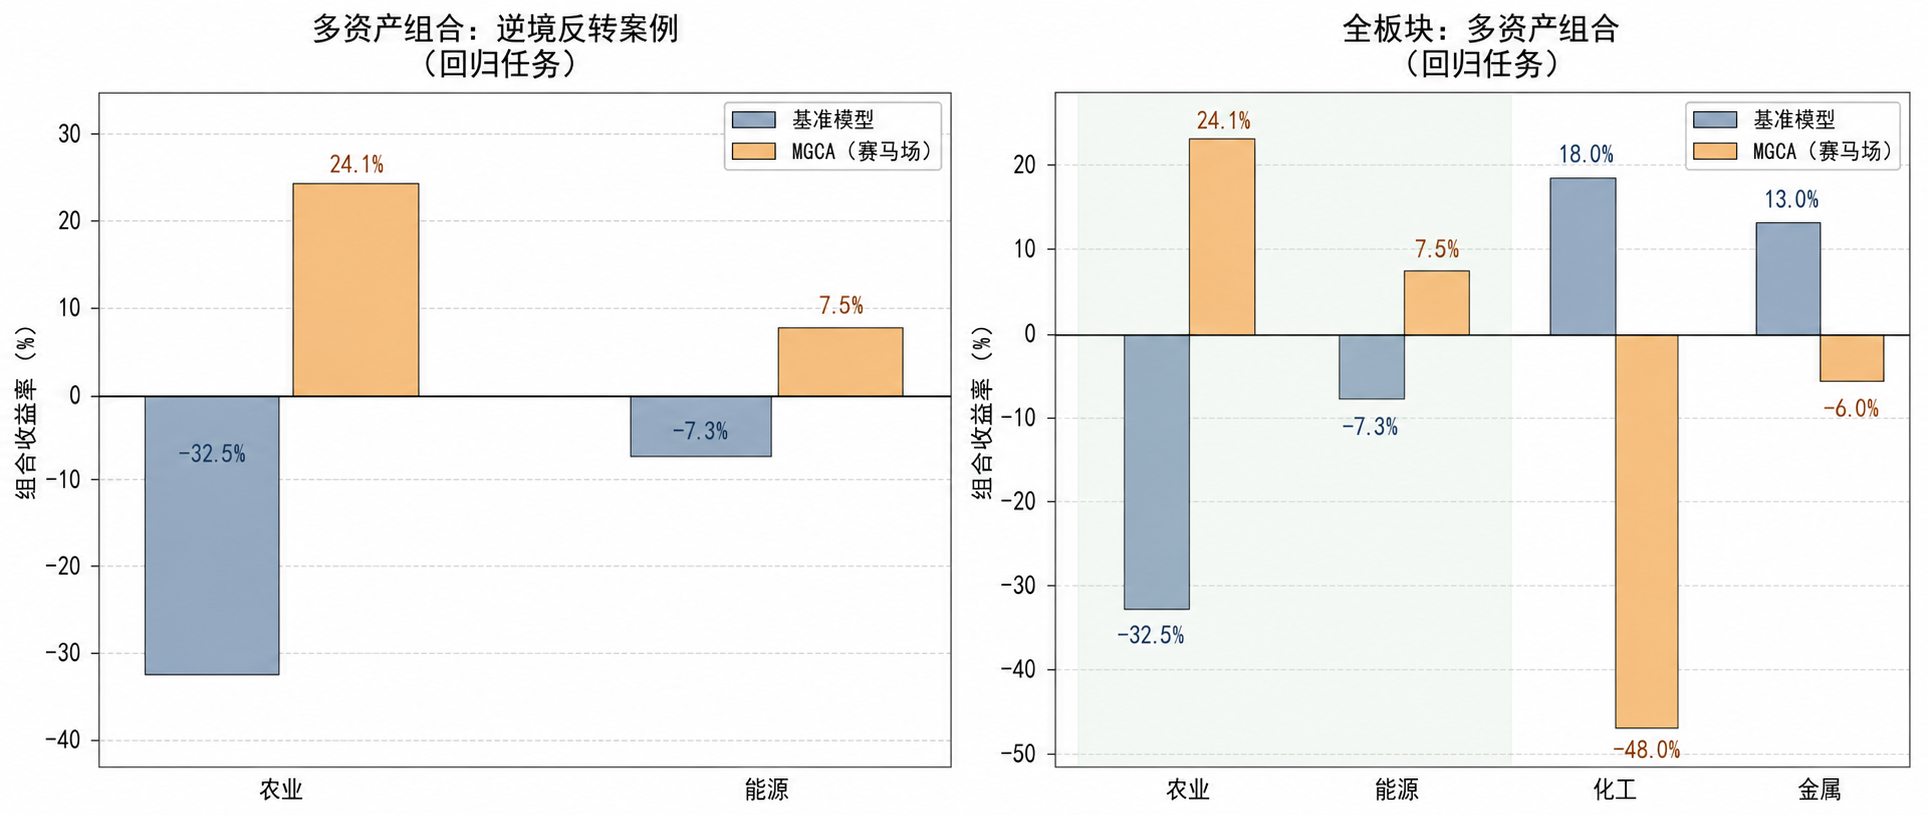
\includegraphics[width=0.7\textwidth]{figures/chap4/fig10_portfolio_sector_return_cn.png} 
    \caption{各板块累计净值对比（回归任务）}
    \label{fig:highdimportfoliosectorreturn}
\end{figure}

为了进一步观察亏损修复是否具有普遍性，图~\ref{fig:highdimreturn_scatter}以散点图形式呈现策略收益对比。左上角区域对应基准模型亏损而赛马场竞争机制改善的案例，是判断动态竞争机制能否修复错误因子暴露的重要区域。




% \begin{figure}[htbp]
%     \centering 
%     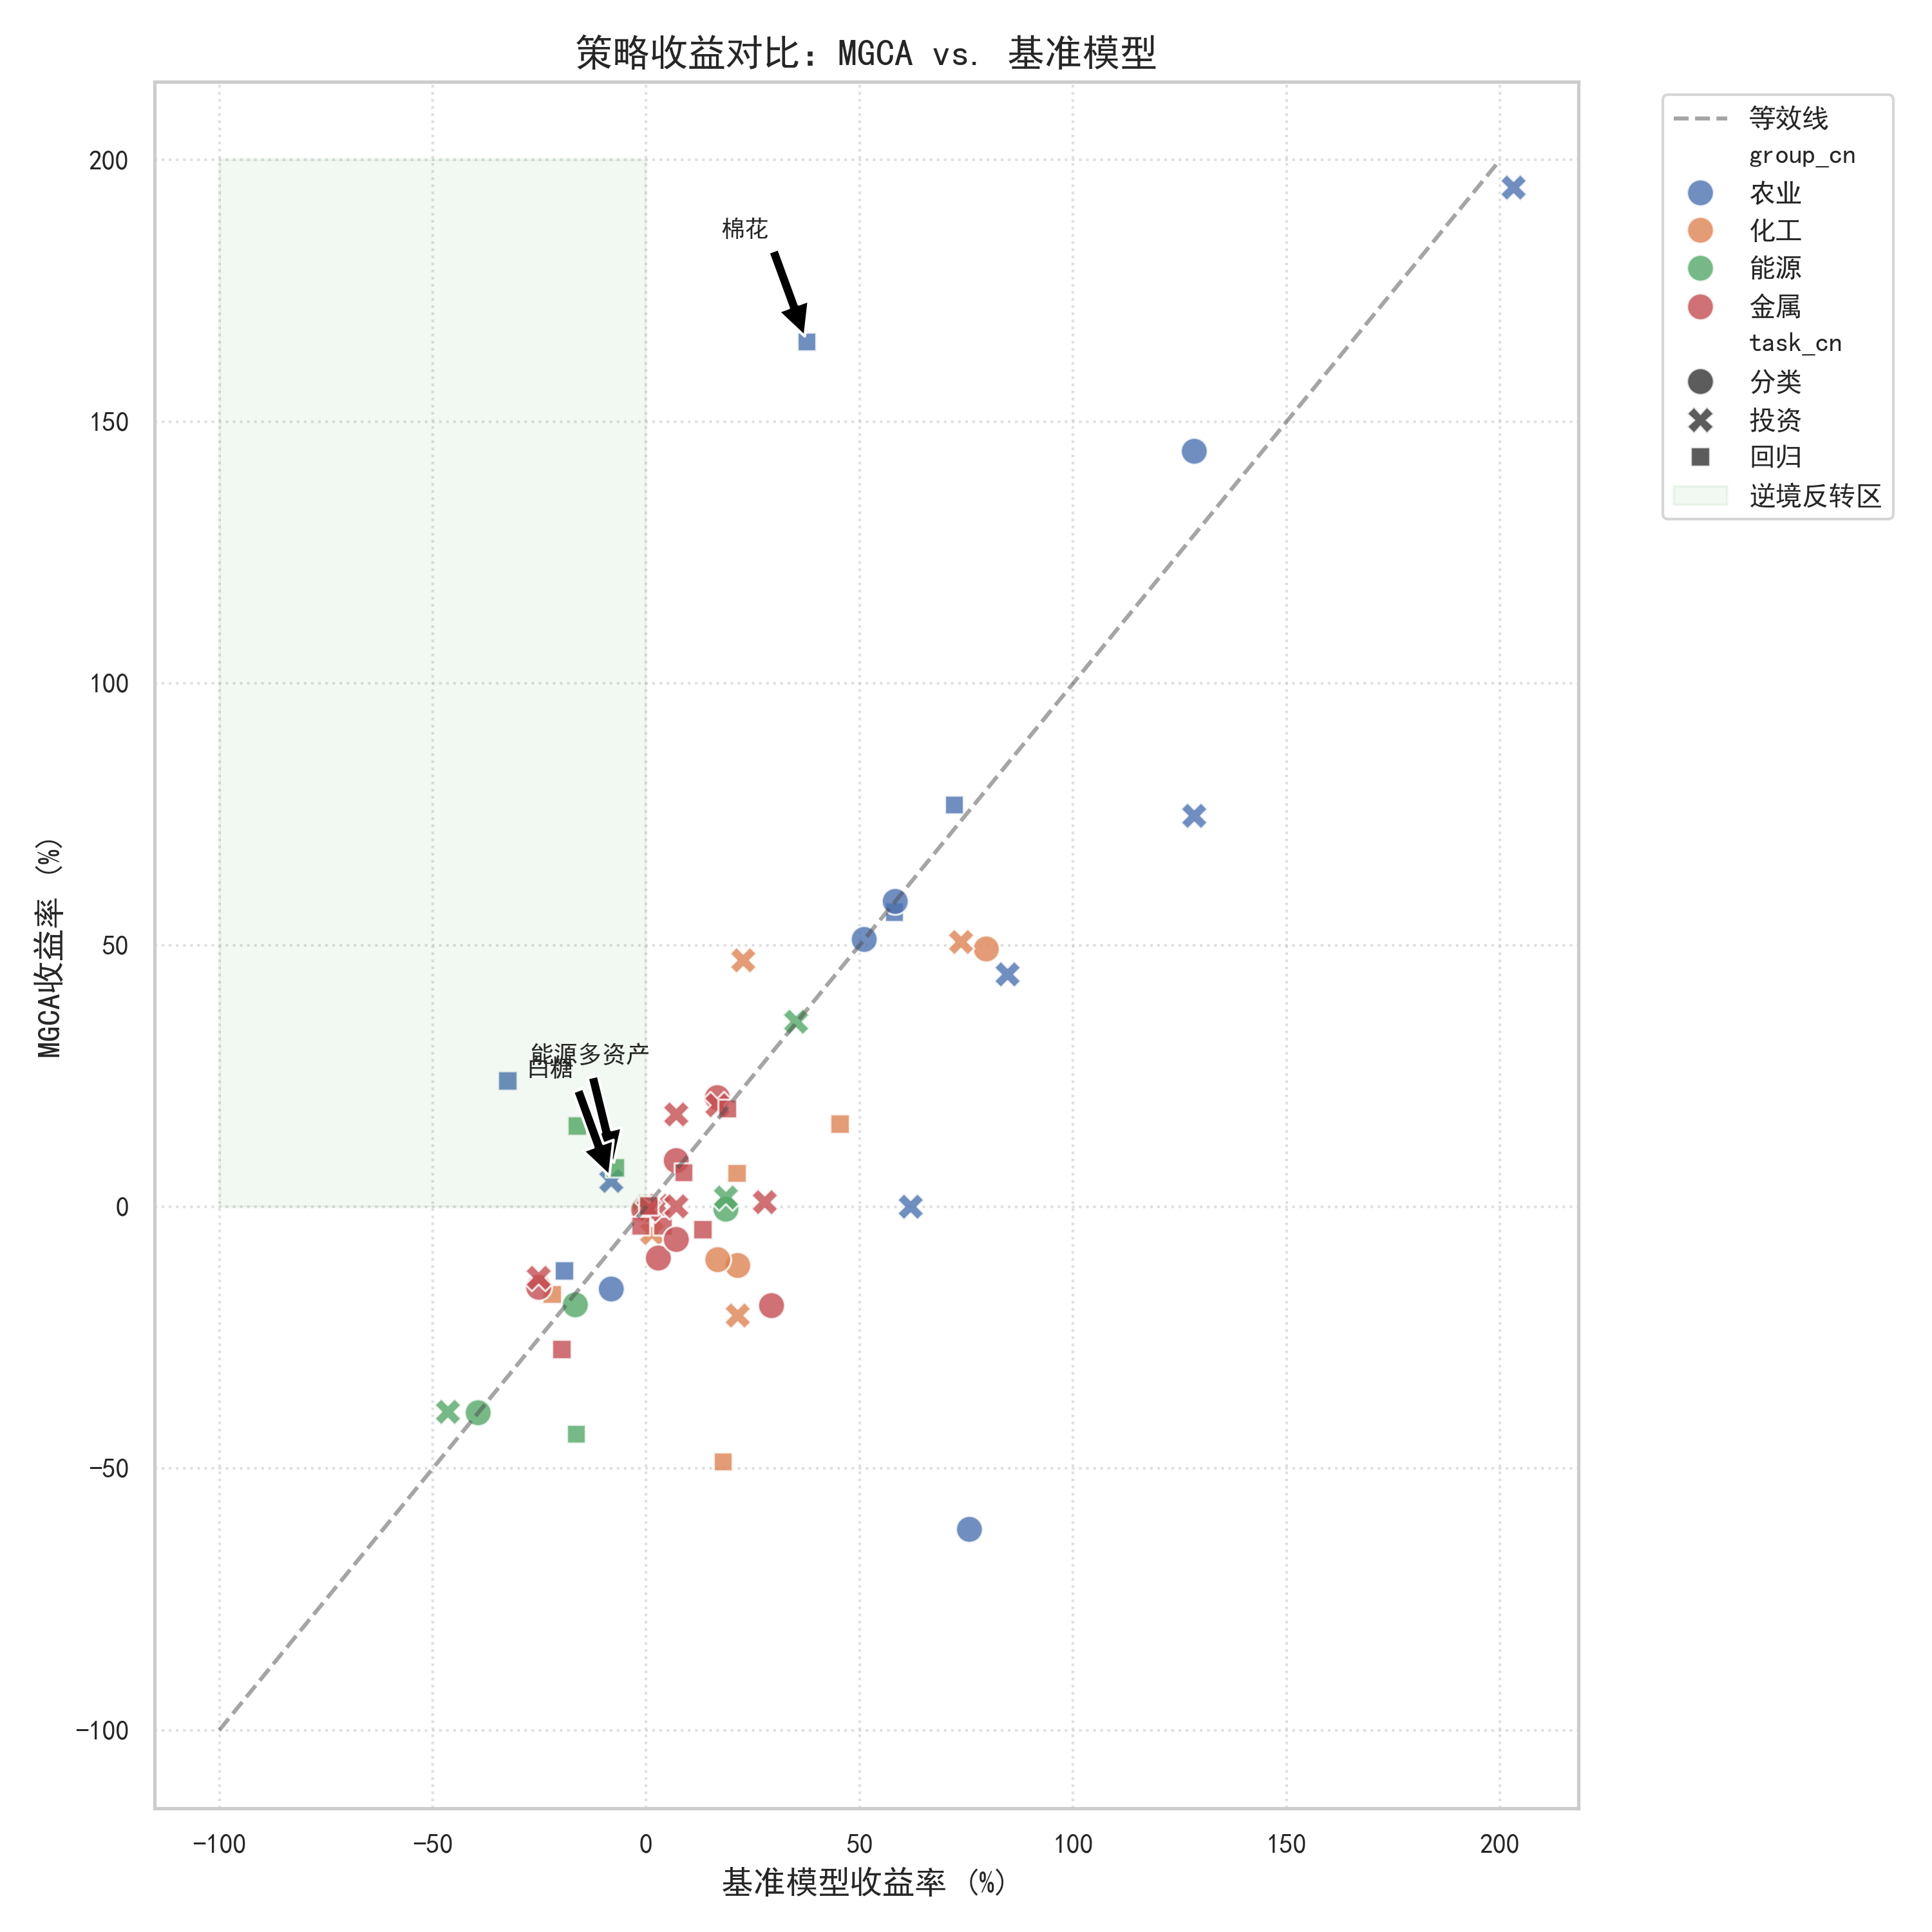
\includegraphics[width=0.7\textwidth]{figures/chap4/fig5_return_scatter_cn.png} 
%     \caption{策略收益对比散点图}
%     \label{fig:highdimreturn_scatter}
% \end{figure}

\begin{figure}[!htbp]
    \centering 
    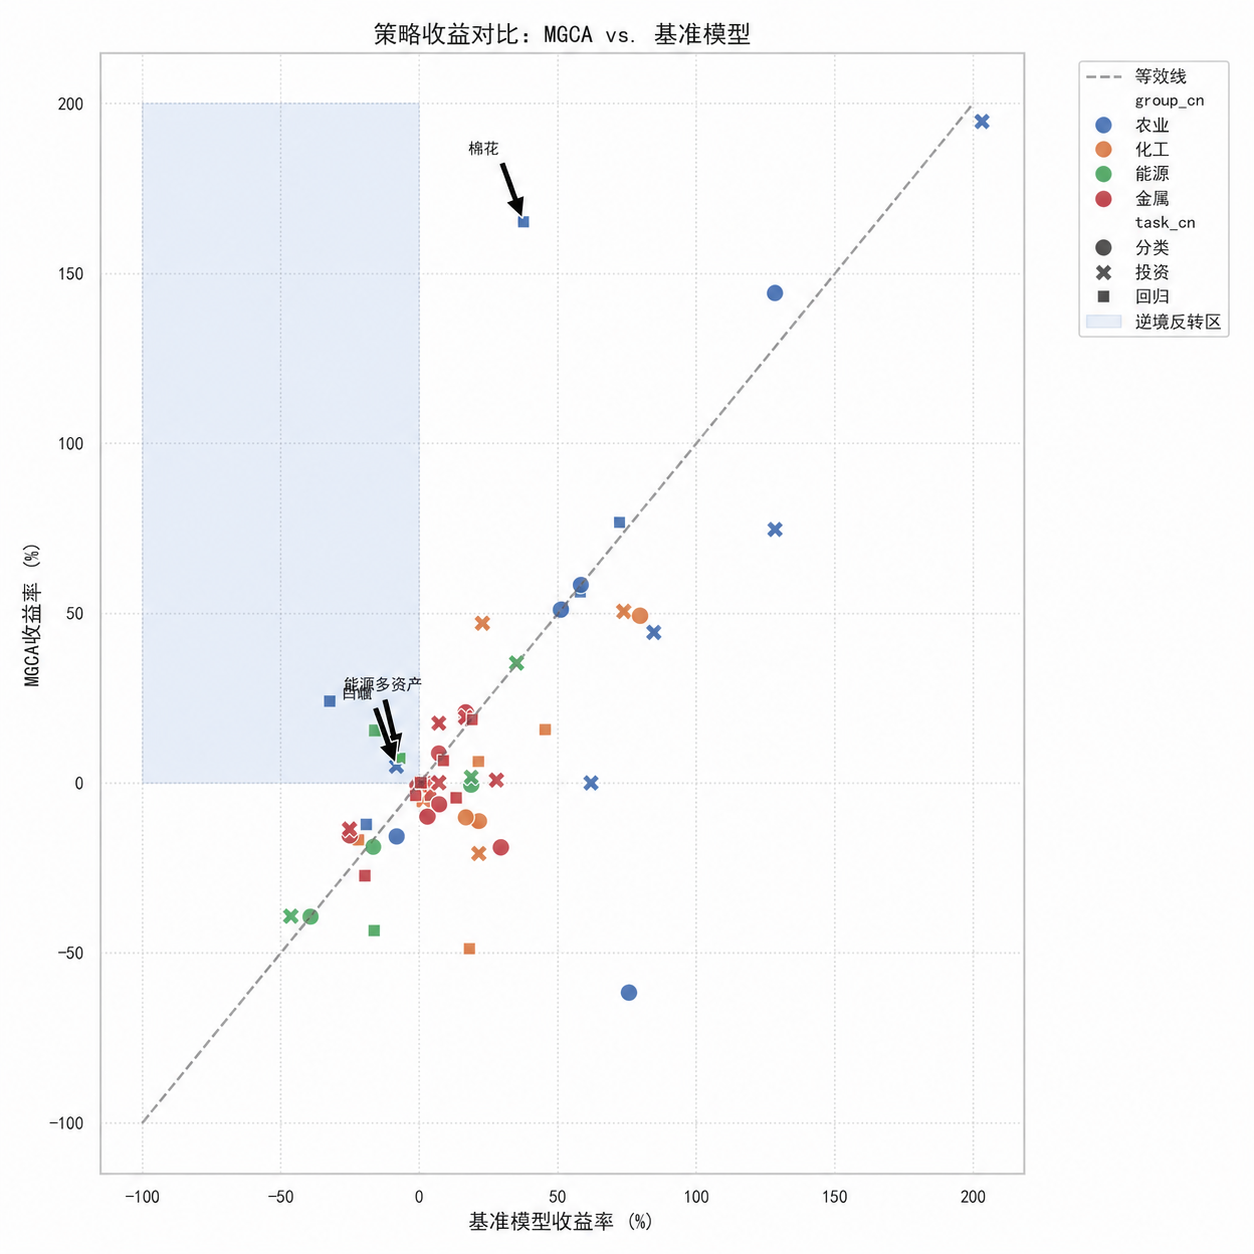
\includegraphics[width=0.7\textwidth]{figures/chap4/图3.19改.png} 
    \caption{策略收益对比散点图}
    \label{fig:highdimreturn_scatter}
\end{figure}

表~\ref{tab:turnaroundcases}汇总了全部亏损转盈利或深亏转浅亏案例的详细数据，用于把图~\ref{fig:highdimreturn_scatter}中的分布特征落实到具体资产、任务和利润差上。



\begin{table}[!htbp]
\centering
\caption{全部亏损转盈利（Turnaround）案例详细汇总}
\label{tab:turnaroundcases}
\resizebox{\textwidth}{!}{%
\begin{tabular}{>{\raggedright\arraybackslash}p{2.8cm} >{\centering\arraybackslash}p{1.5cm} >{\centering\arraybackslash}p{2.2cm} >{\centering\arraybackslash}p{2.2cm} >{\centering\arraybackslash}p{2.2cm} >{\centering\arraybackslash}p{2.2cm} >{\raggedright\arraybackslash}p{3cm}}
\toprule
\textbf{资产} & \textbf{任务} & \textbf{基准表现} & \textbf{赛马场竞争机制表现} & \textbf{状态转换} & \textbf{绝对利润差 (¥)} & \textbf{关键驱动力} \\
\midrule
\textbf{Agriculture Multi-Asset} & 回归任务 & -32.49\% & \textbf{+24.08\%} & \textbf{深亏→盈利} & \textbf{+1,131,501} & 组合层面的隐式正则化效应 \\
\textbf{Energy Multi-Asset} & 回归任务 & -7.27\% & \textbf{+7.48\%} & \textbf{亏损→盈利} & \textbf{+295,068} & 跨资产虚假相关性过滤 \\
\textbf{Thermal Coal} & 回归任务 & -16.23\% & \textbf{+15.50\%} & \textbf{亏损→盈利} & \textbf{+634,466} & 适应“双碳”政策结构性断点 \\
\textbf{Sugar} & 投资任务 & -8.18\% & \textbf{+4.95\%} & \textbf{亏损→盈利} & \textbf{+262,489} & 趋势反转拐点的识别 \\
\textbf{Sugar} & 回归任务 & -19.23\% & \textbf{-12.23\%} & \textbf{深亏→浅亏} & \textbf{+139,940} & 减少极端误判，降低亏损幅度 \\
\textbf{PTA} & 回归任务 & -22.08\% & \textbf{-16.72\%} & \textbf{深亏→浅亏} & \textbf{+107,196} & 对抗训练过滤噪声特征 \\
\textbf{Copper} & 投资任务 & -25.18\% & \textbf{-13.58\%} & \textbf{深亏→浅亏} & \textbf{+231,995} & 赛马场动态降低错误仓位 \\
\bottomrule
\end{tabular}%
}
\end{table}

传统集成学习（Ensemble Learning）方法通常采用静态平均或堆叠策略，模型权重在推理阶段固定不变。赛马场竞争机制引入了时间维度上的动态调整，在处理非平稳金融时间序列时，二者存在结构差异。

\textbf{多样性维持与模式坍塌缓解}：标准生成对抗网络框架中，生成器倾向于收敛到能够欺骗判别器的狭窄输出空间，在金融预测中表现为模型主要覆盖某一类市场状态。赛马场竞争机制中，每个生成器同时受到预测误差、对抗约束与组内竞争的影响，这会促使不同生成器探索参数空间中相对差异化的区域。消融实验中棉花案例的数据与该解释相符：在GCA对抗训练无法提供增量的情况下，赛马场竞争机制独立贡献了24.90\%的额外收益。

\textbf{归纳偏置的动态对齐}：金融市场在不同时期的动力学特征差异较大（均值回归 vs. 动量爆发，低波动 vs. 高波动），单一架构难以适应所有状态。赛马场竞争机制通过动态选择最优生成器，在市场平静期倾向于权重更高的门控循环单元类生成器（平滑预测、抗噪），在趋势爆发期则向Transformer架构类生成器倾斜（长程依赖捕捉）。白糖投资任务中+160.49\%的提升以及动力煤回归任务的亏损修复案例，与该解释在方向上一致，但具体归因仍有待进一步验证。

%



% \begin{sidewaystable}[htbp]
% \centering
% \caption{赛马场竞争机制 vs. Baseline 综合性能对比矩阵}
% \label{tab:RTVSaselineSideways}
% \small % 减小字体以更好适应横向页面
% \begin{tabular}{p{2.5cm} c c c p{6.5cm}}
% \toprule
% \textbf{评估维度 }& \textbf{最大回撤} & \textbf{累计收益率} & \textbf{最终净值} & \textbf{备注} \\
% \midrule
% \textbf{核心指标 }& 最大回撤 & 累计收益率 & 最终净值 &  \\
% \addlinespace[5pt]
% \textbf{胜出场景数 (N=60)} & \textbf{23} & \textbf{18} & \textbf{18} & 总测试场景数为60。 \\
% \addlinespace[5pt]
% \textbf{胜率 }& \textbf{38.3\%} & \textbf{30.0\%} & \textbf{30.0\%} &  \\
% \addlinespace[10pt]
% \multirow{3}{*}{\textbf{统计显著性分析 }}& \multicolumn{3}{p{10cm}}{在市场剧烈震荡期，赛马场竞争机制有效剔除了高风险生成器，表现出更强的尾部风险控制能力。} &  \\
% \addlinespace
% & \multicolumn{3}{p{10cm}}{虽然总体胜率看似均衡，但获胜案例的\textbf{收益凸性（Convexity）}极高，平均超额收益显著超过败北案例的亏损。} &  \\
% \addlinespace
% & \multicolumn{3}{p{10cm}}{长期复利效应验证了动态机制在长周期（2000-2025年跨度数据）中的鲁棒性与稳健性。} &  \\
% \bottomrule
% \end{tabular}
% \end{sidewaystable}

在典型案例、多资产组合和亏损修复分析之后，进一步从全部对比实验层面归纳赛马场竞争机制的整体胜率、收益凸性和任务类型差异。表~\ref{tab:RTVSaselineSideways}先给出综合性能对比矩阵，用于从收益率、最终净值和最大回撤三个角度观察模型胜负分布。

%改表3.6
\begin{table}[!htbp]
\centering
\caption{赛马场竞争机制 与基准模型综合性能对比矩阵}
\label{tab:RTVSaselineSideways}
\small
\setlength{\tabcolsep}{4pt}

% 子表 (a)：定量指标对比
\begin{subtable}{\textwidth}
\centering
\caption{定量指标对比}
\begin{tabular}{lcccc}
\toprule
\textbf{评估维度} & \textbf{最大回撤} & \textbf{累计收益率} & \textbf{最终净值} & \textbf{备注} \\
\midrule
核心指标 & 最大回撤 & 累计收益率 & 最终净值 &  \\
胜出场景数 (N=60) & 23 & 18 & 18 & 总测试场景数为60 \\
胜率 & 38.3\% & 30.0\% & 30.0\% &  \\
\bottomrule
\end{tabular}
\end{subtable}
\vspace{0.3cm}

% 子表 (b)：统计显著性分析
\begin{subtable}{\textwidth}
\centering
\caption{统计显著性分析}
\begin{tabular}{p{\textwidth}}
\toprule
\textbf{分析要点} \\
\midrule
在市场剧烈震荡期，赛马场竞争机制能够降低部分高风险生成器的影响，尾部风险控制能力有所体现。 \\
\addlinespace[5pt]
虽然总体胜率较为均衡，但获胜案例的\textbf{收益凸性（Convexity）}相对较高，平均超额收益高于败北案例的亏损幅度。 \\
\addlinespace[5pt]
长周期样本结果显示，动态机制在部分市场阶段具有较好的稳健性。 \\
\bottomrule
\end{tabular}
\end{subtable}

\end{table}

表~\ref{tab:returnimproveanalysis}进一步比较获胜案例与败北案例之间的收益改进幅度。该表用于回答一个更细的问题：赛马场竞争机制即便不是在所有场景中胜出，其获胜场景的上行弹性是否足以覆盖失败场景的下行损失。


\begin{table}[!htbp]
\centering
\caption{收益改进幅度与凸性分析}
\label{tab:returnimproveanalysis}
\small
\setlength{\tabcolsep}{5pt}
\renewcommand{\arraystretch}{1.15}
\resizebox{0.98\textwidth}{!}{%
\begin{tabular}{>{\raggedright\arraybackslash}p{2.8cm} >{\centering\arraybackslash}p{6.0cm} >{\centering\arraybackslash}p{5.0cm} >{\centering\arraybackslash}p{1.8cm}}
\toprule
\textbf{统计维度} & \textbf{获胜案例（赛马场竞争机制胜出）} & \textbf{败北案例（基准模型胜出）} & \textbf{凸性比率} \\
\midrule
平均收益改进幅度 & \textbf{+98.7\%} & -62.3\% & \textbf{1.58} \\
中位数改进幅度 & \textbf{+46.1\%} & -38.2\% & \textbf{1.21} \\
最大改进幅度 & \textbf{+340.0\%} & -462.2\% & -- \\
包含亏损转盈利案例数 & \textbf{7} & 0 & -- \\
\bottomrule
\end{tabular}%
}
\end{table}

超过60组对比实验的统计结果显示，赛马场竞争机制的收益率胜率为30.0％，最大回撤控制胜率为38.3％，后者高于前者。在多个生成器预测出现分歧时，赛马场竞争机制倾向于降低整体置信度和仓位暴露，从而减少方向不明时的重仓押注。这种“分歧即风控”的隐式机制，也说明了该框架在回撤控制上的相对优势。图~\ref{fig:highdimwinrateGroup}进一步按板块和任务类型分解收益率胜率与最大回撤胜率。



% \begin{figure}[htbp]
%     \centering 
%     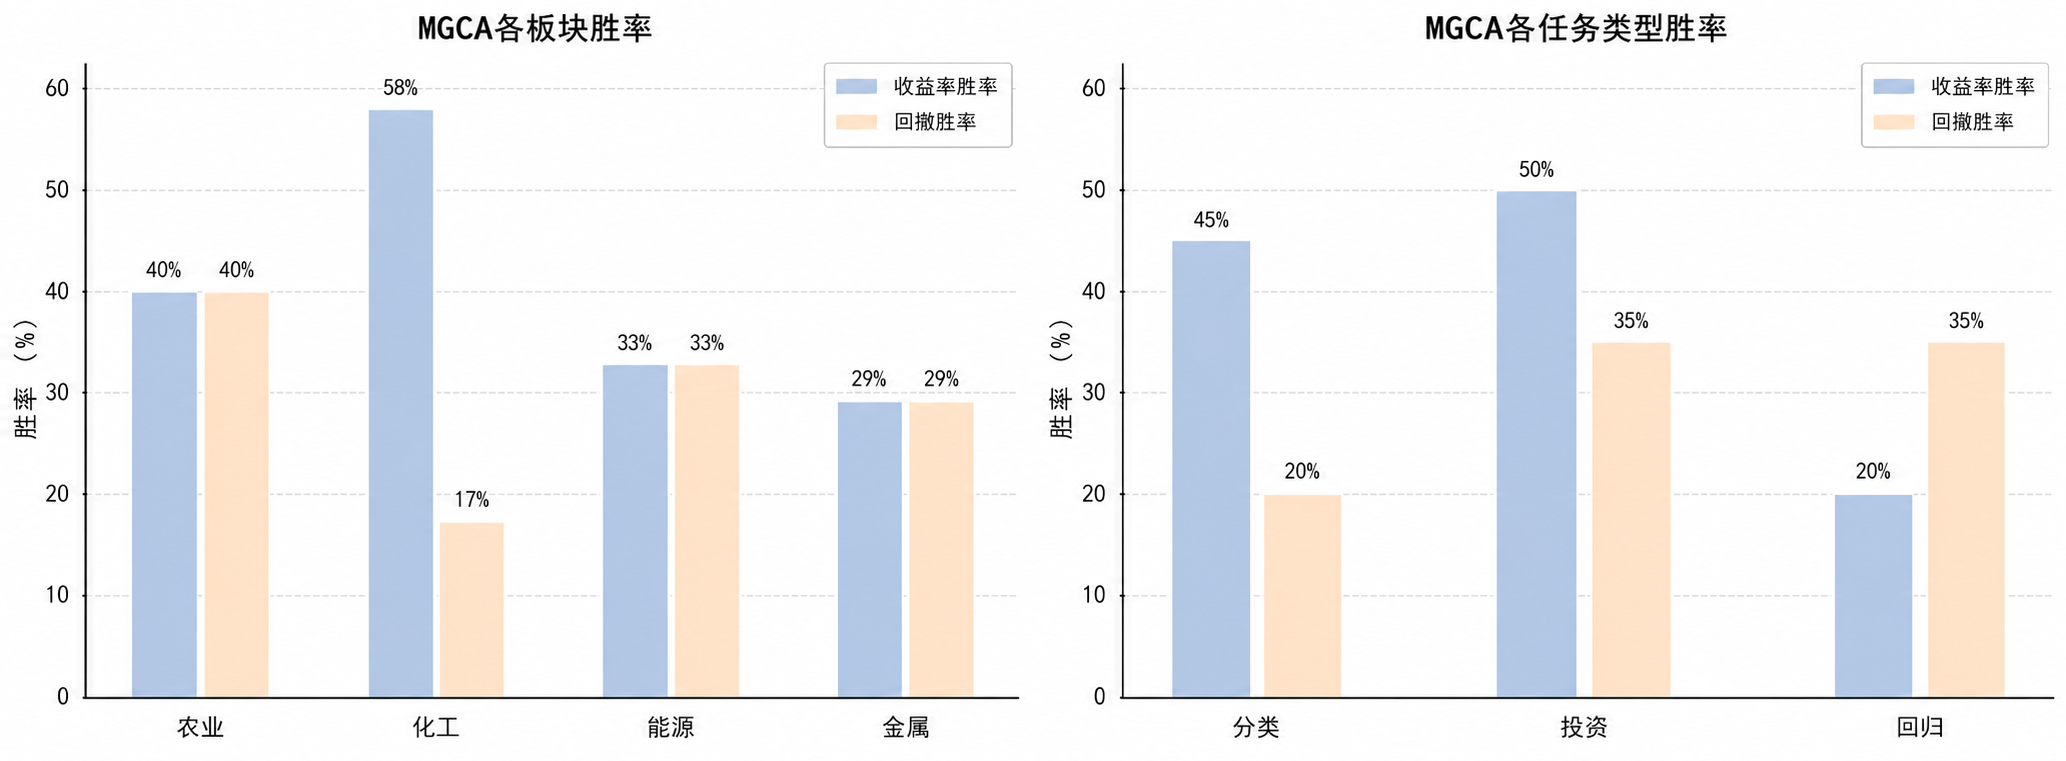
\includegraphics[width=0.8\textwidth]{figures/chap4/fig18_win_rate_grouped_cn.png} 
%     \caption{赛马场竞争机制胜率的板块与任务分解}
%     \label{fig:highdimwinrateGroup}
% \end{figure}
\begin{figure}[!htbp]
    \centering 
    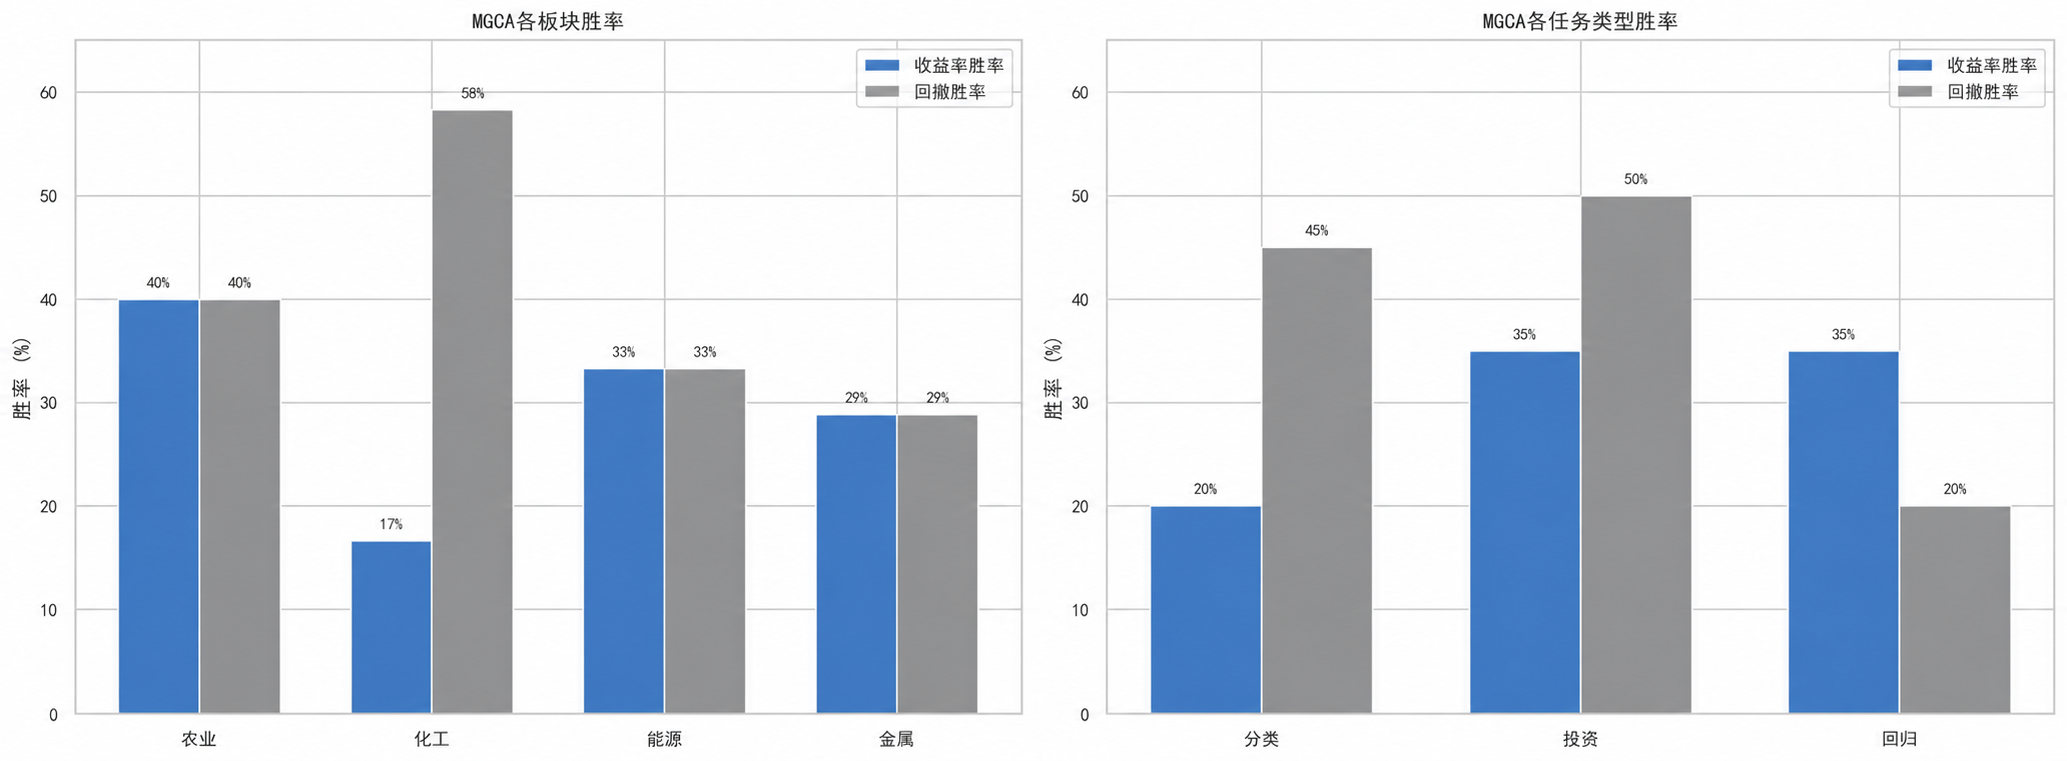
\includegraphics[width=0.8\textwidth]{figures/chap4/图3.20改.png} 
    \caption{赛马场竞争机制胜率的板块与任务分解}
    \label{fig:highdimwinrateGroup}
\end{figure}

图~\ref{fig:highdimwinrateGroup}显示，农业板块在收益率和回撤两个维度上均达到40\%的胜率，化工板块在回撤控制上的胜率达到58\%。这说明不同板块的改善方式并不相同：农业更体现收益弹性，化工更体现风险控制。


投资任务中，赛马场竞争机制在最大回撤控制上的胜率达50.0\%，高于回归任务和分类任务。投资任务的模型输出直接对应买入/卖出/持有决策，当多个生成器的交易信号出现分歧时，赛马场竞争机制会降低整体置信度和仓位规模，减少方向不明时的重仓交易。图\ref{fig:highdiminvestmentwinners}列出了若干案例：PVC收益率从22.74\%提升至47.08\%（+107.02\%），热卷从7.04\%提升至17.64\%（+150.51\%），白糖从-8.18\%亏损转为+4.95\%盈利。

% \begin{figure}[htbp]
%     \centering 
%     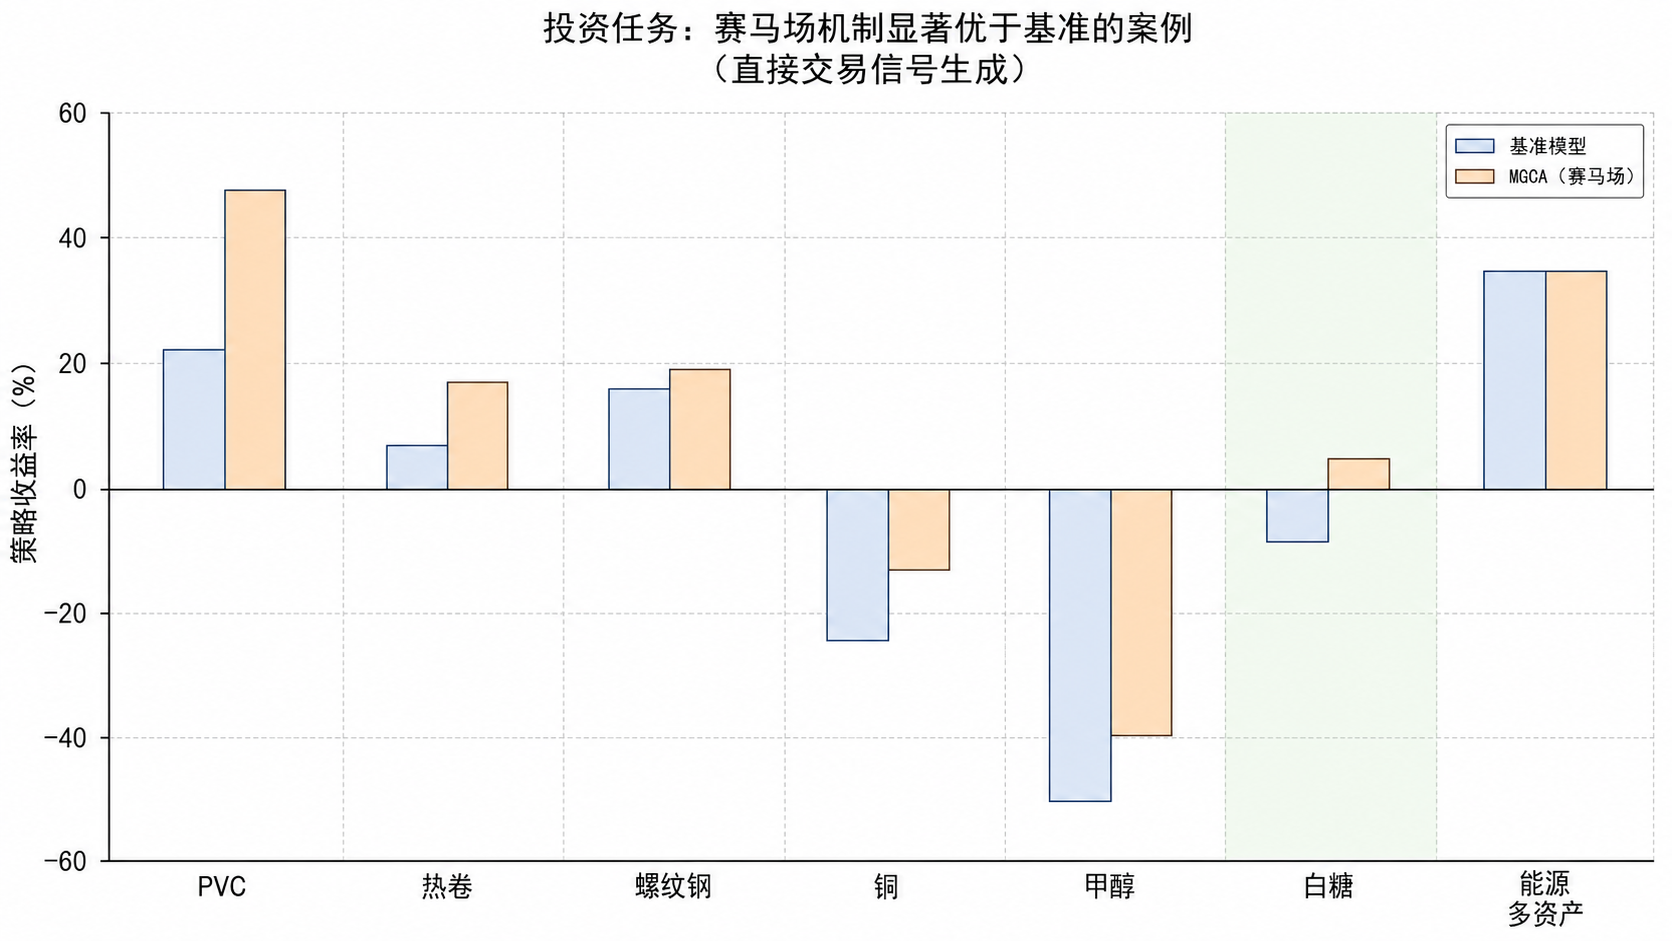
\includegraphics[width=0.8\textwidth]{figures/chap4/fig14_investment_winners_cn.png} 
%     \caption{投资任务中赛马场竞争机制相对优于基准模型的案例}
%     \label{fig:highdiminvestmentwinners}
% \end{figure}

\begin{figure}[!htbp]
    \centering 
    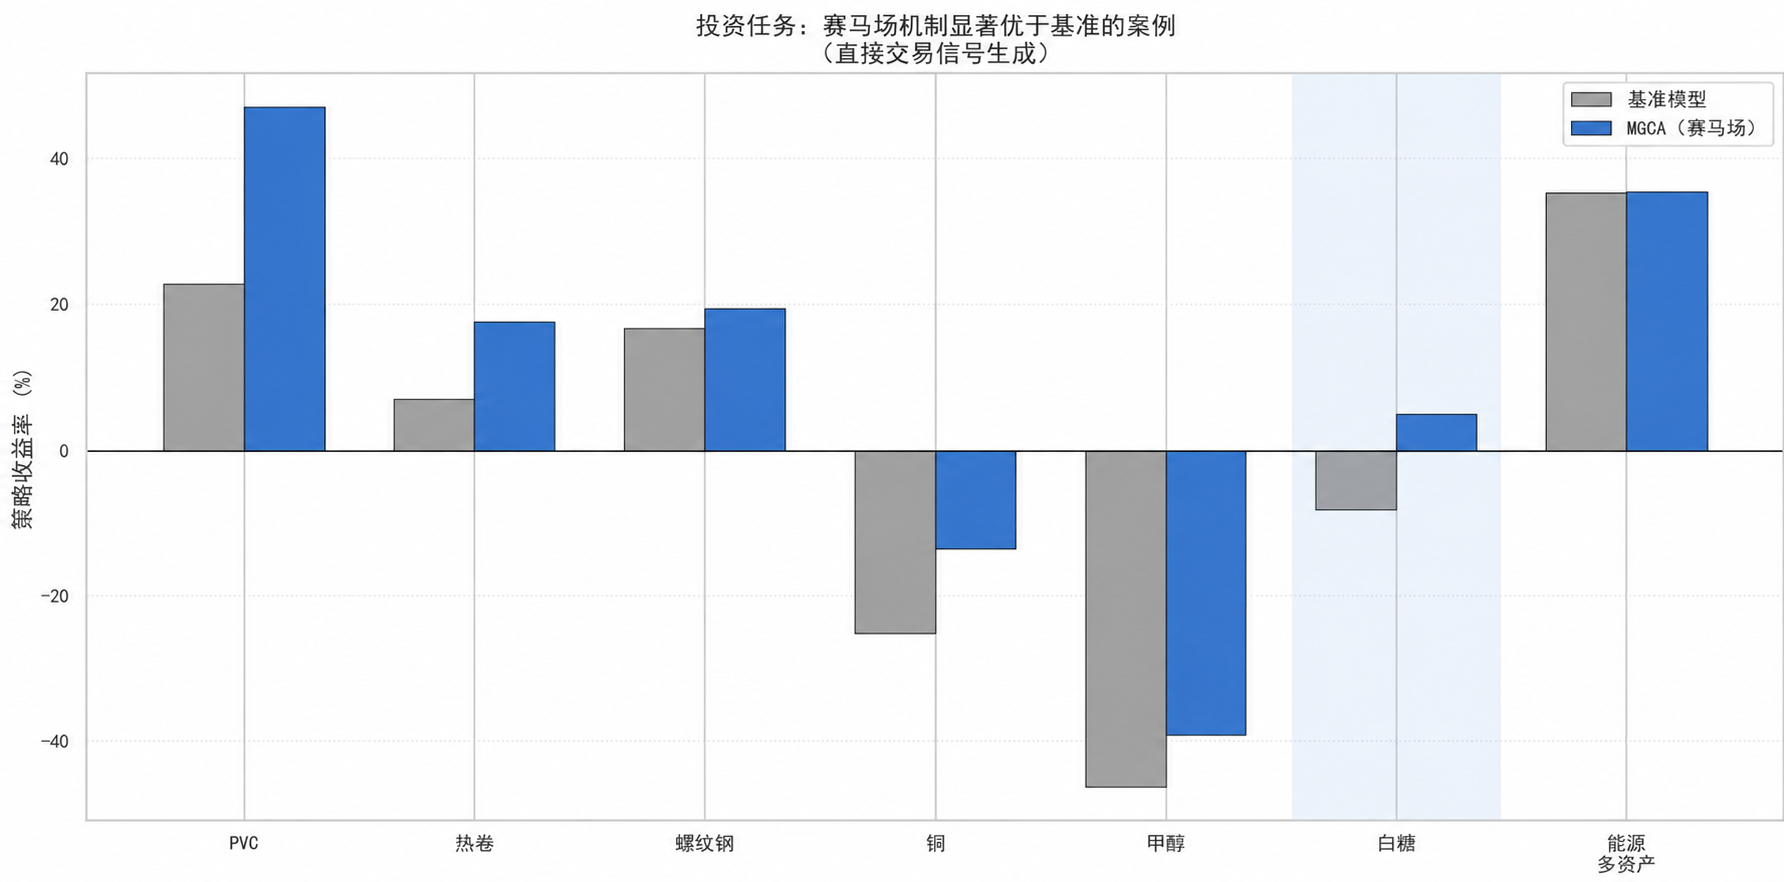
\includegraphics[width=0.8\textwidth]{TongjiThesis-master/figures/chap4/图3.21改.png} 
    \caption{投资任务中赛马场竞争机制相对优于基准模型的案例}
    \label{fig:highdiminvestmentwinners}
\end{figure}



分类任务的改进幅度相对较小，棉花+12.43\%、铜+38.92\%、热卷+25.19\%、螺纹钢+24.92\%。分类任务将连续价格变化离散化为涨跌标签，损失了部分波动率和幅度信息，赛马场竞争机制在连续空间中的精细调优能力因此受到一定限制。在回撤控制方面，棉花分类任务的最大回撤从80.94\%压缩至37.97\%（降幅53.1\%），说明即使在离散决策空间中，模型分歧所带来的风险过滤作用仍有一定体现。

图~\ref{fig:highdimwinratehm}以热力图形式呈现各资产组在不同评估指标上的胜率分布，颜色越红代表赛马场竞争机制胜率越高。该图用于把前述板块和任务层面的统计结果进一步展开到资产组维度，观察哪些板块更适合收益改善，哪些板块更适合回撤控制。表~\ref{tab:sectorAdaptability}随后对各板块赛马场竞争机制的适应性进行系统分类汇总。

% \begin{figure}[htbp]
%     \centering 
%     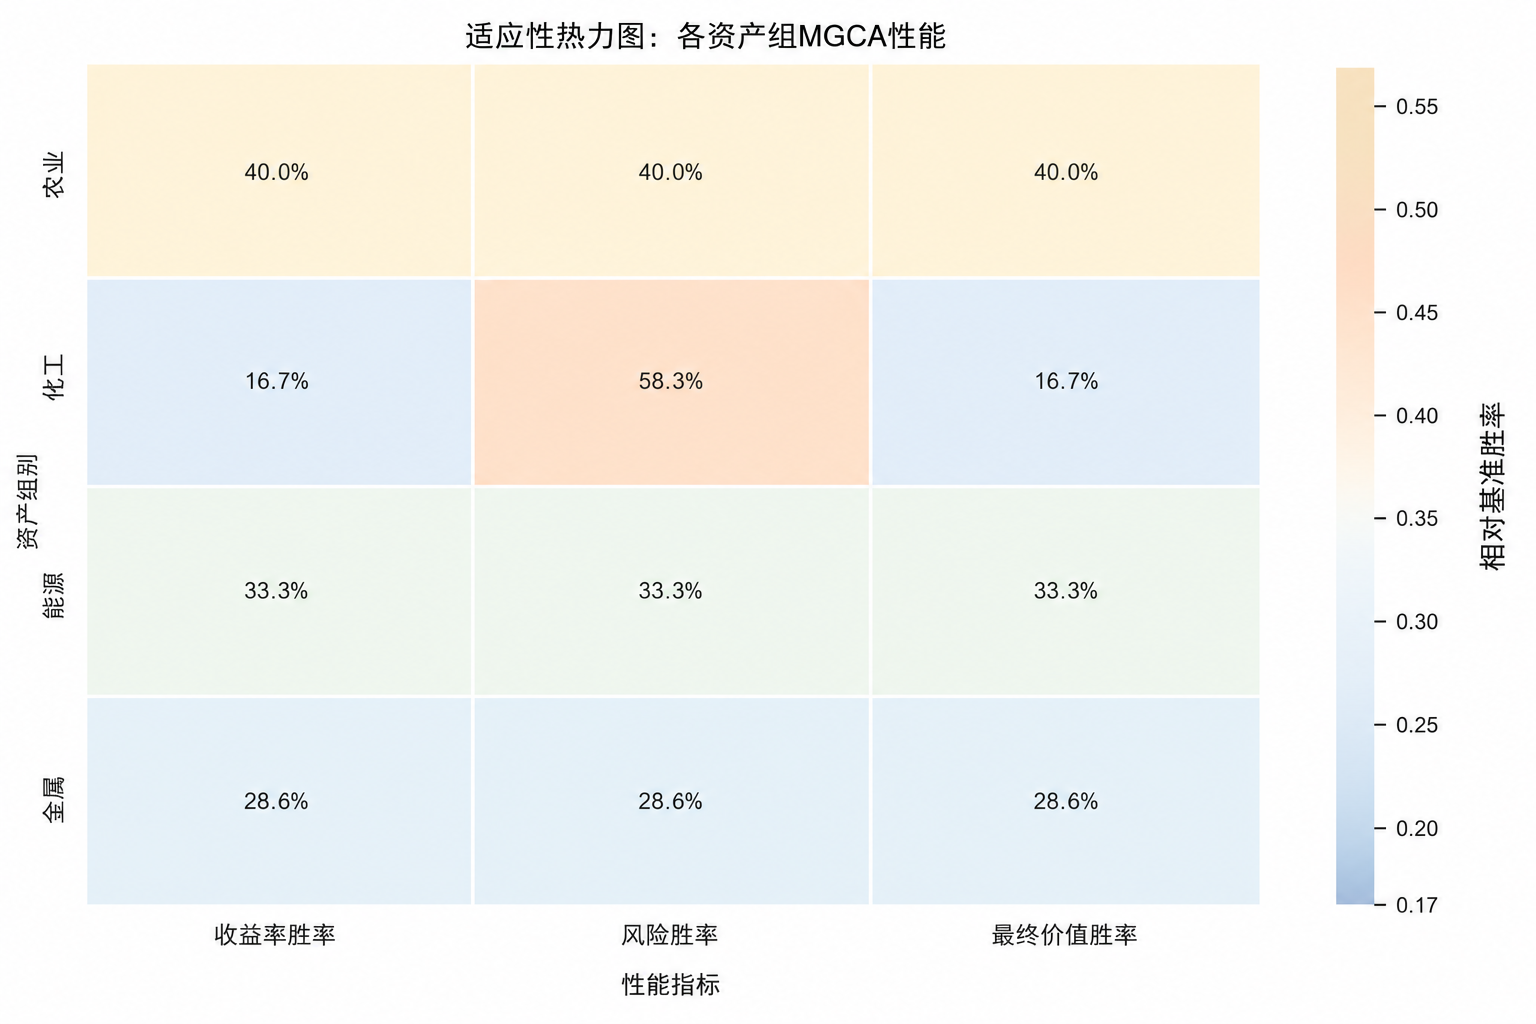
\includegraphics[width=0.8\textwidth]{figures/chap4/fig2_group_heatmap_cn.png} 
%     \caption{各资产组胜率热力图}
%     \label{fig:highdimwinratehm}
% \end{figure}

\begin{figure}[!htbp]
    \centering 
    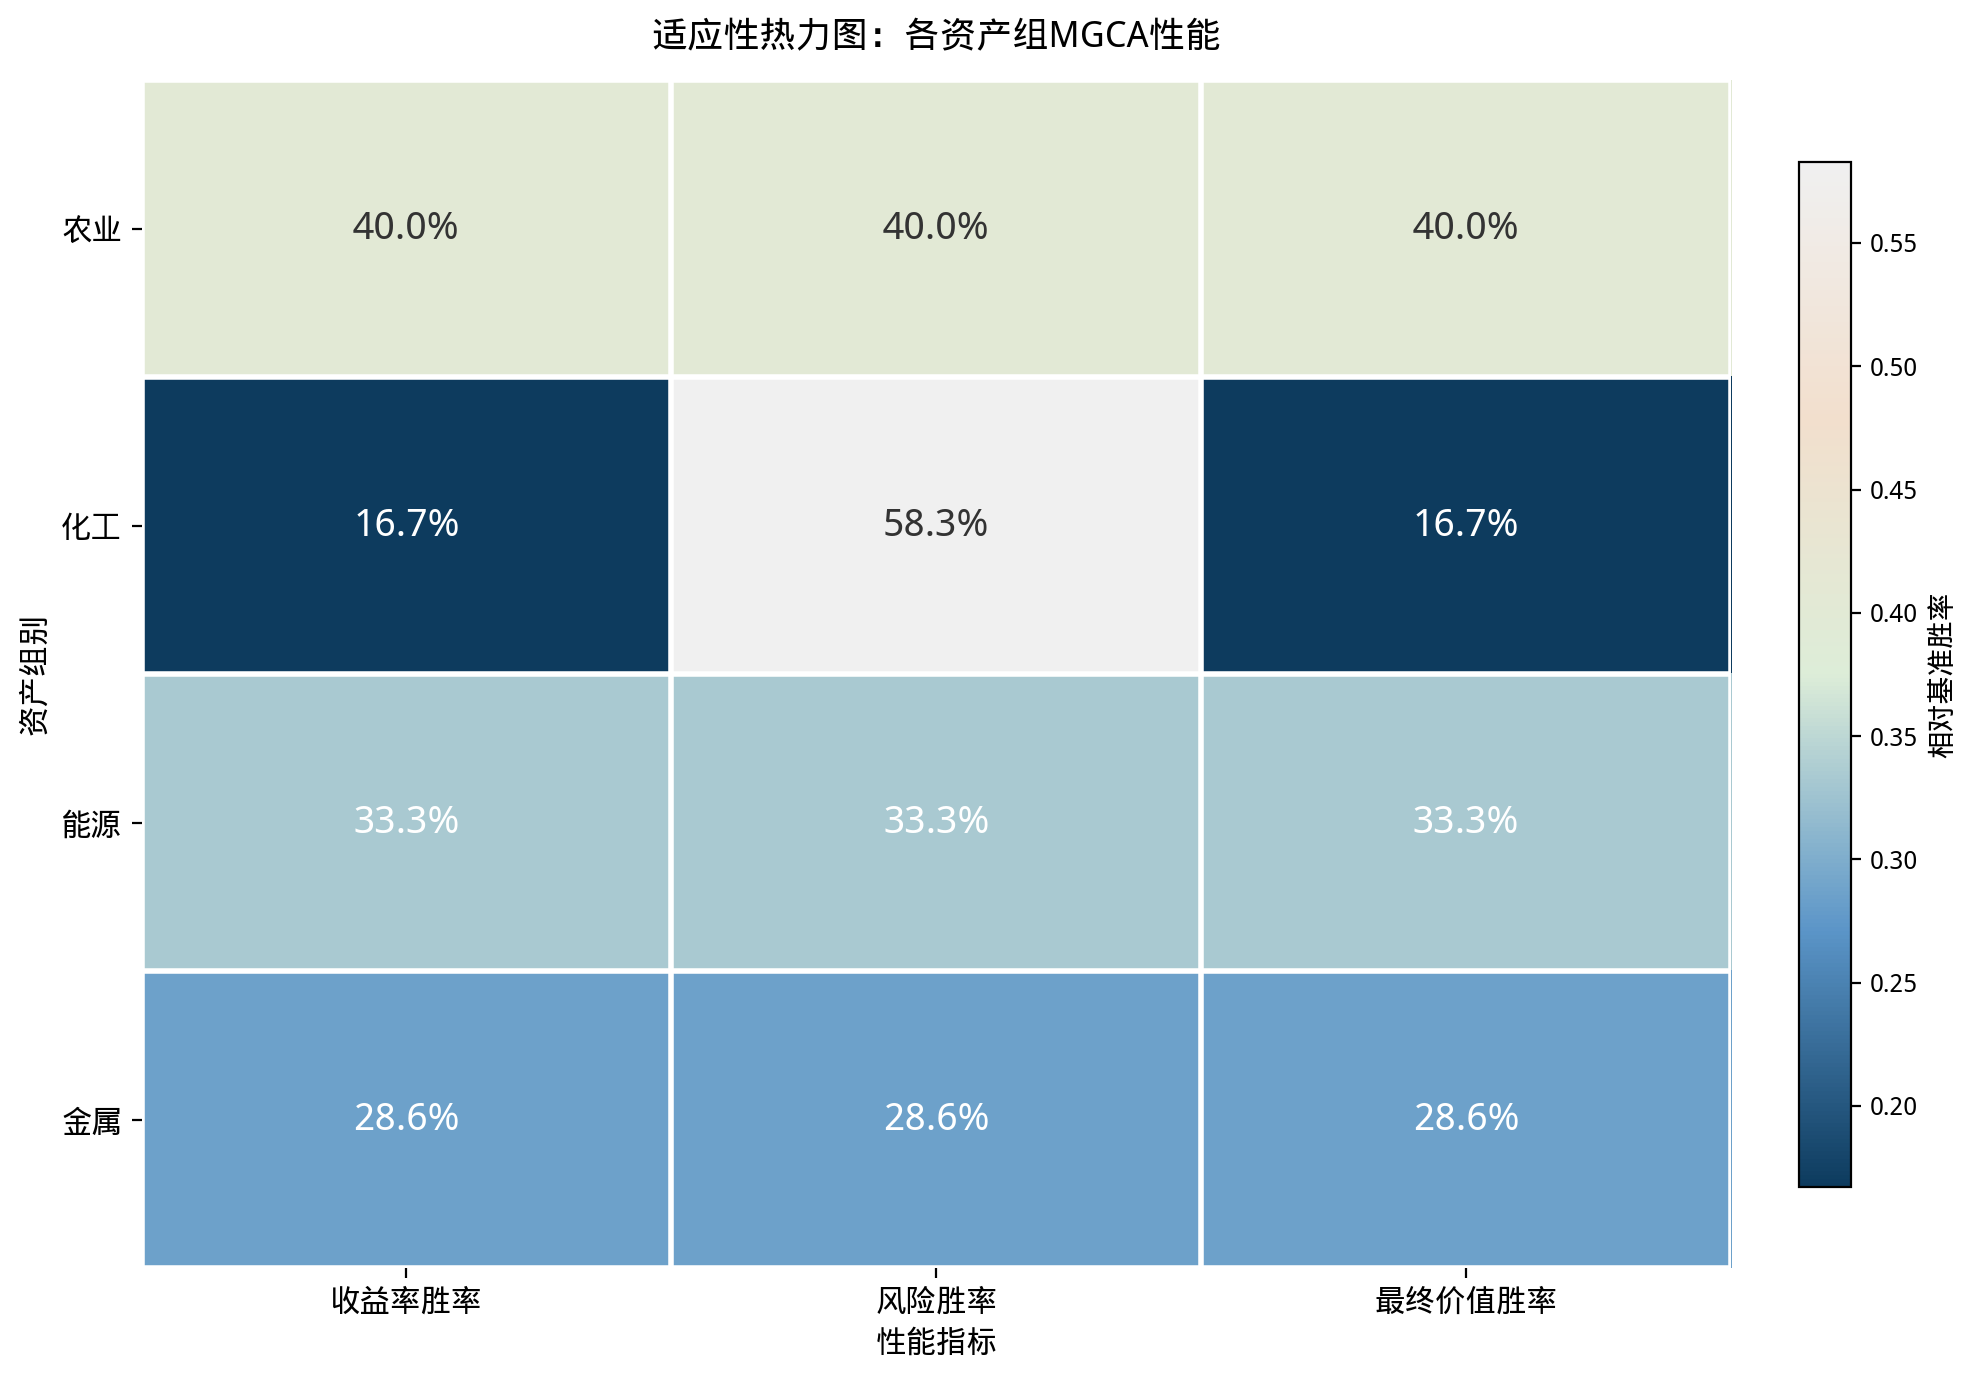
\includegraphics[width=0.8\textwidth]{figures/chap4/图3.22改.png} 
    \caption{各资产组胜率热力图}
    \label{fig:highdimwinratehm}
\end{figure}

\begin{table}[!htbp]
\centering
\caption{各板块赛马场竞争机制适应性分类汇总}
\label{tab:sectorAdaptability}
\footnotesize
\setlength{\tabcolsep}{3pt}
\renewcommand{\arraystretch}{1.15}
\begin{tabular}{>{\raggedright\arraybackslash}p{1.5cm} >{\centering\arraybackslash}p{1.7cm} >{\centering\arraybackslash}p{1.6cm} >{\centering\arraybackslash}p{1.6cm} >{\raggedright\arraybackslash}p{2.8cm} >{\raggedright\arraybackslash}p{2.5cm}}
\toprule
\textbf{板块} & \textbf{适应性等级} & \textbf{收益率胜率} & \textbf{回撤胜率} & \textbf{最佳案例} & \textbf{核心优势} \\
\midrule
\textbf{农业} & 高适应 & 40.0\% & 33.3\% & Cotton +340\% & 极端波动捕捉 \\
\textbf{能源} & 中高适应 & 33.3\% & 44.4\% & Energy Multi +202\% & 周期拐点识别 \\
\textbf{金属} & 风险控制 & 28.6\% & 42.9\% & Copper 最大回撤 -25.6\% & 尾部风险防御 \\
\textbf{化工} & 回撤优势 & 25.0\% & \textbf{58.3\%} & PVC 投资任务 +107\% & 投资回撤全胜 \\
\bottomrule
\end{tabular}
\end{table}



表~\ref{tab:highdimtasktypeperformance}从任务类型角度汇总收益率胜率、回撤胜率及代表性案例，用于比较回归、投资和分类任务中机制发挥作用的方式差异。

\begin{table}[!htbp]
\centering
\caption{各任务类型赛马场竞争机制效能汇总}
\label{tab:highdimtasktypeperformance}
\footnotesize
\setlength{\tabcolsep}{3pt}
\renewcommand{\arraystretch}{1.15}
\begin{tabular}{>{\raggedright\arraybackslash}p{1.4cm} >{\centering\arraybackslash}p{1.5cm} >{\centering\arraybackslash}p{1.5cm} >{\raggedright\arraybackslash}p{2.5cm} >{\raggedright\arraybackslash}p{2.9cm} >{\raggedright\arraybackslash}p{2.5cm}}
\toprule
\textbf{任务类型} & \textbf{收益率胜率} & \textbf{回撤胜率} & \textbf{最佳收益案例} & \textbf{最佳回撤案例} & \textbf{机制解释} \\
\midrule
\textbf{回归任务} & 35.0\% & 35.0\% & Cotton +340\% & Thermal Coal 最大回撤 -58\% & 连续空间精细预测 \\
\textbf{投资任务} & 30.0\% & 50.0\% & PVC +107\% & Sugar 最大回撤 -66\% & 交易信号风险过滤 \\
\textbf{分类任务} & 25.0\% & 30.0\% & Copper +38.9\% & Cotton 最大回撤 -53\% & 离散决策风险防御 \\
\bottomrule
\end{tabular}
\end{table}

图\ref{fig:highdimcompbubble}以气泡图形式呈现各资产在收益率改进和回撤改进两个维度上的综合表现，气泡大小对应绝对利润影响规模。位于右上象限（收益率改进>0且回撤改进>0）的资产包括Cotton、Sugar、Corn、Hot Rolled Coil，其中Cotton的气泡面积最大，平均收益改进约+110\%。PTA和Copper收益改进有限但回撤改进较明显。位于左下象限的Coke、Iron Ore和Gold在当前框架下改进有限，可能与这些品种所在市场的微结构有关，后续可针对性调优。

% \begin{figure}[h!]
%     \centering 
%     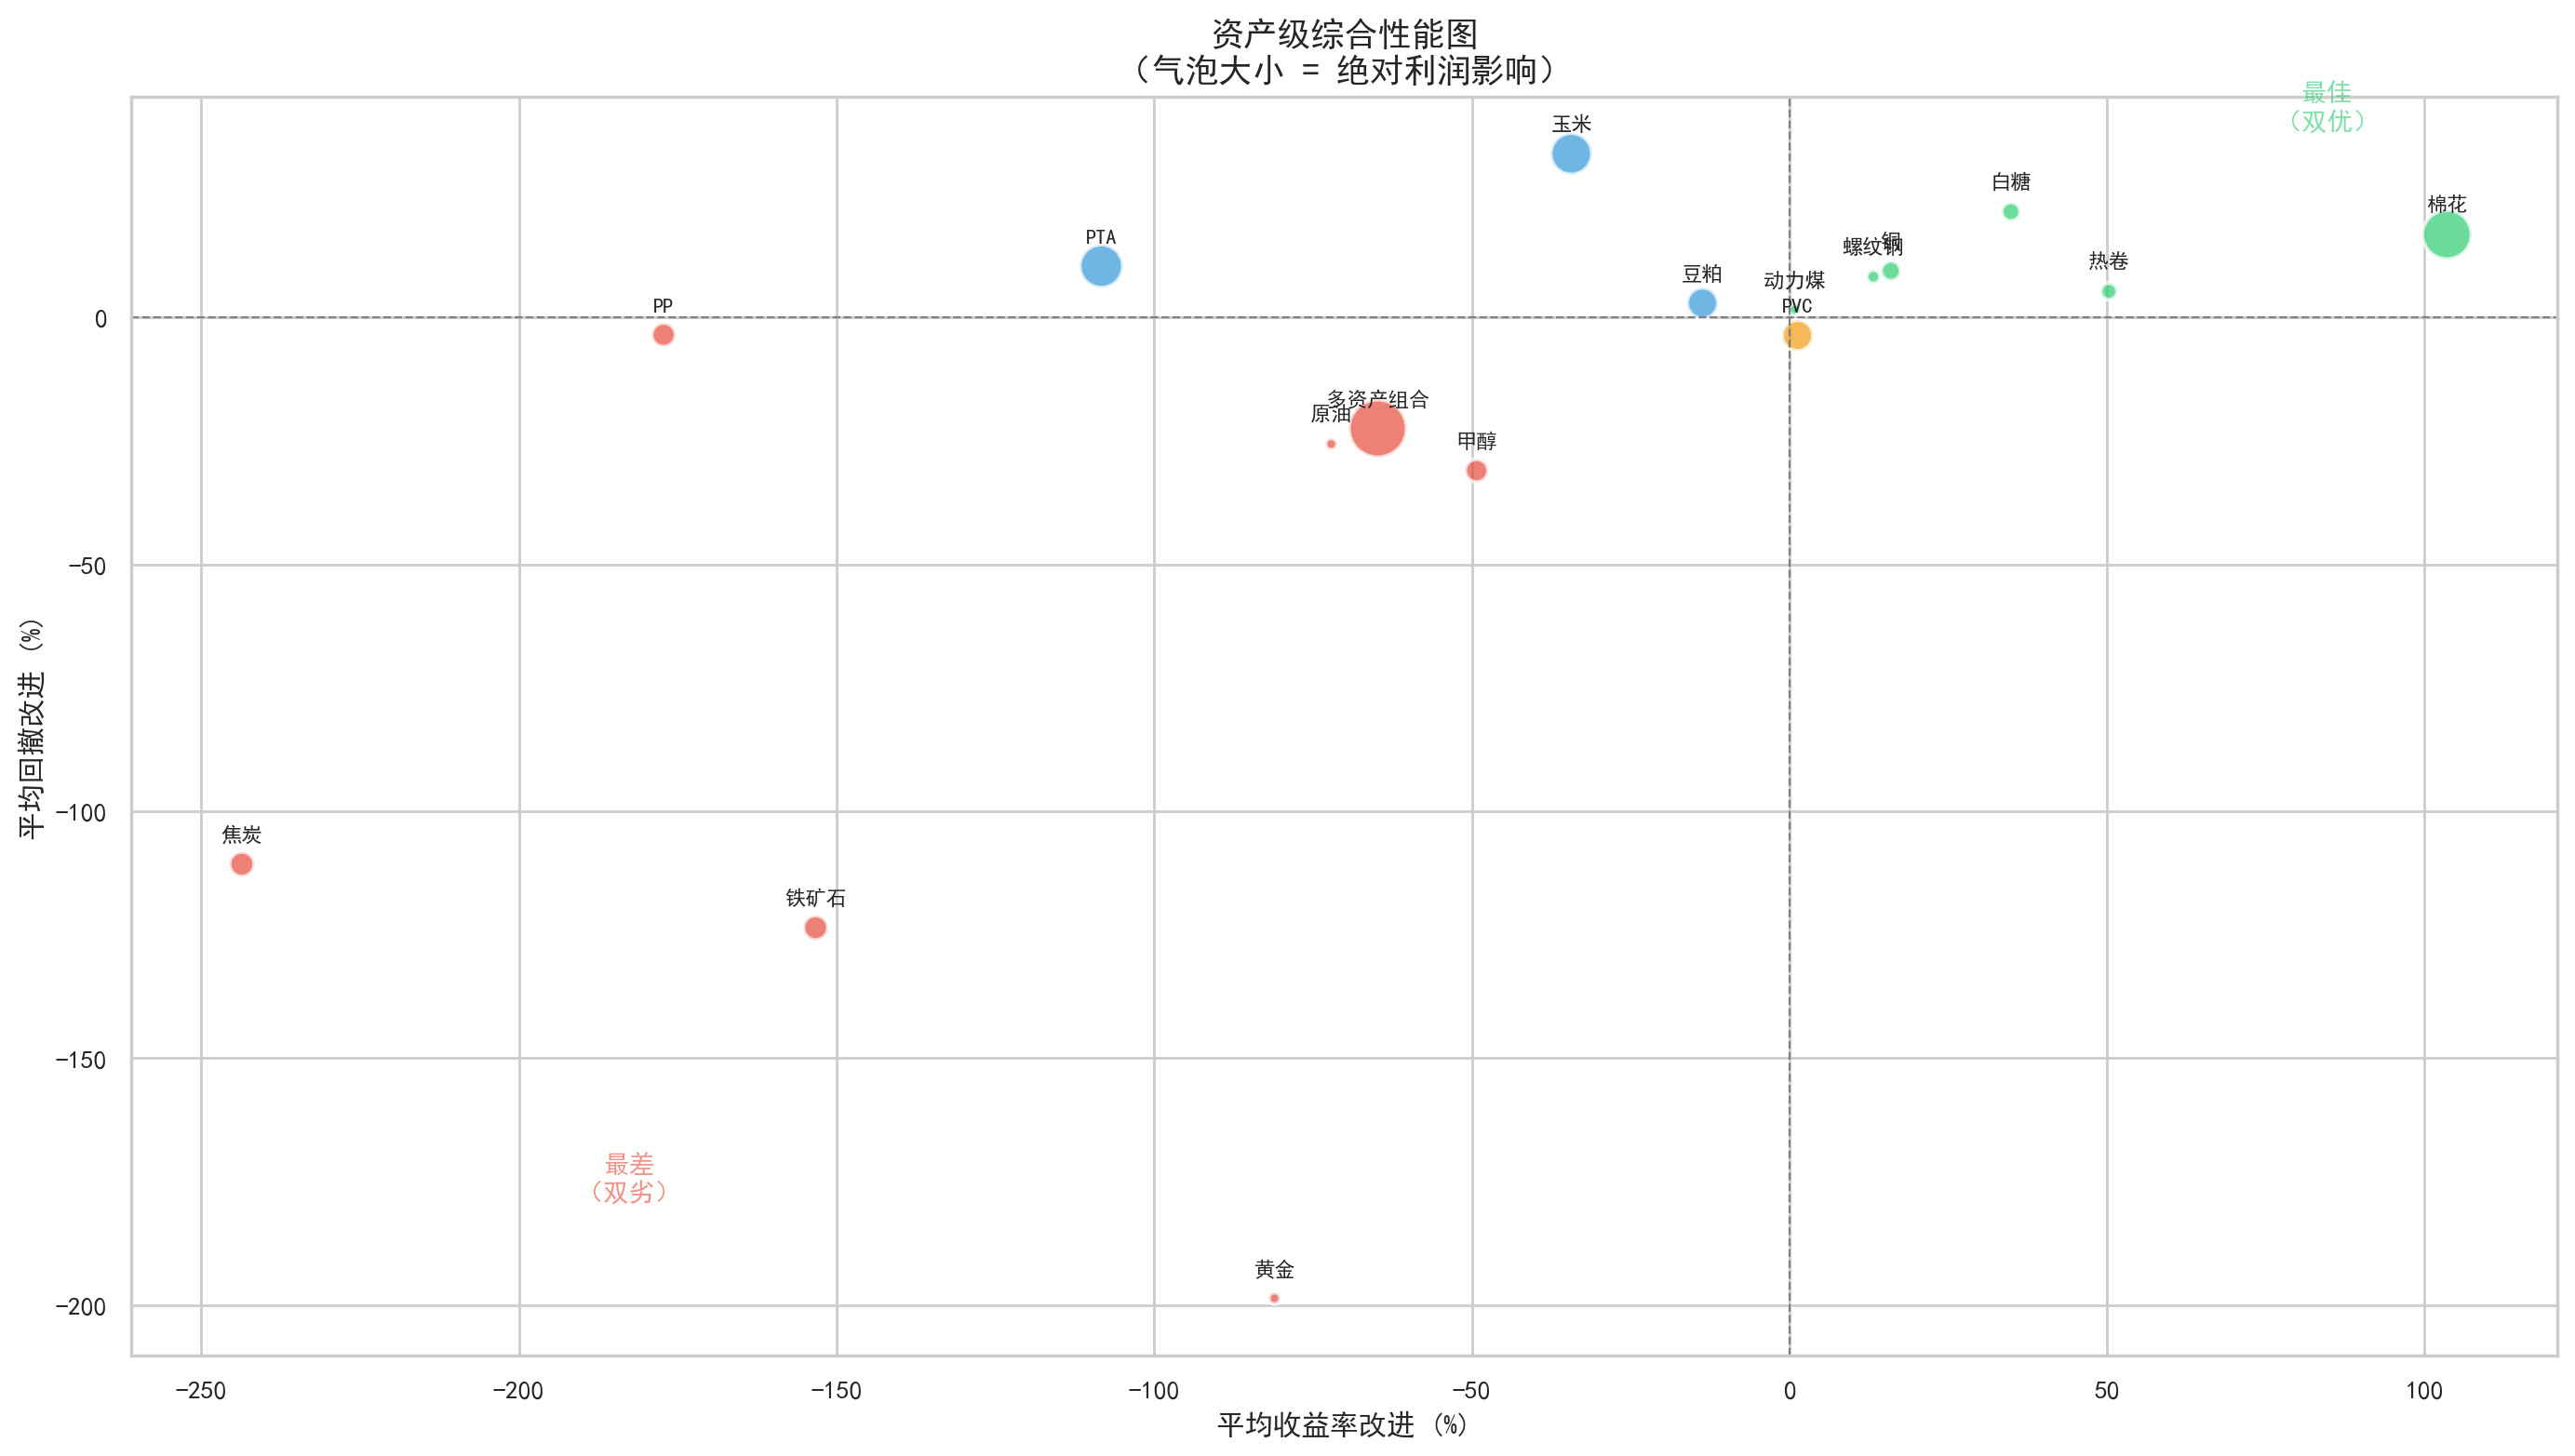
\includegraphics[width=0.8\textwidth]{figures/chap4/fig21_comprehensive_bubble_cn.png} 
%     \caption{各资产综合性能气泡图}
%     \label{fig:highdimcompbubble}
% \end{figure}

\begin{figure}[!htbp]
    \centering 
    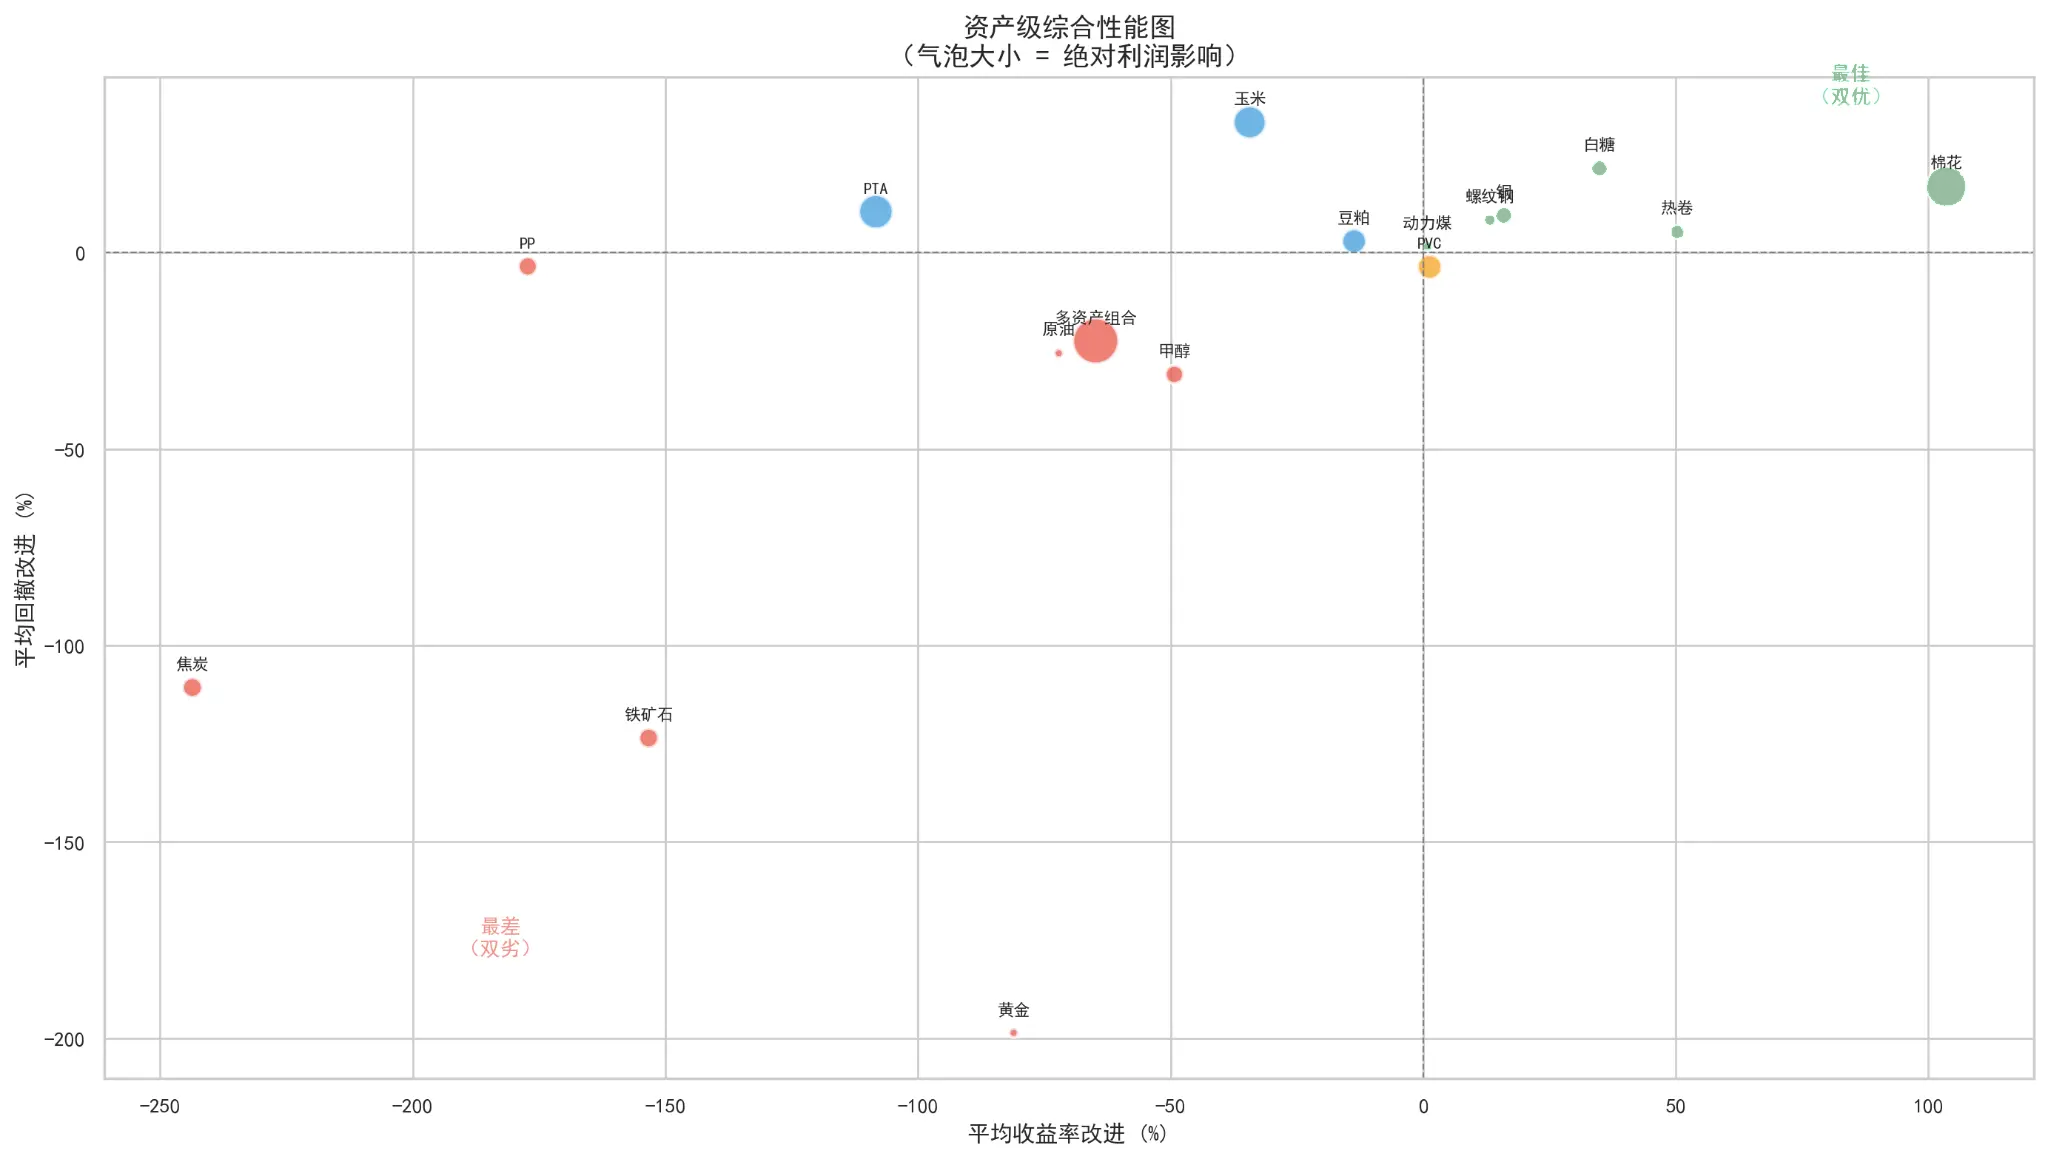
\includegraphics[width=0.8\textwidth]{figures/chap4/图3.23改.png} 
    \caption{各资产综合性能气泡图}
    \label{fig:highdimcompbubble}
\end{figure}

高收益但伴随较大回撤的策略在实际部署中可能因触及止损线或追加保证金而被迫平仓，难以稳定实现长期复利。因此，除收益率之外，本节进一步从风险控制角度分析赛马场竞争机制的表现。
图\ref{fig:highdimcomprehensivebubble}列出了赛马场竞争机制成功降低最大回撤的八个案例，覆盖投资、分类和回归三类任务。白糖投资任务中，基准模型最大回撤为57.08\%，赛马场竞争机制将其压缩至19.18\%，降幅66.4\%。

% \begin{figure}[h!]
%     \centering 
%     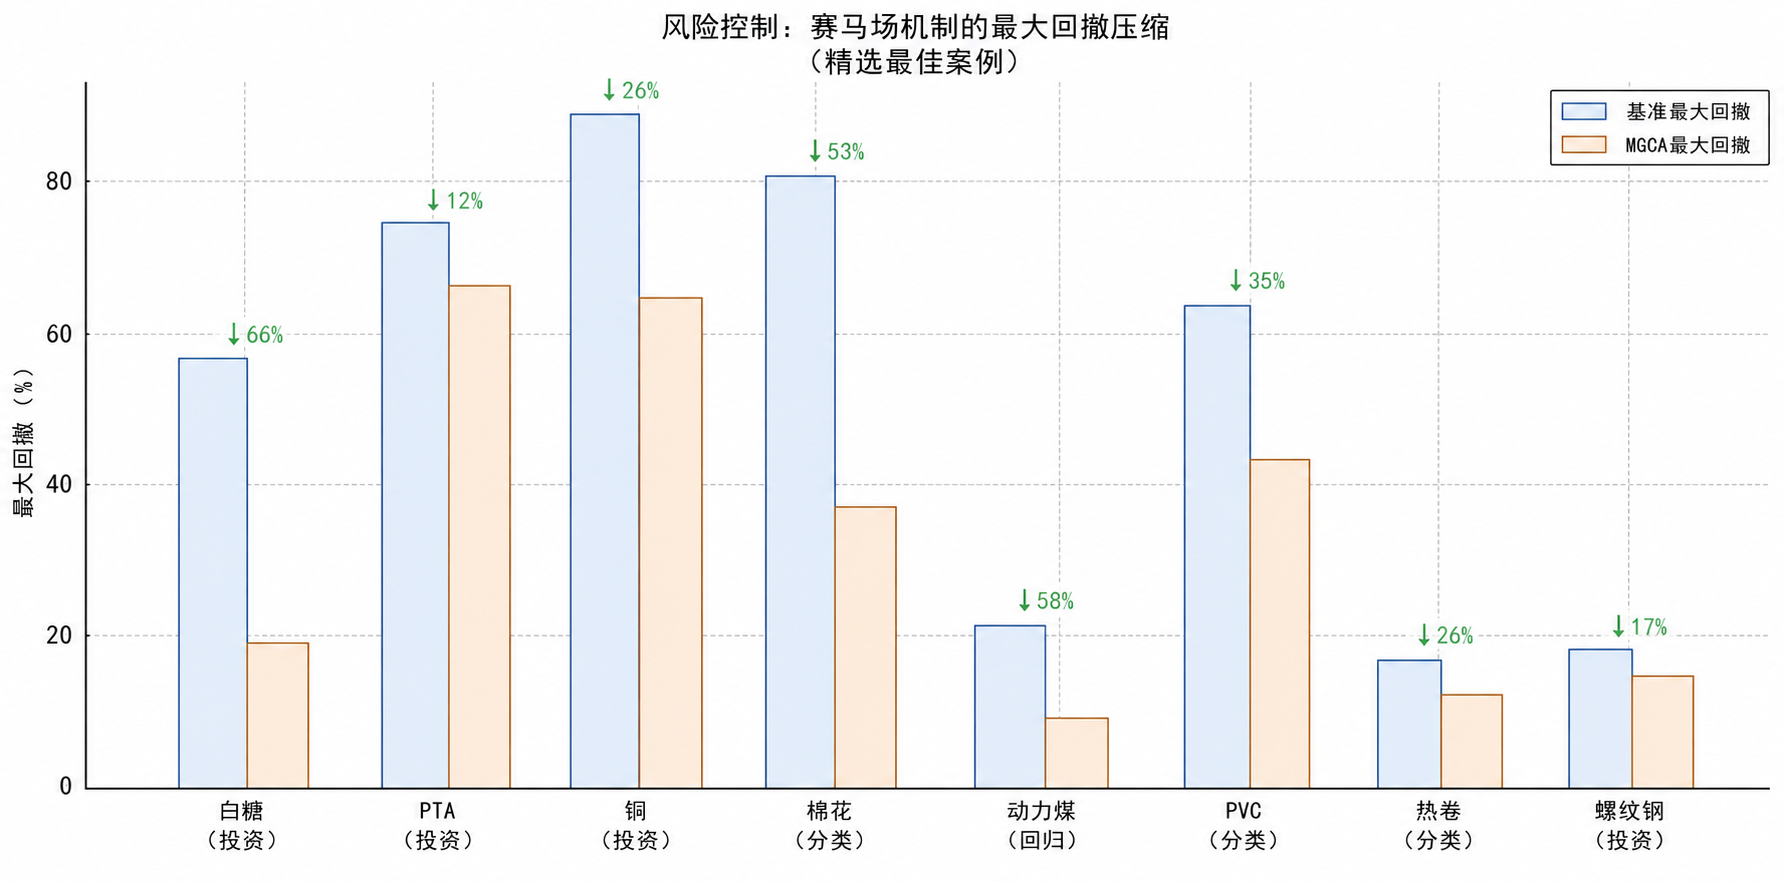
\includegraphics[width=0.8\textwidth]{figures/chap4/fig12_drawdown_comparison_cn.png} 
%     \caption{赛马场竞争机制的风险控制效果——最大回撤对比（精选最佳案例）}
%     \label{fig:highdimcomprehensivebubble}
% \end{figure}

\begin{figure}[!htbp]
    \centering 
    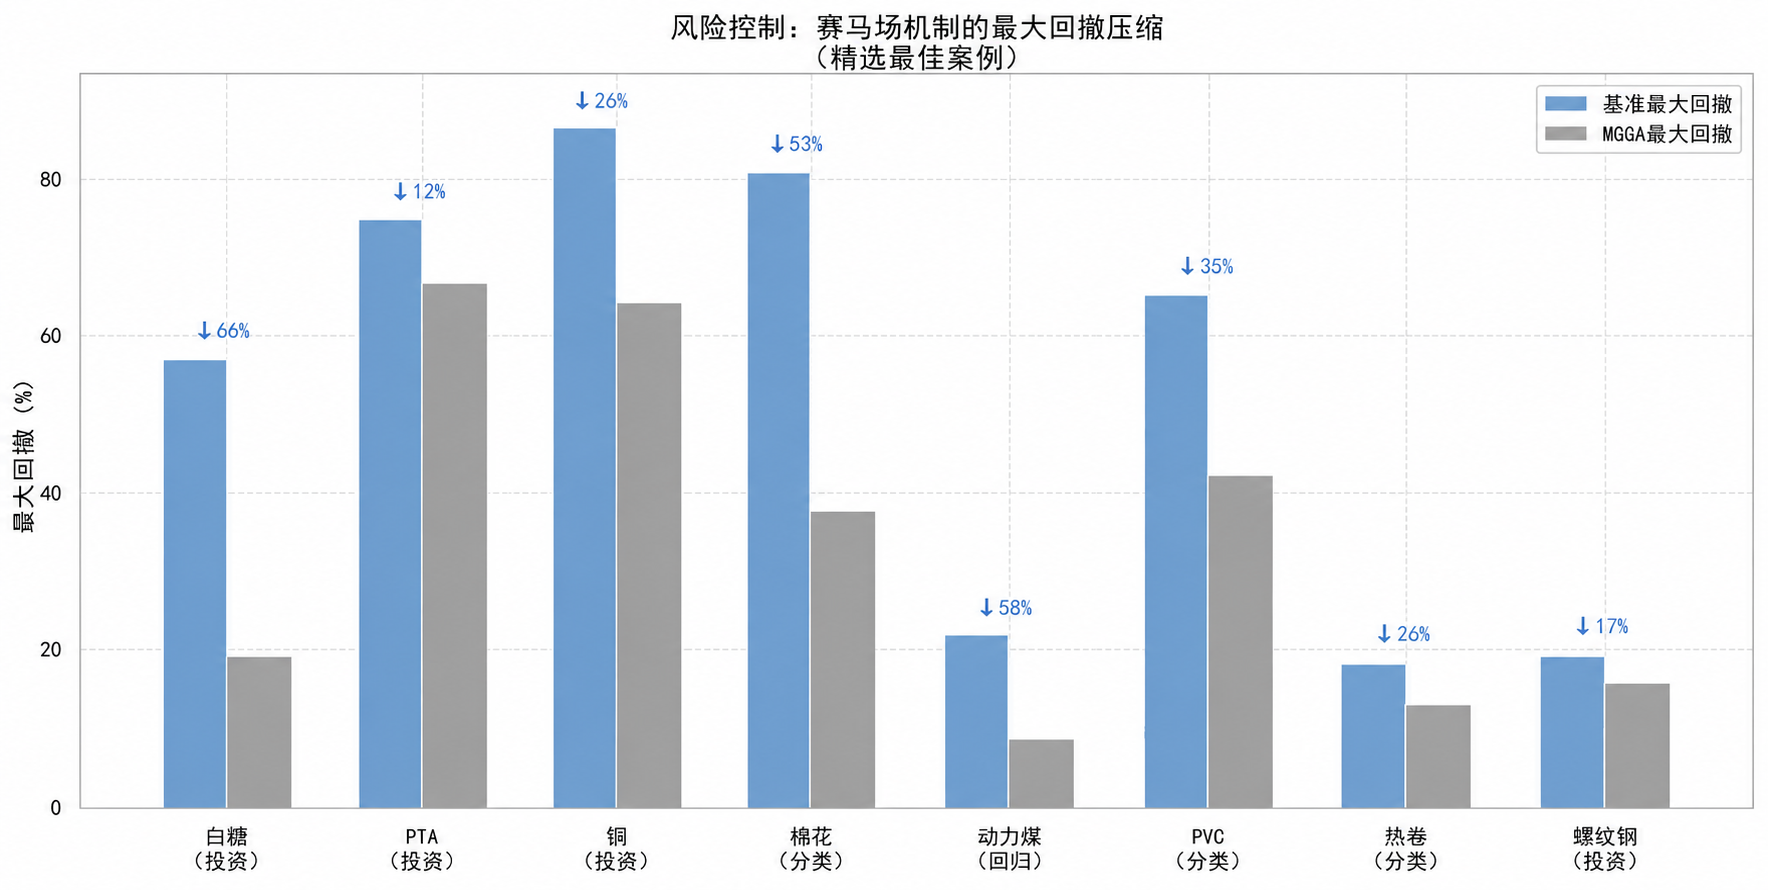
\includegraphics[width=0.8\textwidth]{figures/chap4/图3.24改.png} 
    \caption{赛马场竞争机制的风险控制效果——最大回撤对比（精选最佳案例）}
    \label{fig:highdimcomprehensivebubble}
\end{figure}

棉花分类任务中，基准模型最大回撤为80.94\%，赛马场竞争机制将其压缩至37.97\%（降幅53.1\%）。铜投资任务从86.93\%降至64.65\%（改善25.6\%），PVC分类任务从64.88\%降至42.42\%（改善34.6\%），动力煤回归任务从21.50\%降至8.96\%（改善58.3\%）。上述数据说明，回撤控制方面的改进在多个资产和任务中均有体现。

图\ref{fig:highdimriskreturnmigration}的风险-收益迁移散点图中，每个箭头代表一个资产从基准模型（灰色点）到赛马场竞争机制（红色点）的迁移轨迹，向左上方移动表示回撤降低同时收益提升。
赛马场竞争机制并非简单平均模型输出，而是根据市场环境动态调整模型权重，以兼顾多样性保持与风险控制。

% \begin{figure}[h!]
%     \centering 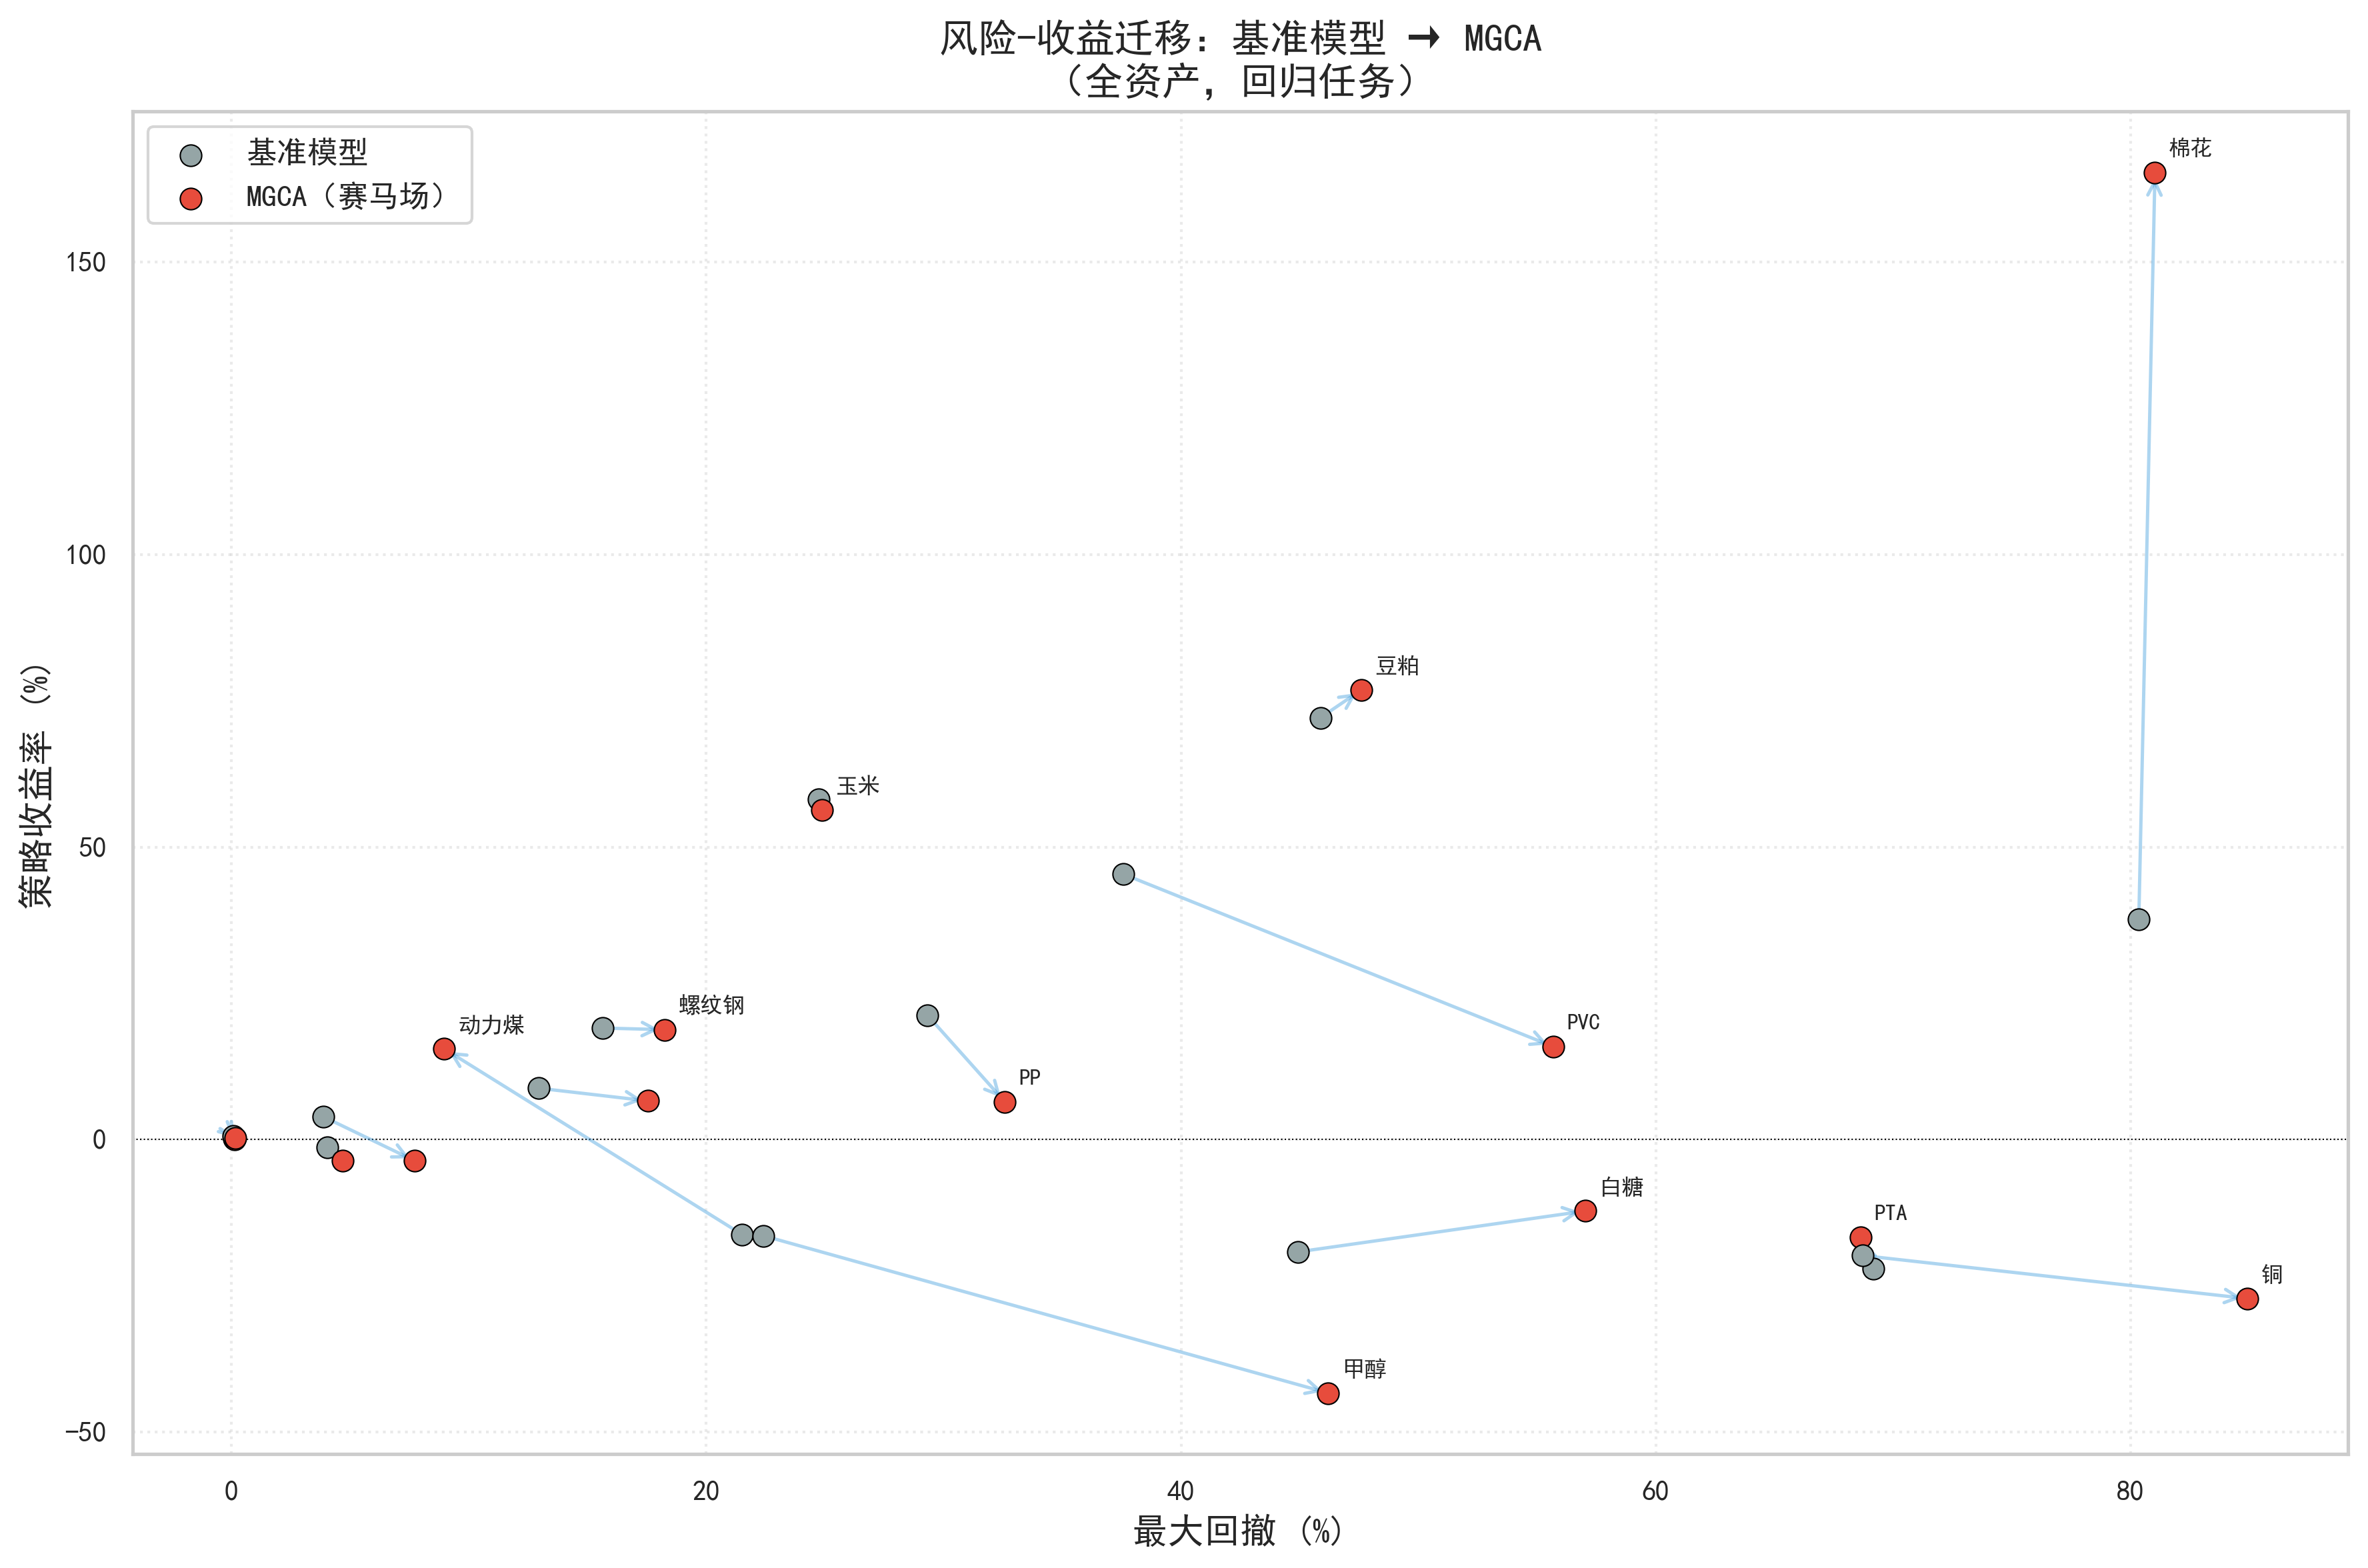
\includegraphics[width=0.8\textwidth]{figures/chap4/fig13_risk_return_migration_cn.png} 
%     \caption{风险-收益迁移散点图（赛马场竞争机制 vs. 基准模型）}
%     \label{fig:highdimriskreturnmigration}
% \end{figure}

\begin{figure}[!htbp]
    \centering 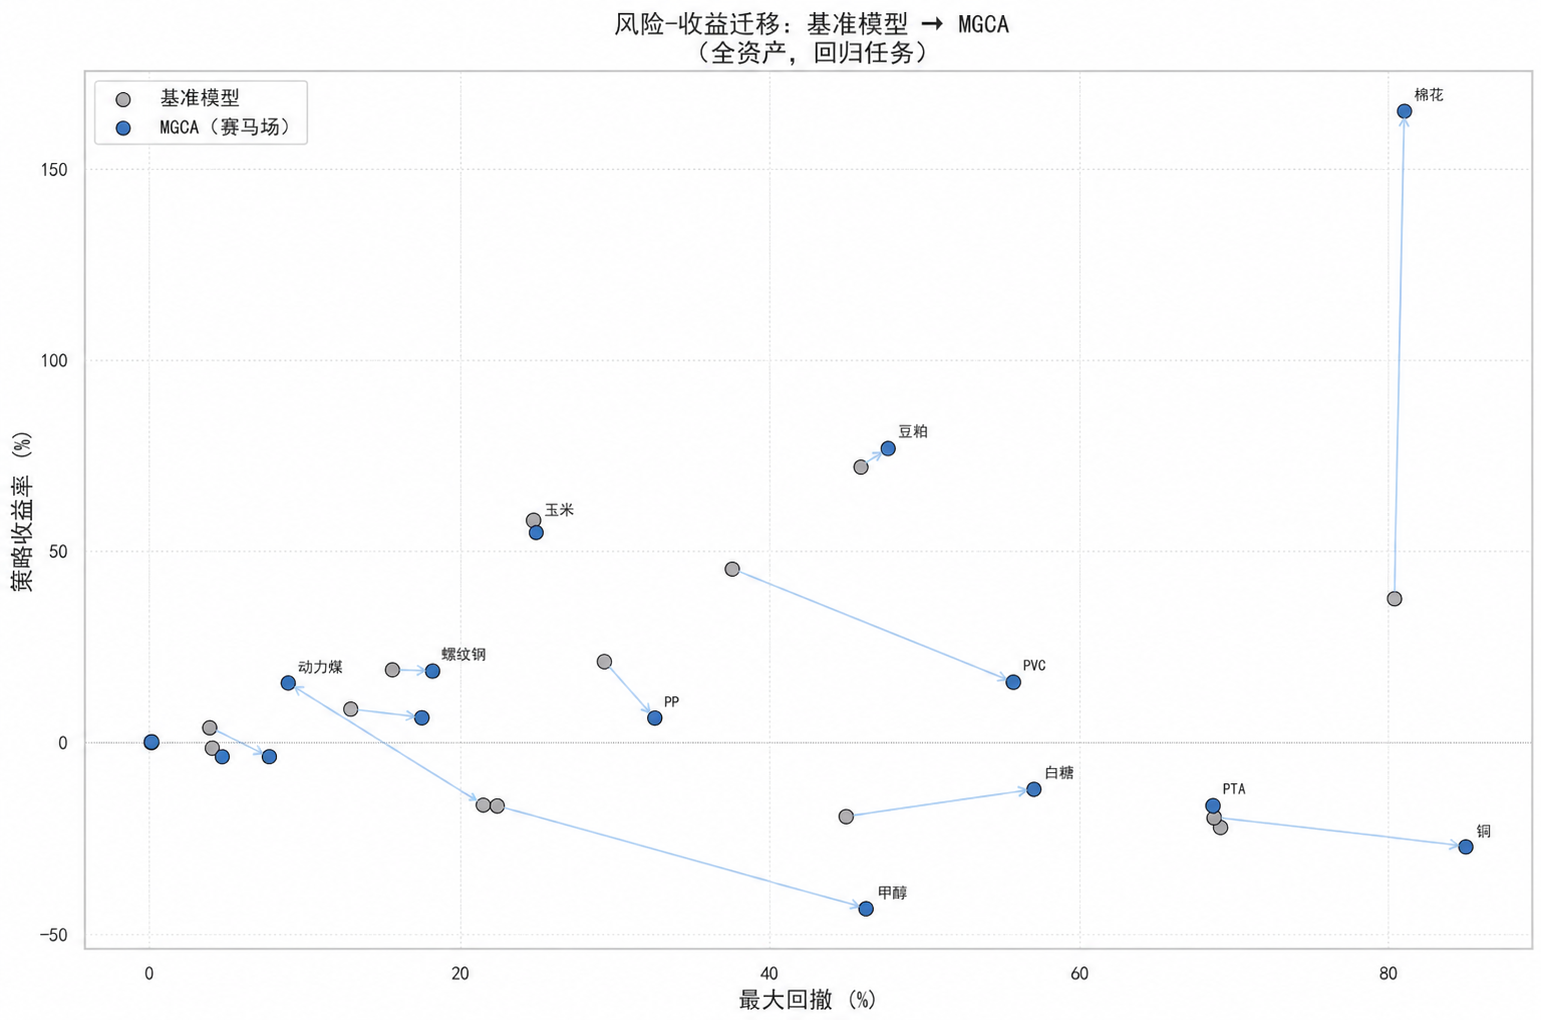
\includegraphics[width=0.8\textwidth]{figures/chap4/图3.25改.png} 
    \caption{风险-收益迁移散点图（赛马场竞争机制 vs. 基准模型）}
    \label{fig:highdimriskreturnmigration}
\end{figure}



\textbf{隐式正则化与过拟合抑制}：传统正则化方法（如一阶/二阶范数惩罚、随机失活）作用于参数空间或特征空间，赛马场竞争机制则在模型选择层面实施筛选——当某个生成器在训练集上表现尚可但验证集性能下降时，动态筛选机制会降低其权重乃至将其淘汰。这种基于泛化性能的动态筛选更直接地面向样本外表现，而不是只通过限制模型复杂度来降低过拟合风险。能源多资产组合和农业多资产组合的亏损转盈利案例（分别实现+202.85\%和+174.13\%的改进）与该解释方向一致：基准模型可能因过度拟合品种间的虚假相关性而亏损，赛马场竞争机制通过持续监控分布外表现，可能降低了对这类相关性的依赖。

\section{本章小结}
本章围绕对冲基金交易决策链条中的高维金融因子建模环节，讨论资产选择背后的因子表征依据形成问题。这里的因子表征依据并不是对交易结果进行事后解释，而是在第2章形成多资产配置入口的基础上，进一步识别哪些高维金融因子能够为资产选择提供稳定、可解释和可迁移的支撑信息。针对高维因子空间中的信息压缩、非对称竞争与过早收敛问题，本章引入了基于赛马场竞争机制的动态演化学习方法。

在方法设计上，本章首先通过多编码器表示学习缓解异构金融特征混合建模带来的结构丢失问题，随后利用赛马场竞争机制组织模型群体进行“评估—培养—淘汰—对齐”的循环演化。成熟—新生模型的双向知识迁移机制，将成熟模型的稳定表征与新生模型的差异化探索结合起来，形成“稳定继承—差异探索—反向校正”的优化过程，从而降低模型群体过快收敛到单一优势路径的风险。由此，本章方法以动态选优回应非对称竞争，以模型替换回应过早收敛，以双向知识迁移回应有效因子表征的持续修正需求。

在实验层面，超过60组对比实验表明，赛马场竞争机制在回撤控制方面的改进较收益率改进更为一致，模型分歧约束在风险暴露控制中的隐性作用也在多个任务类型中有所体现。相关结果说明，该机制并非单纯追求训练误差最小化，而是在模型多样性保持、动态筛选和风险暴露控制之间进行权衡。这种以模型群体交互、动态反馈和策略适应为核心的训练思路，也与多智能体强化学习中通过多主体交互提升复杂环境适应性的研究取向相一致\cite{lowe2017multi}。

本章接续第2章投资组合管理任务，从高维金融因子层面讨论支撑资产选择的表征依据。第2章关注多资产配置结果，本章关注支撑该配置结果的因子表达与动态竞争机制，二者在交易任务链条中形成前后承接。后续第4章将在因子建模基础上转向时序结构识别，讨论因子依据形成之后，如何判断市场结构和交易时机是否成立。
